%%%%%%%%%%%%%%%%%%%%%%%%%%%%%%%%%%%%%%%%%%%%免责声明%%%%%%%%%%%%%%%%%%%%%%%%%%%%%%%%%%%%%%%%%%%%%%%%%%%%
%1. 所有中国科学院大学的单位和个人可任意使用、修改、复制和传播该模板,但需要在作品中标明来源。
%2. 禁止用于任何商业活动。
%3. 限于开发者水平,此模板中可能存在错误,由此造成的任何损失开发者概不负责。
%4. 本模板中包含开发者个人的博士学位论文,使用过程中请严格遵守中国科学院大学相关规定
%5. 本协议未明示授权的其他一切权利仍归开发者所有,用户使用其他权利时必须获得作者的书面同意。
%%%%%%%%%%%%%%%%%%%%%%%%%%%%%%%%%%%%%%%%%%版本号声明%%%%%%%%%%%%%%%%%%%%%%%%%%%%%%%%%%%%%%%%%%%%%%%%%%%%
%   遵照基本软件版本命名规范,该发布版本的主版本号为1,次版本号为3,修订版本号为14,日期版本号为发布日期
%   根据TeX创始人的习惯,任何bug修复版本将按照圆周率在修订版本号后添加一位
%   其他人在读懂代码的基础上重新开发的其他版本可更改主版本号为2,依此类推
%   下一步的思路是放弃CTeX和CJK方案转而使用XeLaTeX引擎和xeCJK包,理论上大部分源代码都可以重用
%   为便于记忆,所有版本均有一个由开发者决定的以某种植物命名的代号,此版本的代号为Clover
%   Version number: 1.3.14_20161208_Release
%        Code name: Clover
%%%%%%%%%%%%%%%%%%%%%%%%注意:凡是用%开头的行都是注释行,TeX不会编译它们%%%%%%%%%%%%%%%%%%%%%%%%%%%%%%%%
%标明文档使用的编码方式。UTF-8是Unicode的一种,使用它可以方便的编辑各种语言。如果没有正确设置编码方式,编译带中文的文档会产生 Package CJK Error: Invalid character code这样的错误。手动设置文档编码方式方法如下:document/document settings/format/UTF-8。使用UTF-8 + XeLaTeX排版中文文档是一种完美选择。但这里我使用的是PDFLaTeX引擎,这样可以一步到位直接生成最后的PDF文件。
% !Mode:: "TeX:UTF-8"
%%%%%%%%%%%%%%%%%%%%%%%%%%%%%%%%%%%%%%%%%%%%%%%%%%%%%%%%%%%%%%%%%%%%%%%%%%%%%%%%%%%%%%%%%%%%%%%%%%%%%%%%
%若打开tex文档报错请使用记事本打开复制里面的内容到新建的tex文档并保存为UTF-8格式即可。这可能是winedt7.0或ctex 套装的bug。注意文件名和保存路径中不要有中文。
%今晚的月色真美。
%另外,不要直接用记事本打开文档进行编辑再保存(虽然你能打开)。因为Windows会在UTF-8 格式的文档前加UNICODE BOM。 而其他软件可能并不这么做。其结果就是Error。
%%%%%%%%%%%%%%%%%%%%%%%%%%%%%%%%%%%%%%%%%%%%%%%%%%%%%%%%%%%%%%%%%%%%%%%%%%%%%%%%%%%%%%%%%%%%%%%%%%%%%%%%
%设置文类为book,其中字号为12 pt,使用A4纸且每章必须从右页开始。该文类默认章节首页使用plain版式,该版式默认页眉空置,页码置于页脚中部。所以后面需要重新定义plain版式。关于文类中各选项的含义请参考http://texblog.org/2013/02/13/latex-documentclass-options-illustrated/#doublesided
\documentclass[12pt, a4paper, twoside, openright]{book}
%调入模板相关说明信息。
%该文件(未发布)仅供开发者个人用于记录和查阅,不含任何代码但有特殊字符,故不要将其调入。
%\input{log}
%调入宏包调用信息。
%input和include命令均能够调入子文档,但include会重启一页
%检测你文档中是否使用已经被淘汰了的宏包以及过时的命令。这个调用应该在最前面甚至文类声明之前。
%\RequirePackage[l2tabu, orthodox]{nag}
%调用xcolor宏包处理颜色,其中可选参数usenames允许使用预定义的颜色(black, blue, brown, cyan, darkgray, gray, green, lightgray, lime, magenta, olive, orange, pink, purple, red, teal, violet, white, yellow)
%可选参数调用colortbl宏包设置彩色表格
\usepackage[usenames,table]{xcolor}
%设置页面布局,这里的参数是word的默认布局
\usepackage [top=2.54cm,bottom=2.54cm,left=3.18cm,right=3.18cm,headheight=15pt]{geometry}
%调用comment宏包添加comment环境
\usepackage{comment}
%调用这两个包用于后面产生文本。它们的顺序很重要,而且不要忘记语言选项,否则是拉丁文http://texblog.org/2011/02/26/generating-dummy-textblindtext-with-latex-for-testing/
\usepackage[english]{babel}
\usepackage{blindtext}
%调用lipsum产生段落。这些段落不是随机生成的,而是从公元前45年的古典拉丁文学著作中截取150个段落中挑选段落。因为这部著作的第一段的前两个词为:Lorem ipsum,因此称为 lipsum。
%http://texblog.org/2011/02/26/generating-dummy-textblindtext-with-latex-for-testing/
\usepackage{lipsum}

%调用ctex宏包处理中文,默认在document环境中插入CJK*环境
%对GB2312格式的文件,引用ctex宏包时无需添加编码格式选项。对于UTF8格式的文件需要加上“UTF8” 参数
\begin{comment}
	ctex宏包的space选项将CJK*环境变为CJK环境。在该环境中排版会保留中文与其他字符之间的空格及换行时自动插入的空格。若发现发现换行时自动插入的空格影响美观请查阅资料进行调整。由于调用中文标题设置宏包会自动加载ctex宏包,故这里将其注释起来。
\end{comment}
%调用titletoc宏包修改目录格式,该宏包调用命令必须在ctexcap之前,否则它将覆盖ctexcap对目录的设置
\usepackage{titletoc}
%\usepackage[space,UTF8]{ctex}
%调用中文标题宏包设置中文标题,该宏包自动加载ctex宏包
\usepackage[UTF8]{ctexcap}
%调用fancyhdr宏包处理页眉和页脚,该宏包默认有0.4 pt的页眉线但无页脚线
\usepackage{fancyhdr}
%调用graphicx宏包来插入图片
\usepackage{graphicx}
%调用hyperrref宏包给各种交叉引用进行超级链接,同时产生PDF中的书签。文档采用UTF-8编码并在参数中选择unicode,否则书签中的中文乱码。该宏包的参数见https://mirrors.tuna.tsinghua.edu.cn/CTAN/macros/latex/contrib/hyperref/doc/options.pdf
\usepackage[colorlinks, unicode, bookmarksnumbered=true, bookmarksopen=true, allcolors=black, allbordercolors=black, hidelinks,pdfpagelabels]{hyperref}
%数学相关宏包
\usepackage{amsmath}
%调用算术宏包calc进行数学运算
\usepackage{calc}
%调用times宏包把\rmdefault设置成Times New Roman字体,把\sfdefault设置成Helvetica,把\ttdefault设置成Courier。 然而它没有更换数学字体。所以这种方法已经不被推荐
%\usepackage{times}
%请尝试用下面的代码替换\usepackage{times}
\usepackage{mathptmx}
\usepackage[scaled=.91]{helvet}
\usepackage{courier}
%This is true Times New Roman, via modern TeX engines(http://tex.stackexchange.com/questions/67768/times-new-roman-font)
%Compile with XeLaTeX or LuaLaTeX
%\usepackage{fontspec}
%\setmainfont{Times New Roman}
%调用数组宏包array插入表格。由于后面的tabularx会加载array,这里将其注释起来。
%\usepackage{array}
%调用tabularx插入可调列宽的表格。该宏包将自动调用array宏包。
\usepackage{tabularx}
%调用ltxtable插入跨页可调列宽的表格。该宏包要求表格代码在独立的tex文档,使用一条命令插入表格。
\usepackage{ltxtable}
%调用multirow插入跨行表格
\usepackage{multirow}
%调用booktabs绘制三线表
\usepackage{booktabs}
%行号宏包,在最终版本中请将其注释起来。单独的宏包调用命令不足以产生行号,在commands.tex中有对应的命令
%\usepackage[switch, pagewise]{lineno}
%调用caption宏包来控制图表标题的格式,但是这里与ccaption宏包冲突故将其注释起来备用
%caption宏包已经是3.x版,所以后面有一个日期来限定其版本,使用前请检查版本
%\usepackage[labelsep=space]{caption}[2004/07/16]
%调用ccaption宏包输入双语标题,不能使用caption2选项(有冲突,原因不明)
%经过试验,ccaption不能使用类似caption的选项。调整标题格式的命令在commands.tex文档中
\usepackage{ccaption}
%调用natbib宏包调整文献条目之间的距离,该宏包还有其他功能
\usepackage[round, authoryear, sort]{natbib}
%调用siunitx输入单位符号
\usepackage[version-1-compatibility]{siunitx}
\usepackage{upgreek}
%调用下划线宏包
%该宏包会将\emph重定义成下划线,如果不希望修改可在调用时增加选项normalem
\usepackage{ulem}
%调用makeidx插入索引
\usepackage{makeidx}
%调用paralist宏包插入列表
\usepackage{paralist}
%调用bbding插入图形符号
\usepackage{bbding}
%ccaption宏包修改图表编号模式需要调用该宏包
\usepackage{remreset}
%调用wasysym宏包在简历中使用性别符号
\usepackage{wasysym}
%调用setspace宏包修改目录的行距
\usepackage{setspace}
%调用footnpag宏包设置脚注以页为排序单位
\usepackage{footnpag}
%调用syntonly宏包使文档编译时只检查语法,这样可以大大缩短长文档的编译时间
%在最终版本中请将该宏包注释起来
%\usepackage{syntonly}
%\syntaxonly
%调用textgreek使用文本模式的希腊字母,然而调用以后系统提示版式设置有问题,运行无法通过
%\usepackage[cbgreek]{textgreek}
%调入修改默认设置的相关命令。
%input和include命令均能够调入子文档,但include会重启一页
\titlecontents{chapter}%
[0em]%
{\vspace{3mm}\heiti}%
{\thecontentslabel}%
{}%
{\titlerule*[0.5pc]{$\cdot$}\bf\contentspage}
\CTEXsetup[beforeskip={0pt},afterskip={15pt},nameformat+={\Large},titleformat+={\Large}]{chapter}
\CTEXsetup[format+={\flushleft\large},beforeskip={3.25ex plus 1ex minus .2ex},afterskip={1.5ex plus .2ex}]{section}
\CTEXsetup[format+={\normalsize},beforeskip={1.5ex plus .2ex minus .2ex}]{subsection}
\CTEXsetup[beforeskip={1.5ex plus .2ex minus .2ex}]{subsubsection}
\setcounter{secnumdepth}{3}
\pagestyle{fancy}
\fancyhf{}
\fancyhead[OC]{\color{darkgray} \nouppercase{ \leftmark}}
\fancyhead[EC]{\color{darkgray} \nouppercase{衣藻鞭毛内运输蛋白IFT46基体定位机制的研究}}
\fancyfoot[OR, EL]{\color{darkgray} \thepage}
\renewcommand{\headrule}{\color{darkgray} \hrule width\headwidth}
\fancypagestyle{plain}{\fancyhf{}%
\fancyhead[OC]{\color{darkgray} \nouppercase{ \leftmark}}%
\fancyhead[EC]{\color{darkgray} \nouppercase{your CHtitle here}}%
\fancyfoot[OR, EL]{\color{darkgray} \thepage}%
\renewcommand{\headrule}{\color{darkgray} \hrule width\headwidth}}
\captiondelim{\space}
\setlength{\abovetopsep}{5pt}
\setlength{\belowrulesep}{0ex}
\setlength{\aboverulesep}{0ex}
\setlength{\belowbottomsep}{0pt}
\addtolength{\bibsep}{-11pt}
\usepackage{microtype}
\newcommand{\tabincell}[2]{\begin{tabular}{@{}#1@{}}#2\end{tabular}}
\makeindex
\captionnamefont{\small}
\captiontitlefont{\small}
\linespread{1.667}


%调入断词声明
%input和include命令均能够调入子文档,但include会重启一页
%断词声明,其中短杠表示潜在的断词位置
\hyphenation{IFT Chlamy-do-monas}
%%%%%%%%%%%%%%%%%%%%%%%%%%%%%%%%%%%%%%%%%%%%%%%%%%%%%%%%%%%%%%%%%%%%%%%%%%%%%%%%%%%%%%%%%%%%%%%%%%%%%%%%
%该命令仅用于调试,将需要调入的文件的文件名加入括号中即可。请在final版本中将其注释掉。
%\includeonly{tableofcotents, references, appendagesA, appendagesB, appendagesC, CV}
%list of all included files
%CHcover, ENcover, announcement, acknowledgement, CHabstract, ENabstract, tableofcotents, chapter1, chapter2, chapter3, %references, appendagesA, appendagesB, appendagesC, CV
%%%%%%%%%%%%%%%%%%%%%%%%%%%%%%%%%%%%%%%%%%%%%%%%%%%%%%%%%%%%%%%%%%%%%%%%%%%%%%%%%%%%%%%%%%%%%%%%%%%%%%%%
%正文环境开始。
\begin{document}
%调入中文封面,不要加拓展名tex。
%input和include命令均能够调入子文档,但include会重启一页
%空行代表重启一个段落。
\begin{titlepage}
\small
\makebox[5em][r]{分类号:}\uline{\makebox[7em][r]{}}\hfill \makebox[5em][r]{密级:}
\uline{\makebox[7em][r]{}}

\makebox[5em][r]{UDC:}\uline{\makebox[7em][r]{}}\hfill \makebox[5em][r]{ 编号:}
\uline{\makebox[7em][r]{}}
\normalsize

\vspace{10mm}

\begin{figure}[!h]
\centering
\graphicspath{{figures/}}
\includegraphics[trim=0 1 1 0, clip=true]{logo.jpg}
\end{figure}

\vspace{10mm}

\begin{center}
\zihao{1} \textbf{博士学位论文}\\[10mm]
\zihao{-3} \textbf{衣藻鞭毛内运输蛋白\ IFT46\ 基体定位机制的研究}\\
\zihao{-3} \textbf{Study on the molecular mechanism of the basal body localization of the intraflagellar transport protein IFT46 in \textit{Chlamydomonas reinhardtii}}\\[10mm]
\end{center}
%在uline命令内部使用粗体命令时水平空白命令如quad会导致加粗失效,这里采用受保护的空格
\large \textbf{姓\qquad 名:}\uline{\hfill\textbf{吕}{} {} \textbf{波}\hfill}\\
\large \textbf{指导教师:}\uline{\hfill\textbf{黄开耀}{} {} \textbf{研究员}{} {} \textbf{博士}\hfill}\\
\large \makebox[5em][]{}\uline{\hfill{\textbf{中国科学院水生生物研究所}}\hfill}\\
\large \textbf{申请学位:}\uline{\hfill{\textbf{理学博士}}\hfill}\\
\large \textbf{学科专业:}\uline{\hfill{\textbf{遗传学}}\hfill}\\
\large \textbf{培养单位:}\uline{\hfill{\textbf{中国科学院水生生物研究所}}\hfill}\\
\large \textbf{授予单位:}\uline{\hfill{\textbf{中国科学院大学}}\hfill}\\[4mm]
\begin{center}
\textbf{二零一七年五月}
\end{center}
\end{titlepage}

\vspace*{10mm}
\thispagestyle{empty}

%调入英文封面,不要加拓展名tex。
%input和include命令均能够调入子文档,但include会重启一页
\begin{titlepage}
\vspace*{20mm}
\centering
\large
\textbf{
The Title of Your Thesis\\[40mm]
By\\
Bo\quad Lv\\[30mm]
A Dissertation Submitted to\\
The University of Chinese Academy of Sciences\\
In partial fulfillment of the requirement\\
For the degree of\\
Doctor of Science\\
\vspace{20mm}
Institute of Hydrobiology, Chinese Academy of Sciences\\
May, 2017
}
\end{titlepage}

\vspace*{10mm}
\thispagestyle{empty}





%调入声明,不要加拓展名tex。
%input和include命令均能够调入子文档,但include会重启一页
%空行代表重启一个段落。
\chapter*{作者声明}
\thispagestyle{empty}
\vspace{2em}
本人郑重声明:所呈交的学位论文,是本人在导师的指导下,独立进行研究工作所取得的成果。除文中已经注明引用的内容外,本论文不包含任何其他个人或集体已经发表或撰写过的作品成果。对本文的研究作出重要贡献的个人和集体,均已在文中以明确方式标明。

本人完全意识到本声明的法律结果由本人承担。
\vspace{2em}
%\large
\zihao{4}

\hfill 指导老师:\uline{\makebox[6em][l]{}}(签名)
\vspace{1em}

\hfill 论文作者:\uline{\makebox[6em][l]{}}(签名)
\vspace{1em}

\hfill 年\qquad 月\qquad 日
\normalsize

\newpage
\thispagestyle{empty}
%%%%%%%%%%%%%%%%%%%%%%%%%%%%%%%%%%%%%%%%%%%%%%%%%%%%%%%%%%%%%%%%%%%%%%%%%%%%%%%%%%%%%%%%%%%%%%%%%%%%%%%%
%开始前文区。
\frontmatter
%设置前文区的页码为大写罗马数字,默认为小写罗马数字。
\pagenumbering{Roman}
%调入致谢,不要加拓展名tex
%input和include命令均能够调入子文档,但include会重启一页
\chapter{致\quad 谢}
\renewcommand{\leftmark}{致\quad 谢}

\blindtext

\blindtext

\blindtext

\blindtext

\vspace{3em}

\hspace{25em}吕\quad 波
\vspace{1em}

\hfill 二零一七年五月于武汉东湖之滨


%调入中文摘要,不要加拓展名tex。
%input和include命令均能够调入子文档,但include会重启一页
\chapter{中文摘要}
\renewcommand{\leftmark}{中文摘要}

\blindtext
%调入英文摘要,不要加拓展名tex。
%input和include命令均能够调入子文档,但include会重启一页
%空行代表重启一个段落。
\chapter{Abstract}
%直接在奇数页页眉中显示章标题会多处一些章标题内部编号,这里重新定义\leftmark,后续所有章节都要重新定义
\renewcommand{\leftmark}{Abstract}
Eukaryotic cells evolved different types of organelles that carry out specialized functions. One of them is the cilium, also known as flagellum (interchangeable terms), which is found on most eukaryotic cells. Cilia are hairlike microtubule-based organelles that protrude from the cell surface and are composed of ciliary membrane, ciliary matrix and axoneme templated by a basal body. Cilia primarily play two vital roles. One is to function as a cellular motor to move either the cell itself or surrounding liquids/particles. The other function of cilia is to serve as a hub for cellular signaling. Defects in ciliary structures and functions in humans lead to diseases commonly referred to as `ciliopathies', such as blindness, deafness, hyperdactylism, heterotaxy and polycystic kidney disease.

The formation and maintenance of cilia, as well as ciliary signaling, depend on intraflagellar transport (IFT), a bidirectional movement of granular particles between the outer doublet microtubules and the flagellar membrane along the axoneme. More than 22 IFT proteins form at least three biochemically distinct complexes, namely IFT-A, IFT-B1 and IFT-B2. In addition to the dynamic movement of IFT in cilia, nearly all subunits of IFT complex, cargos and motor proteins are concentrated at the basal body where they upload, download or couple. However, the mechanism of the basal body localization of IFT subunits, which is one of the key steps in the initiation of ciliogenesis, remains largely unknown.

In this study, we explored the molecular mechanism of the basal body localization of IFT46. Firstly, we fused Citrine Yellow fluorescent protein (YFP) to the C-terminus of IFT46. When expressed in \textit{ift46-1}, rescued strains have full-length flagella and swim normally. The average ciliary lengths and the percentages of ciliated cells of the rescued strains are akin to those of wild-type (WT) cells. The anterograde and retrograde transport velocities and frequencies of IFT46::YFP are similar to results published previously. In summary, these data demonstrate that the 28 kDa YFP tag does not affect the function of IFT46. The confocal imaging results showed that the negative control, YFP, accumulates around the nuclei in \textit{ift46-1 YFP}. IFT46::YFP accumulates at basal bodies and localizes in a dotted pattern along the flagella, just as other IFT subunits do. Moreover, the punctate pattern of IFT46::YFP along the flagella is more obvious when examined by total internal reflection fluorescence microscopy.  To identify the targeting sequence in IFT46 responsible for its basal body localization, we generated and expressed a series of truncated IFT46 constructs fused with YFP in \textit{ift46-1}. We found that IFT46-C1 may contain the basal body targeting sequence of IFT46. Further research showed that the C-terminus without the glycine-rich tail (246-321 aa, BBTS3) could also target YFPs to the basal body. Moreover, we found that BBTS3 can also target IFT46 to cilia. IFT46-C1 and BBTS3 are able to move along the axoneme, and are
likely to be incorporated into IFT-B complexes as part of IFT46. These results demonstrate that the basal body and ciliary targeting of IFT46 require BBTS3.

We next determined whether the basal body localization of IFT46 depends on other IFT components. Accordingly, we expressed full-length IFT46::YFP and IFT46-C1::YFP in \textit{bld1}, \textit{ift88}, \textit{fla10-2} and \textit{dhc1b}. Positive transformants expressing IFT46::YFP or IFT46-C1::YFP were screened using western blotting with an antibody against GFP. We also examined the subcellular localization of IFT46 in \textit{ift81-2} and \textit{ift122-1} strains using immunostaining. The basal body localization of IFT46 is independent of IFT122, IFT88, IFT81, FLA10 or DHC1b. Surprisingly, the basal body localization of IFT46 depends upon IFT52, but not vice versa. IFT46::YFP and IFT46-C1::YFP were targeted to the basal body region in \textit{bld1 IFT46::YFP IFT52::3HA} and \textit{bld1 IFT46-C1::YFP IFT52::3HA}. These results further demonstrate that the basal body localization of IFT46 relies on IFT52. IFT46-C1 interacts with IFT52 through its C1 domain, which is mediated by the L285 and L286. That means IFT52 binds to and recruits IFT46 to the basal body region. Finally, we find that NLS-tagged IFT52C can recruit IFT46 to nuclei. Based on previous studies and our results here, we conclude that IFT52 and IFT46 are preassembled in the cytoplasm and are delivered to the basal body through vesicular transport or nonvesicle-mediated ways.

Our study here paves the way for the comprehensive deciphering of the mysteries of the basal body localizaiton of IFT proteins. We also shed new light on the atlas of interactions between the IFT proteins, motors and cargos at the basal body. These progresses are of vital importance to resolve the mechanism of ciliary assembly and disassembly. Furthermore, to some extent, our study can guide the prevention and treatment of ciliopathies through the regulation of ciliogenesis and ciliary functions.

\vspace{10mm}

\noindent \textbf{Key Words:\ }\textit{Chlamydomonas}, Intraflagellar transport, Basal body, Targeting sequence

%调入目录,不要加拓展名tex。
%input和include命令均能够调入子文档,但include会重启一页
\renewcommand{\contentsname}{目\quad 录}
\renewcommand{\bibname}{参考文献}
\renewcommand{\indexname}{索引}
\cleardoublepage
\phantomsection
\addcontentsline{toc}{chapter}{目\quad 录}
\setcounter{tocdepth}{3}
\renewcommand{\leftmark}{目\quad 录}
\begin{spacing}{1.0}

\tableofcontents

\end{spacing}

%%%%%%%%%%%%%%%%%%%%%%%%%%%%%%%%%%%%%%%%%%%%%%%%%%%%%%%%%%%%%%%%%%%%%%%%%%%%%%%%%%%%%%%%%%%%%%%%%%%%%%%%
%开始主文区。
\mainmatter
%设置主文区的页码为阿拉伯数字。
\pagenumbering{arabic}
%调入第一章,不要加拓展名tex。
%input和include命令均能够调入子文档,但include会重启一页
%空行代表重启一个段落。
\chapter{引\quad 言}
%直接在奇数页页眉中显示章标题会多处一些章标题内部编号,这里重新定义\leftmark,后续所有章节都要重新定义
\renewcommand{\leftmark}{第一章\quad 引\quad 言}
真核细胞利用不同的细胞器执行特定功能,其中之一是纤毛/鞭毛。纤毛是广泛存在于真核细胞表面的毛发状结构,它由基体、轴丝、基质和纤毛膜组成\ \citep{Mizuno2012,Satir2007}。纤毛的功能可分为两大类\ \citep{Satir2007},其一是作为细胞的马达驱动细胞自身或周围的流体/颗粒物运动。另一类是参与细胞对胞内外环境的感知\ \citep{Ishikawa2011,Mourao2016,Singla2006,Wood2015}。 人体纤毛结构或功能的缺陷可导致诸如多囊肾、眼盲、内脏异位及骨骼异常等纤毛病\ \citep{Fliegauf2007,Gerdes2009,Hildebrandt2011,Hildebrandt2007}。

纤毛的形成、维持及信号传导依赖鞭毛内运输(intraflagellar transport, IFT)\citep{Ishikawa2011,Mourao2016,Pedersen2008,Scholey2003}。IFT\ 是轴丝和纤毛膜之间的颗粒物沿纤毛作双向运动\ \citep{Kozminski1993}。正向\ IFT(从基部到顶部)由\ kinesin-2\ 驱动\ \citep{Kozminski1995,Miller2005,Ou2005,Pan2006,Snow2004,Walther1994},反向\ IFT(从顶部到基部)则由胞质动力蛋白\ 2/1b\ 介导\ \citep{Hou2004,Pazour1999}。目前已经鉴定到的\ IFT\ 蛋白有\ 22\ 个,这些蛋白形成了三个独特的复合物,它们分别是\ IFT-A、IFT-B1\ 和\ IFT-B2\ \citep{Taschner2016,Taschner2016a}。\ IFT\ 可以与它携载的货物一起形成周期性的\ IFT\ 火
车\ \citep{Pigino2009,Stepanek2016,Vannuccini2016,Lechtreck2015,Lechtreck2017}。正向\ IFT\ 火车长约\ \SI{233}{\nm},沿二联管中的\ B\ 管运动。反向\ IFT\ 火车长约\
\SI{209}{\nm},沿二联管中的\ A\ 管运动\citep{Pigino2009,Stepanek2016,Vannuccini2016}。此外,IFT\ 蛋白还参与其他生物学过程如囊泡分泌、细胞分裂、免疫突触及微管纳米管的形成等\
\citep{Baldari2010,Borovina2013,Griffiths2010,Inaba2015,Wood2012,Fu2016}。

纤毛内部无蛋白合成系统,大部分纤毛结构蛋白和信号分子必须在细胞体中合成然后通过\ IFT\ 运输到纤毛内部。因此,几乎所有的\ IFT\ 蛋白和马达分子都富集在基体周围。IFT-B\ 蛋白和正向分子马达在基体呈半环三裂弧状,IFT-A\ 蛋白和反向分子马达则呈半环双裂弧分布\ \citep{Brown2015,Deane2001}。而且,IFT-B\ 和\ IFT-A\ 蛋白之间存在部分共定位\ \citep{Brown2015}。然而,作为纤毛形成起始阶段的关键步骤,IFT\ 蛋白基体定位的分子机制尚不明确。由于\ IFT\ 蛋白如\ IFT46\ 在纤毛再生过程中定位在来源于反式高尔基体网络的囊泡上,Woods\ 等人认为\ IFT\ 可能先加载在囊泡上并招募货物然后靶向运输到基体\
\citep{Wood2014}。然而这一观点有待进一步证实。许多纤毛蛋白(尤其是纤毛膜蛋白)含有纤毛定位序列(ciliary targeting sequences, CTSs)\citep{Bhogaraju2013,Malicki2014}。这些\ CTSs\ 介导了目标蛋白的基体和纤毛定位。然而,CTSs\ 种类繁多,如\ G\ 蛋白偶联受体第三个胞内环上的基序、Ax(S/A)xQ\ 基序、RVxP\ 基序、核定位信号(nuclear localization signal, NLS)以及\ SUMOylation。这表明多种不同的运输系统参与了这一过程\ \citep{Bhogaraju2013,Malicki2014,Dishinger2010,McIntyre2015}。尽管如此,IFT\ 蛋白中不存在已知的\ CTSs。

已知某些蛋白如\ BBS7、BBS8、C2cd3、CCDC41、OFD1、Rsg1\ 和\ TTBK2\ 影响特定\ IFT\ 蛋白的基体定位\ \citep{Blacque2004,Brooks2013,Goetz2012,Joo2013,Ye2014}。然而它们的功能不具有特异性\ \citep{Toriyama2016}。2016\ 年,研究人员发现包括\ Jbts17、Intu、Fuz、Wdpcp\ 和\ Rsg1\ 在内的纤毛形成与平面极性效应蛋白(ciliogenesis and planar polarity effectors, CPLANE)可将\ IFT-A\ 的外周亚基招募到基体\ \citep{Brooks2012,Toriyama2016}。尽管\ CPLANE\ 蛋白可能只是影响\ IFT-A\ 外周亚基的组装或稳定性,这仍然是该领域的重大突破之一\ \citep{Toriyama2016}。

本研究中我们关注的是\ IFT46\ 基体定位的分子机制。我们拟通过表达截短片段的方式鉴定\ IFT46\ 的基体和纤毛定位序列,同时我们将通过一系列细胞、生化和遗传学研究与定位序列相互作用的蛋白。最终我们将初步探明\ IFT46\ 基体定位的分子机制。这一研究有助于最终阐明\ IFT\ 蛋白基体定位以及与货物相互作用的机制,同时对调控纤毛形成及纤毛功能也具有重要的指导意义。




%调入第二章,不要加拓展名tex。
%input和include命令均能够调入子文档,但include会重启一页
%空行代表重启一个段落。
\chapter{文献综述}
%直接在奇数页页眉中显示章标题会多处一些章标题内部编号,这里重新定义\leftmark,后续所有章节都要重新定义
\renewcommand{\leftmark}{第二章\quad 文献综述}
\renewcommand{\figurename}{图}

鞭毛/纤毛是一类突出在细胞表面的毛发状细胞器,广泛存在于真核细胞\
\citep{Ishikawa2011,Hildebrandt2011,Scholey2003,Fliegauf2007}。鞭毛可执行运动、感受和信号传导等功能,其结构或功能异常将导致眼盲、耳聋、多囊肾、多囊肝、肥胖和癌症等纤毛病\
\citep{Fliegauf2007,Hildebrandt2007,Hildebrandt2011,Gerdes2009}。纤毛的形成与解聚依赖鞭毛内运输复合物\
\citep{Bhogaraju2013,Dentler2005,Engel2012,Morga2013,Pedersen2008,Scholey2003,Taschner2016,Mourao2016},该复合物含有至少\ 22\ 个亚基\ \citep{Taschner2016a,Taschner2016,Katoh2016}。鞭毛内运输复合物相关基因的突变将导致细胞没有或仅有极短的鞭毛,研究这些蛋白的结构和功能显得极为重要。在鞭毛形成与解聚过程中,IFT\ 蛋白会富集在基体周围\ \citep{Toriyama2016,Brown2015}。然而其具体的分子机制尚不清楚。除酵母和高等植物外,几乎所有的模式生物都可用于鞭毛生物学的研究。然而,莱茵
衣藻\ (\textit{Chlamydomonas reinhardtii}, 以下简称衣藻)\ 具有某些独特的优势。衣藻具有一对等长的鞭毛,是研究鞭毛相关问题的模式生物之一\
\citep{Goodenough1992,Harris2001}。 本章将对衣藻、鞭毛的结构和功能、鞭毛内运输及蛋白纤毛定位机制等研究的进展进行综述。

\section{衣藻简介}
\subsection{衣藻的基本特征}
衣藻广泛分布在世界各地的泥土和淡水水体中\ \citep{Mussgnug2015},它是一种单细胞真核绿藻,直径约\
\SI{10}{\um},素有“绿色酵母”之称\ \citep{Goodenough1992,Rochaix1995,Flowers2015}。整个衣藻细胞被富含羟脯氨酸的糖蛋白组成的细胞壁围绕\ \citep{Mussgnug2015}。细胞内部含一个大的杯状叶绿体,约占细胞总体积的\ 40\% (图\ \ref{fig:2.1})。 在叶绿体中有一个主要由蛋白组成的淀粉核/蛋白核,其四周被淀粉颗粒环绕(图\ref{fig:2.1})。杯状叶绿体的凹陷处是衣藻的细胞核(图\ \ref{fig:2.1})。此外,衣藻细胞还有两根长度约\ 10-\SI{12}{\um}\ 直径约\ \SI{200}{\nm}\ 的鞭毛和一个用于感光的眼
点\ \citep{Lechtreck2013} (图\ \ref{fig:2.1})。衣藻叶绿体基因组富含\ AT,但衣藻核基因组富含\ GC,其平均\ GC 含量为\ 64\%,基因编码区的\ GC\ 含量高达\ 68\%\ \citep{Blaby2014,Grossman2007}。

%开始图片浮动体环境,其中!表示取消严谨限制,h表示在此处插入,t表示在本页或下一页顶部插入
\begin{figure}[!htbp]
%居中对齐
\centering
%设置图片搜索路径,每个路径用{}括起来
\graphicspath{{figures/}}
%插入图片并设置图片宽度为文本宽度减10mm
\includegraphics[width=\textwidth-80mm]{fig2-1.jpg}
%生成中英双语标题
{\setstretch{1.667}
\bicaption[fig:2.1]{图}{衣藻细胞结构示意图\ \citep{Avasthi2014}。图中标记的是已经鉴定的常见细胞器。}{Figure}{Diagram of the cell structure of a \textit{Chlamydomonas\/} cell \citep{Avasthi2014}. Prominent organelles identified are marked.}
\par}
%结束图片浮动体环境
\end{figure}

\subsection{衣藻作为模式生物的优势}
作为研究光合作用、油脂代谢、趋光性\ \citep{Kianianmomeni2014}、鞭毛的形成与解聚、鞭毛运动、蛋白质合成、细胞壁合成、配子形成、细胞周期调控和交配等过程的模式生
物\ \citep{Mussgnug2015,Gallaher2015,Flowers2015},衣藻具有以下特征和优势:

\begin{asparaitem}[\DiamondSolid]
\item 生长迅速,倍增时间仅\ 8-12\ 小时\citep{Blaby2014}。

\item 培养简便,成本低\ \citep{Sager1953,Harris1989,Flowers2015}。 此外,衣藻的细胞周期可以简单的通过调节光暗比进行同步\ \citep{Blaby2014,Hlavova2016}。

\item 在光照条件下,衣藻可进行光能自养。在黑暗条件下,衣藻可在含醋酸根离子的培养基中通过化能异养生存\ \citep{Blaby2014,Flowers2015}。这种灵活的代谢特性使得研究人员可以筛选出无法进行光合作用的突变体进而对光合作用相关基因进行研究\ \citep{Jinkerson2015}。

\item 衣藻鞭毛与哺乳动物细胞上的鞭毛高度同源,这使得衣藻可以作为研究纤毛相关疾病的模式系统。而且衣藻鞭毛是非必须的,这使得研究人员可以筛选出鞭毛结构和功能缺陷的突变体从而开展相关
    研究\ \citep{Blaby2014}。

\item 因衣藻既可进行有性繁殖,又可进行无性繁殖,所以可对其进行经典遗传学
    分析\ \citep{Kates1964,Flowers2015} (图\ \ref{fig:2.2})。 衣藻的营养细胞是单倍体。在缺氮条件下,营养细胞可以形成单倍体配子\ \citep{Gallaher2015}。 两种不同交配型的配子(mt+\ 和\ mt-)可以结合形成二倍体合子(图\ \ref{fig:2.2})。合子细胞没有鞭毛,它是这种生物在泥土中的休眠形式。在光照条件下,合子细胞可进行减数分裂产生四个有鞭毛的营养细胞。但是在生长条件良好的情况下,减数分裂产生的四个子细胞在从母细胞壁中释放之前会进行二到三轮有丝分裂。这样母细胞壁中就可能出现四、八或十六,甚至更多子细胞\ \citep{Jinkerson2015}。

\item 衣藻在营养生长阶段为单倍体,便于筛选突变体\ \citep{Avasthi2013,Li2016}。 突变后可立刻观察到表型而不需要进行杂交\ \citep{Jinkerson2015,Mussgnug2015}。

\item 针对衣藻的转化技术已经非常成熟。利用基因枪、玻璃珠转化或者电转化可以将外源\ DNA\ 导入到核基因组中\
    \citep{Jinkerson2015,Mussgnug2015,Kang2015,Neupert2009,Yamano2013}。 虽然是随机插入,但是插入位点的侧翼序列可以通过巢式\ PCR\ 和二代测序进行鉴定\
    \citep{Gonzalez-Ballester2011,Primers2007,Zhang2014,Li2016,Cheng2017}。尽管效率较低,外源\ DNA\ 也可通过同源重组定向插入到叶绿体和线粒体基因组中\ \citep{Kindle1990,Shimogawara1998}。 此外,衣藻中可用的筛选标记也非常丰富,如巴龙霉素抗性基因、潮霉素抗性基因、壮观霉素抗性基因、锌霉素抗性基因、卡那霉素抗性基因和四环素抗性基
    因等\ \citep{Mussgnug2015,Garcia-Echauri2015,Cerutti1997,Barahimipour2016}。 报告基因如氧气依赖的荧光蛋白\
\citep{Shaner2013,Harris2016,Ormo1996,Fuhrmann1999,Franklin2002,Hakkila2003,Heim1995,Phillips2001,Prasher1992,Onishi2016,Rasala2014,Lauersen2015}
    、黄素依赖的荧光蛋白\ \citep{Mukherjee2015}、 荧光素酶\
    \citep{Minko1999,Shao2008,Fuhrmann2004,Lauersen2013}、木聚糖酶\ \citep{Rasala2012}、 芳基硫酸酯酶\ ARS2\ \citep{Specht2014} 及各种细胞器靶向标记物也已被广泛使
    用\ \citep{Minko1999,Lauersen2015,Rasala2014}。

%开始图片浮动体环境,其中!表示取消严谨限制,h表示在此处插入,t表示在本页或下一页顶部插入
\begin{figure}[tbhp]
%居中对齐
\centering
%设置图片搜索路径,每个路径用{}括起来
\graphicspath{{figures/}}
%插入图片并设置图片宽度为文本宽度减10mm
\includegraphics[width=\textwidth-10mm]{fig2-2.jpg}
%生成中英双语标题
{\setstretch{1.667}
\bicaption[fig:2.2]{图}{衣藻生活史示意图\ \citep{Zhao2001}。图中加号(+)代表正配子,减号(-)代表负配子。}{Figure}{Diagram of the \textit{Chlamydomonas reinhardtii}'s life cycle \citep{Zhao2001}. Plus sign and minus sign represent mating type plus and minus respectively.}
\par}
%结束图片浮动体环境
\end{figure}

\item RNA干扰已被广泛用于衣藻核基因的敲降\
    \citep{Hu2014,Schmollinger2010,Zhao2009,Molnar2009}。Cre/loxP\ 系统也已开始在衣藻中
    应用\ \citep{Kasai2016}。 尽管效率有待提高,锌指核酶和\ TALEs\ 已被用于衣藻核基因的编辑\
    \citep{Jinkerson2015,Mussgnug2015}。 近年来被广泛应用的基因魔剪\ CRISPR/Cas9\
    也已被用于衣藻研究,但这种方法在衣藻中的应用需要进一步开发\
    \citep{Jiang2014,Shin2016,Baek2016,Lander2016a}。

\item 关于衣藻的遗传信息非常丰富
\footnote{\textit{Chlamydomonas} Resource Center, www.chlamycollection.org},其核基因组、线粒体基因组和叶绿体基因组均以被测定\
    \citep{Grossman2003,Maul2002,Mussgnug2015,Gallaher2015,Flowers2015}。衣藻核基因组含十七条染色体\
    \citep{Dutcher1991},约\ 111.1\ Mbp,含\ 17741\ 个基因,叶绿体基因组约\ 203 kbp,含\ 99\ 个基因,线粒体基因组约\ 16 kbp,含\ 8\ 个基因\ \citep{Jinkerson2015,Mussgnug2015}。此外还有大量的\ EST\ 信息可供查询
    \footnote{\textit{Chlamydomonas reinhardtii} EST index, http://est.kazusa.or.jp/en/plant/chlamy/EST/}。 有可供使用的柯斯质粒和酵母人工染色体文库及\ BAC\ 文库\
    \citep{Blaby2014}。

\item 衣藻存在碳浓缩机制,对相关基因的研究和利用有望增强\ C3\ 植物的光合作用效率\
    \citep{Wang2011,Wang2014b,Atkinson2015,Grossman2007}。 此外,衣藻在缺氮条件下可以积累达细胞干重\ 20-30\%\ 的三酰甘油,可用于制备生物柴油\ \citep{Ho2014}。衣藻在缺硫条件下可积累氢气,是生产这种清洁能源的理想生物反应器\ \citep{Ho2014}。

\end{asparaitem}

鉴于这些优势,利用衣藻作为模式生物进行的研究逐年增多。除了传统的基础研究,衣藻在生物能源、生物医药等新技术领域的研究和应用也逐渐成为热点\
\citep{Franklin2004,Fuhrmann2004,Leon-Banares2004,Mayfield2007,Gallaher2015,Kempinski2015,Wijffels2010,Lauersen2013} 。在分子农业领域,经过遗传改造的衣藻已被用于生产哺乳动物血清淀粉蛋白、人抗体蛋白、人血管内皮生长因子、人乳头瘤病毒疫苗、HIV\ 抗原\ P24\ 等生物制剂\ \citep{Barahimipour2016}。 同时,衣藻在产氢和产油等方面的研究也正在如火如荼的开
展\ \citep{Gallaher2015,Flowers2015,Kempinski2015,Greenly2015}。

%开始图片浮动体环境,其中!表示取消严谨限制,h表示在此处插入,t表示在本页或下一页顶部插入
\begin{figure}[htb!]
%居中对齐
\centering
%设置图片搜索路径,每个路径用{}括起来
\graphicspath{{figures/}}
%插入图片并设置图片宽度为文本宽度减10mm
\includegraphics[width=\textwidth]{fig2-5.jpg}
%生成中英双语标题
{\setstretch{1.667}
\bicaption[fig:2.5]{图}{人体各种类型的细胞表面均有纤毛分布\ \citep{Fliegauf2007}。}{Figure}{Cilia extend from the surface of almost all cell types of the human body \citep{Fliegauf2007}.}
\par}
%结束图片浮动体环境
\end{figure}

\section{鞭毛简介}
\subsection{鞭毛的结构}
鞭毛从十九世纪末期被发现至今已有一百多年的历史,它们是一类保守的细胞器(图\ \ref{fig:2.5})。除酵母和高等植物外,鞭毛存在于几乎所有真核细胞
表面\ \citep{Czarnecki2012,Wheatley1996,Brooks2014,Fliegauf2007}。 鞭毛的形态和结构具有多样性,但总体上可被分为运动纤毛(出现在少数类型细胞上,一般为多生)和初级纤毛(出现在多种类型细胞上,一般为单生)两大类\ \citep{Gluenz2010,Gibbons1960}(图\ \ref{fig:2.5})。运动纤毛为\ 9+2\ 结构,初级纤毛为\ 9+0\ 结构。需要注意的是节点纤毛\footnote{nodal cilia}虽然为\ 9+0\ 结构,但可以借助\ A\ 管上的动力臂进行
运动\ \citep{Czarnecki2012} (图\ \ref{fig:2.5})。 在这两类纤毛中,运动纤毛一般出现在多纤毛细胞上且在进化上可能早于初级纤毛\ \citep{Warner2013}。鞭毛结构的这种保守性使得其直径维持在\ 160-280 nm \ 之间\
\citep{Huang2016}。其中纤毛基部偏粗,远端偏细\ \citep{Huang2016}。 这一方面是因为基部存在突起(可能是将要分泌到环境中的囊泡),另一方面是因为微管二联管在远端变成单管\
\citep{Huang2016,Wang2014,Wood2013}。

基于鞭毛结构的保守性,这里我们主要介绍衣藻鞭毛的结构。正常的衣藻细胞有两根运动鞭毛,靠近眼点的称为顺式鞭毛\footnote{cis flagellum},远离眼点的称为反式鞭毛\footnote{trans flagellum}。衣藻鞭毛主要由轴丝、过渡区、鞭毛颈(纤毛膜外部的蛋白鞘)和鞭毛膜
以基体为模板形成\ \citep{Hilbert2016,Kitagawa2011}。基体为特化的中心粒(图\ \ref{fig:2.6})。轴丝为\ 9+2\ 结构,外部九个二联管的\ A\ 管上伸出外部动力臂
\footnote{ODA, outer dynein arm}、内部动力臂\footnote{IDA, inner dynein arm}和放射辐条等结构
(图\ \ref{fig:2.6})。相邻二联管的\ A\ 管和\ B\ 管之间由连接蛋白连接\ \citep{Song2015}。ODA\ 和\ IDA\ 与相邻二联管的\ B
管相互作用,放射辐条则与环绕中央管的结构相互作用。从精细结构上来说,A\ 管和中央管都由十三根原纤维组成,B\ 管则仅含十根原纤维。

ODA\ 为鞭毛的摆动提供动力,而\ IDA\ 则是鞭毛产生正常的波形所必须的。前者结构简单,由三个动力蛋白重链
\footnote{DHC, dynein heavy chain;HC$\upalpha$、HC$\upbeta$\ 和\ HC$\upgamma$}和两个中间链
\footnote{IC, intermediate chain;IC78\ 和\ IC70}及至少十个轻链\footnote{LC, light chain}形成三头状复合物\ \citep{Fowkes1998}。IC\ 和\ HC\ 之间存在相互作用,IC\ 是维持\ HC\ 稳定所必须的。该复合物的一端与锚定复合物\footnote{DC, docking complex}结合,DC\ 含三个亚基,分别为\ DC25、DC63\ 和\ DC105\ \citep{Fowkes1998}。这种复合物在\ A\ 管上每隔\ \SI{24}{\nm}\ 出现一次\ \citep{Fowkes1998}。IDA\ 的结构则相对比较复杂。目前已鉴定到的\ IDA\ 复合物可被归为三类亚型:I1、I2\ 和\ I3。I1\ 和\ I2\ 均为单头状结构。I3\ 则为双头状结构,它由两个\ DHCs、 三个\ ICs\ 和三个\ LCs\ 组成。IDA\ 在\ A\ 管上出现的周期是\ \SI{96}{\nm}\ \citep{Oda2014},三种亚型复合物分别占据不同的位置\
\citep{Perrone1998}。 轴丝的中心区域是由中央鞘包裹的两根中央管,它与外部二联管之间的连接由放射辐条实现。

%开始图片浮动体环境,其中!表示取消严谨限制,h表示在此处插入,t表示在本页或下一页顶部插入
\begin{figure}[htb!]
%居中对齐
\centering
%设置图片搜索路径,每个路径用{}括起来
\graphicspath{{figures/}}
%插入图片并设置图片宽度为文本宽度减10mm
\includegraphics[width=\textwidth-10mm]{fig2-6.jpg}
%生成中英双语标题
{\setstretch{1.667}
\bicaption[fig:2.6]{图}{鞭毛结构模式图。(A)鞭毛轴丝和\ Y\ 形连接器模式图\ \citep{Czarnecki2012}。 (B)部分已知过渡区蛋白的相对位置\ \citep{Yang2015a}。}{Figure}{Schematic representation of ciliary structure. (A) Schematic representation of axonemes and Y-shape linkers \citep{Czarnecki2012}. (B) A localization model of part transition zone proteins at the ciliary base \citep{Yang2015a}.}
\par}
%结束图片浮动体环境
\end{figure}

过渡区指的是纤毛基体和轴丝之间的结构\ \citep{Czarnecki2012}。它由两部分组成:一是在三联管和二联管交界处从\ B\ 管上突出的过渡纤维,它们形成间隔\ \SI{60}{\nm}\ 左右的类似螺旋桨的结构(图\ \ref{fig:2.6})。二是外部二联管和纤毛膜之间的\ Y\ 形连接器\ \citep{Czarnecki2012}。其中后者有多层,它们是过渡区的主体(图\ \ref{fig:2.6})。在初级纤毛中,含\ Y\ 形连接器的区域对应的纤毛膜上有整齐排列的突起颗粒,该区域也被称为纤毛颈\ \citep{Czarnecki2012}。实际上,衣藻鞭毛的过渡区还包括二联管中央空腔中的桶形结构、连接\ A\ 管的星形纤维及纤毛膜和二联管之间的楔形结构\ \citep{Czarnecki2012}。

纤毛独特的生化组成表明存在特定的隔离机制对进入纤毛的跨膜和可溶性因子进行控制\ \citep{Ye2013}。越来越多的证据表明在纤毛过渡区中存在扩散屏障。在初级纤毛的纤毛膜和质膜间的扩散屏障包含胞裂蛋白\footnote{septin}\ \citep{Hu2010} 和\ B9\ 复合物\ \citep{Chih2011}。而过渡区中可溶性蛋白的扩散屏障可能有着与核孔类似的结构\
\citep{Kee2012,Huang2010}。然而,\citet{Breslow2013}\ 的结果表明这种扩散屏障既不同于神经元轴突起始端的肌动蛋白微丝屏障,也不同于核孔。

鞭毛膜的外表面覆盖着由富含羟脯氨酸的糖蛋白组成的糖萼\footnote{glycocalyx}\ \citep{Pigino2009}。糖萼的功能之一是参与有性生殖过程\ \citep{Cooper1983}。鞭毛膜的脂成分与质膜的组成有显著差异,前者富含胆固醇和鞘磷脂。它们是形成脂伐的主要成分\ \citep{Garcia-Gonzalo2015,Chavez2015}。最新的研究表明,在\ Inpp5e\
的作用下,纤毛膜富含\ PI(4)P,但其近端却富含\ PI(4, 5)P2\ \citep{Garcia-Gonzalo2015}。这种特殊的膜脂分布可影响纤毛膜蛋白\ Gpr161\
的定位进而调控\ Hh\ 信号通路\ \citep{Garcia-Gonzalo2015,Chavez2015}。 纤毛膜具有不对称性,膜上的信号分子一般聚集形成独特的微结构域\ \citep{Nechipurenko2013}。

\subsection{鞭毛的形成}

%开始图片浮动体环境,其中!表示取消严谨限制,h表示在此处插入,t表示在本页或下一页顶部插入
\begin{figure}[htb!]
%居中对齐
\centering
%设置图片搜索路径,每个路径用{}括起来
\graphicspath{{figures/}}
%插入图片并设置图片宽度为文本宽度减10mm
\includegraphics[width=\textwidth-20mm]{fig2-7.jpg}
%生成中英双语标题
{\setstretch{1.667}
\bicaption[fig:2.7]{图}{两种不同的初级纤毛形成途径\ \citep{Benmerah2013}。左侧显示的是纤毛和\ IFT\ 的模式图,右侧显示的是初级纤毛形成的胞内途径和胞外途径。a\ 和\ b\ 为通过胞外途径形成的初级纤毛的透射电镜照片,c\ 为通过胞外途径形成的初级纤毛的扫描电镜照片。d\ 为通过胞内途径形成的初级纤毛的透射电镜照片。}{Figure}{Two different primary ciliogenesis pathways  \citep{Benmerah2013}. Left, scheme showing the organization of the primary cilium (PC) and the IFT. Right, description of the two primary ciliogenesis pathways. (a, b) TEM pictures showing longitudinal section of PC in kidney tubules epithelial cells. (c) Scanning EM picture showing a PC at the apical surface of IMCD3 kidney cells. (d) TEM picture showing a longitudinal section of a primary cilium in secretory cells of the mouse adenohypohysis.}
\par}
%结束图片浮动体环境
\end{figure}

纤毛的形成过程大体上可分为两类:胞内途径和胞外途径\ \citep{Sorokin1968}(图\ \ref{fig:2.7}, \ref{fig:2.8})。两种途径形成的纤毛并无本质上的差异,只是在形态上略有不同(图\ \ref{fig:2.7})。比如通过胞内途径形成的纤毛有纤毛袋\footnote{ciliary pocket}\citep{Benmerah2013}\ 且绝大部分埋藏在细胞内,而通过胞外途径形成的纤毛突出在细胞表面\ \citep{Mazo2016}。 然而,部分细胞天然能够形成两种类型的纤毛,另一些细胞在外因的诱导下纤毛形成途径可发生转变\ \citep{Mazo2016}。比如在\ RPE1\ 细胞中,敲除\ C-Nap1\ 和\ CEP128\  可使约\ 30\%\ 的细胞形成表面纤毛\ \citep{Mazo2016}。

在胞内途径中,来自高尔基体的囊泡首先被招募到母中心粒的远端,随后轴丝延伸并挤压囊泡使其顶层膜与质膜融合,纤毛得以突出在细胞表面\ \citep{Sorokin1962,Sorokin1968}(图\ \ref{fig:2.8})。研究表明,远端附属蛋白、Cby\ 及\ Rab11/Rabin8/Rab8、BBSome、EHD1/3\ 等蛋白参与了这一过程
\ \citep{Burke2014,Lu2015,Westlake2011,Nachury2007,Knodler2010,Zhang2012}(图\ \ref{fig:2.8})。 在中心粒向质膜下方迁移过程中,远端附属蛋白\ CEP164
招募\ Cby\
形成环状结构,Cby\ 进而与\ Rabin8\
相互作用并促进\ CEP164/Rabin8\ 复合物的形成,Rabin8\
可招募并激活\ Rab8\ 从而促进来自高尔基体的小囊泡在中心粒远端聚集并融合成大的纤毛囊泡
\ \citep{Burke2014,Schmidt2012}。 纤毛囊泡形成后,微管亲和性调控激酶\ MARK4、 中心粒蛋白\ ODF2
\ \citep{Kuhns2013}、Centrin2 \citep{Prosser2015}\ 和\ TTBK2(Tau tubulin kinase 2)\citep{Goetz2012}\ 可以移除轴丝延伸抑制复合物\ Kif24/CP110/Cep97\
\citep{Spektor2007,Tsang2008,Tsang2013,Kobayashi2011},这使得轴丝向纤毛囊泡中延伸。最新的研究表明,磷酸酶\ Inpp5e\ 和磷酸激酶\ PIPKI$\upgamma$\ 这对催化互逆反应的蛋白可以通过控制基体中\ PI(4)P\
的浓度影响\ TTBK2\ 的招募和\ CP110\
的移除\ \citep{Xu2016a}。这是纤毛形成起始过程中重要的控制机制,其他磷脂相关生化过程在纤毛形成中也可能发挥了重要作用\ \citep{Xu2016a}。

胞外途径相对而言比较简单且研究较少\ \citep{Benmerah2013}。具体而言,母中心粒通过过渡纤维直接锚定在质膜上,轴丝的延伸使得纤毛突出到胞外环境\ \citep{Benmerah2013}(图\ \ref{fig:2.7})。衣藻鞭毛的形成过程类似于胞外途径,不同之处在于其两个中心粒均能够作为基体形成鞭毛。

%开始图片浮动体环境,其中!表示取消严谨限制,h表示在此处插入,t表示在本页或下一页顶部插入
\begin{figure}[htb!]
%居中对齐
\centering
%设置图片搜索路径,每个路径用{}括起来
\graphicspath{{figures/}}
%插入图片并设置图片宽度为文本宽度减10mm
\includegraphics[width=\textwidth-20mm]{fig2-8.jpg}
%生成中英双语标题
{\setstretch{1.667}
\bicaption[fig:2.8]{图}{胞内途径初级纤毛形成过程示意图\ \citep{Wei2015}。TF\ 代表过渡纤维,TZ\ 代表过渡区,DA\ 代表远端附属物,DAV\ 代表远端附属囊泡,PCV\ 代表初级纤毛囊泡,问号代表未知途径。}{Figure}{Ciliogenesis of primary cilia through intracellular pathway \citep{Wei2015}. TFs, transition fibers; TZ, transition zone; DAs, distal appendages; DAVs, distal appendage vesicles; PCV, primary ciliary vesicle. Question mark represents unknown mechanism.}
\par}
%结束图片浮动体环境
\end{figure}

\subsection{鞭毛的解聚}
纤毛解聚发生在纤毛顶端,解聚时纤毛组分被回收到细胞体中\ \citep{Liang2016,Pan2005,Marshall2001}。 已知在三种情况下纤毛会发生解聚:环境压力、细胞分化和细胞增殖\ \citep{Liang2016}。对哺乳动物细胞上的初级纤毛而言,机械力和热激会导致纤毛解聚\ \citep{Liang2016}。对衣藻等原生动物而言,渗透压和某些化学物质会导致纤毛解聚,如氯化钠、ATP、GTP、焦磷酸钠和柠檬酸盐等\ \citep{Liang2016}。单细胞生物和哺乳动物细胞在细胞分化过程中均会发生纤毛解聚,但其具体功能尚未研究透彻。由于纤毛的基体是由中心粒转变而来,而中心粒在细胞增殖过程中需要形成纺锤体,故绝大多数纤毛在细胞增殖过程中会发生解聚从而释放中心粒。已知的例外有果蝇的精母细胞,其在减数分裂过程中依然保留纤毛\ \citep{Riparbelli2012}。已有研究表明,大多数细胞在\ G1,S\ 和\ G2\ 期均有纤毛,但在\ M\ 期纤毛消失\ \citep{Liang2016}。鞭毛解聚可能在细胞\ G1/S\ 转变过程中扮演重要角色\ \citep{Liang2016}。

纤毛是一种包含上千种蛋白的有复杂亚结构的细胞器\ \citep{Rohatgi2010},解聚过程中发生的一系列生化反应将它们运回细胞体,如微管的去乙酰化和解聚,蛋白磷酸化、甲基化和泛素化
等\ \citep{Liang2016,Meng2016a,Hu2015,Huang2009,Long2015}。一些保守的信号分子和信号通路参与了纤毛解聚过程,如钙离子、cAMP\ 和\ aurora\ 激酶等\ \citep{Liang2016,Hu2015,Meng2016a,Hu2015a}。此外,鞭毛可通过微泡将特定蛋白分泌到胞外\ \citep{Wood2015,Wang2016,Long2016}。研究表明鞭毛在解聚过程中微泡的分泌量增加\ \citep{Long2016}。 抑制鞭毛的微泡分泌可在一定程度上减缓鞭毛
解聚过程\ \citep{Long2016}。这些结果表明鞭毛解聚过程部分鞭毛膜脂和膜蛋白可能以微泡的形式分泌到胞外\ \citep{Long2016}。

\subsection{鞭毛的功能}
鞭毛是细胞的运动器官之一,同时它也作为细胞天线参与信号传导与释放\
\citep{Marshall2006,Singla2006}。

鞭毛的运动功能主要体现在三个方面:一是驱动细胞自身的运动。衣藻通过鞭毛进行的运动是其具有趋光性的原因之一\ \citep{Okita2005,Wakabayashi2011}。此外,鞭毛驱动的精子的运动是完成受精所必须
的\ \citep{Turner2003}。 二是通过周期性运动使细胞周围的液体发生移动。支气管内表皮细胞上的多纤毛通过运动可以清除痰液和细菌\
\citep{Marshall2006}。脊椎动物胚胎发育早期,胚结细胞表面的纤毛通过顺时针方向运动造成某些信号分子的极性分布从而决定体轴的方向\ \citep{Hirokawa2006}。此外,脑脊液的流动也依赖纤毛的运动。三是推动其他细胞发生移动。雌性输卵管表皮的纤毛通过运动促进卵子排出,这对完成受精是必须的。

鞭毛内富集了大量信号分子和受体,它们参与的信号传导,对机体的生存至关重要。如视觉、嗅觉、听觉及胚胎发育等\ \citep{Singla2006}。以视觉为例,视网膜的核心视杆- 视锥细胞的外节由异化的纤毛组成
(图1.4),
感光色素即位于其中\ \citep{Arden1979,Palczewski2006}。 Sonic Hedgehog
\ 和\ Wnt\
信号通路是调控动物发育的两条重要途径,它们都和纤毛有关\
\citep{Caspary2007,Dutta2015,Liu2014a}。 Hedgehog\ 信号通路的重要因子\ Ptch1\ 及\ Smo\ 在初级纤毛上起作用(图1.5),纤毛缺陷造成\ Hedgehog\ 信号传导途径不能正常进行,从而影响动物的发育\
\citep{Jiang2008,Liu2014a}。Inversin\ 是纤毛中调控动物内脏左右不对称的蛋白,研究表明它可能是经典和非经典\ Wnt\ 信号传导途径相互转换的开关。

此外,单细胞的衣藻到高等哺乳动物细胞的纤毛均能够释放和结合胞外囊泡\ \citep{Wood2015,Wang2016}。
胞外囊泡\footnote{extracellular vesicles} 可被分为两类:外泌体\footnote{exosome}和
微泡\footnote{ectosome}\ \citep{Cocucci2015,Gould2013}。前者由多囊泡体
\footnote{multivesicular body}通过胞吐释放到胞外,后者由细胞膜或特化的细胞膜如纤毛膜、鞭毛膜和膜纳米管通过出芽形成\ \citep{Cocucci2015,Gould2013}。胞外囊泡中含有脂类、蛋白和核酸,能够进行短距离和长距离通讯,同时介导一系列的生理和病理过程\ \citep{Raposo2013,E.L.Andaloussi2013}。

衣藻从纤毛顶端释放微泡,这些微泡中所含蛋白与交配及母细胞壁的降解有关\
\citep{Wood2013,Wang2016,Wood2015,Cao2015}。与纤毛膜相比,衣藻纤毛分泌的微泡富含蛋白酶、转运必需内体分选复合物蛋白\footnote{ESCRT, endosomal sorting complex required for transport}、小鸟苷三磷酸酶和泛素化蛋白\ \citep{Long2016}。布氏锥虫通过鞭毛分泌胞外囊泡传递血清抗性相关蛋白,这些囊泡同时能够与红血球融合导致贫血\ \citep{Szempruch2016,Szempruch2016a}。线虫可通过感受神经元纤毛释放胞外囊泡,这些囊泡的产生依赖鞭毛内运输且含有多囊蛋
白\ Polycystin-1\footnote{PC1, products of \textit{PKD1}}、Polycystin-2\footnote{PC2, products of \textit{PKD2}}、LOV-1\ 等\
\citep{Wang2016,Maguire2015,Wang2014,OHagan2014}。研究表明,这些胞外囊泡与线虫间的通讯和交配行为密切相关\ \citep{Wang2015,Wang2016,Maguire2015,Wang2014,OHagan2014}。
哺乳动物的尿液中也含有胞外囊泡,其中一类富含\ Polycystin-1/Polycystin-2/FCP/CD133,这类囊泡能够结合在胆管和肾脏表皮细胞的纤毛上\ \citep{Hogan2009}。神经上皮细胞是哺乳动物中枢神经系统发育早期的原祖细胞,其初级纤毛富含\ prominin-1\footnote{also known as CD133}\ \citep{Dubreuil2007}。这些纤毛可向神经管中分泌含\ prominin-1\ 的微泡,这些微泡可调控神经上皮细胞的增殖与分化\ \citep{Dubreuil2007}。最新的研究表明初级纤毛形成和释放的微泡富含\ G\ 蛋白偶联受体且受肌动蛋白网络的调控\ \citep{Nager2017}。 这一过程在纤毛信号传导过程中发挥重要作用\ \citep{Nager2017}。

最后,纤毛还与细胞周期之间存在密切联系\ \citep{Phua2017}。细胞分裂后期,中心粒演变成基体,由基体的三联管延伸从而形成纤毛\ \citep{Wood2012}。 在细胞分裂过程中,纤毛解聚消失\ \citep{Phua2017}。2016\ 年,Bernabe-Rubio\ 等人发现极性表皮细胞中的中间体残余在胞质分裂结束后逐步迁移到顶面\ \citep{Bernabe-Rubio2016}。 当中间体残余靠近中心体时可促进纤毛
形成\ \citep{Bernabe-Rubio2016}。总体来看,纤毛可能通过以下三个方面调控细胞分裂\ \citep{Quarmby2005,Plotnikova2009,Jackson2011}。
\begin{asparaenum}[(1)]
\item 纤毛利用基体作为细胞分裂的机械限制因子;
\item 纤毛上存在信号受体或离子通道,当纤毛接受到外部信号时能够抑制或激活细胞分裂机制;
\item 纤毛在解聚过程中产生信号诱导细胞进入分裂过程。
\end{asparaenum}

在细胞间期,负责形成纺锤体的中心粒作为基体形成纤毛并被纤毛限制在质膜内侧\ \citep{Pan2007}。在细胞分裂时,纤毛需要解聚释放中心粒以利于纺锤体的形成\ \citep{Wood2012,Pan2007};这同时有助于中心粒自由运动以保证纺锤体的取向,进而调控细胞的极性\ \citep{Pan2007}。

肾小管表皮细胞的纤毛作为机械力感应器感应肾小管中液体的流动,进而调控肾脏处于正常生理状态。在小鼠中,组织特异性的去除肾脏中的纤毛,造成细胞无限制的分裂,形成多个囊状结构,最终形成多囊肾\ \citep{Watnick2003}。在人体中,囊状肾病也是由纤毛功能的缺陷造成的\ \citep{Kim2014a}。在肾小管上皮细胞的纤毛中\ PKD1\ 和\ PKD2\ 形成了感受机械力刺激的钙离子通道。尿液的流动导致纤毛弯曲进而造成钙离子通道打开,纤毛内钙离子浓度升高并扩散到细胞体。这种钙信号的变化可以调控细胞的分裂\ \citep{Nauli2003}。 钙离子在衣藻鞭毛中也发挥作用。衣藻鞭毛紧贴光滑表面时可发生滑行。此时尾端鞭毛内钙离子浓度增加,停滞在鞭毛上的\ IFT\ 颗粒被反向运输回胞体\ \citep{Collingridge2013}。 这可以减少滑行时两根鞭毛发生对向运动造成的损耗\ \citep{Collingridge2013}。然而最新的研究表明纤毛可能并非钙离子响应的机械力感受器\
\citep{Delling2016}。纤毛在这些过程中扮演的角色有待进一步研究。

最后,纤毛中的信号分子可能能够驱动细胞分裂。2017\ 年,Phua\ 等人发现血清饥饿条件下的细胞进入生长状态时可发生“断头”\footnote{decapitation}现象\ \citep{Phua2017}。纤毛断头可促进细胞从\ G0\ 期向\ G1\ 期转变,同时也能够激活转录因子\ Gli1\ 和\ Gli2\ \ \citep{Phua2017}。

\subsection{纤毛病}

%开始图片浮动体环境,其中!表示取消严谨限制,h表示在此处插入,t表示在本页或下一页顶部插入
\begin{figure}[htb!]
%居中对齐
\centering
%设置图片搜索路径,每个路径用{}括起来
\graphicspath{{figures/}}
%插入图片并设置图片宽度为文本宽度减10mm
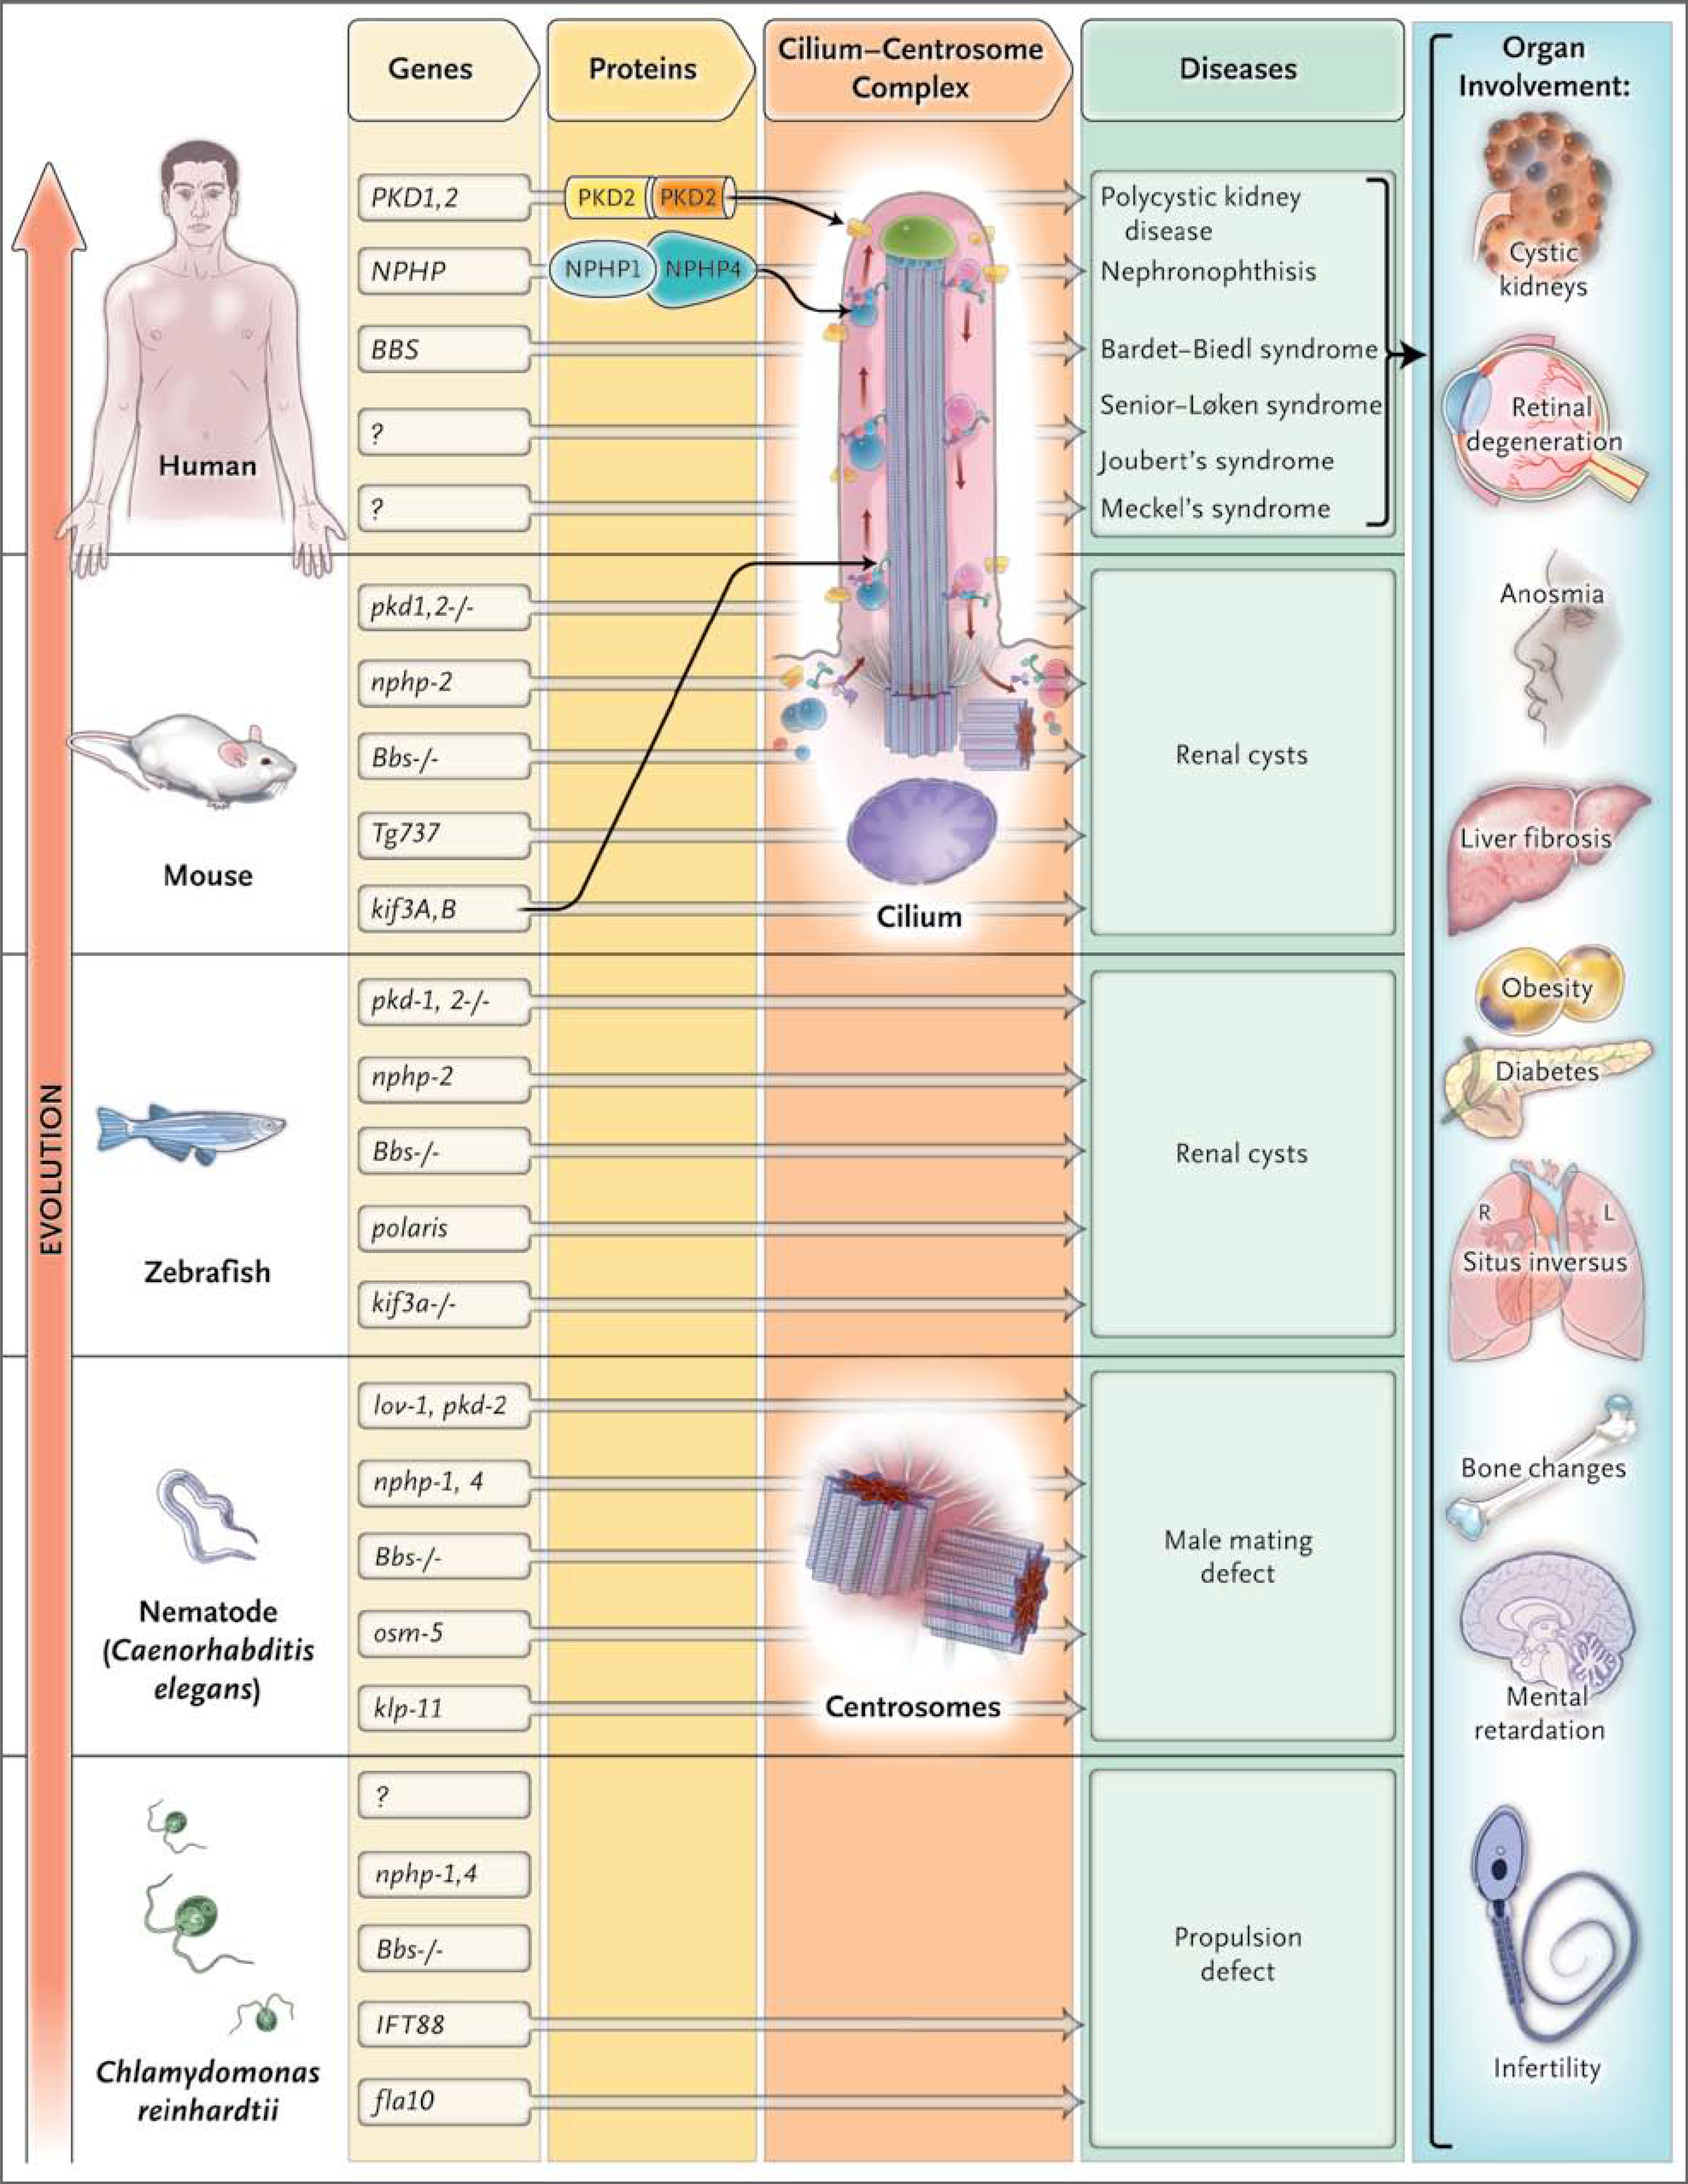
\includegraphics[width=\textwidth]{fig2-9.jpg}
%生成中英双语标题
{\setstretch{1.667}
\bicaption[fig:2.9]{图}{纤毛病及其相关基因\ \citep{Hildebrandt2011}。}{Figure}{Ciliopathies and related genes \citep{Hildebrandt2011}.}
\par}
%结束图片浮动体环境
\end{figure}

纤毛执行着重要的运动、感受、信号转导和分泌等功能,在发育过程中发挥重要作用\
\citep{Bodle2013,Huangfu2003,Warner2013,Corbit2005,Diener2015}。纤毛的形态和功能异常会导致多种纤毛病,从最早发现的卡塔格内综合症\footnote{Kartagener's syndrome, KS}\ \citep{Afzelius1976}\ 到初级纤毛运动障碍\footnote{primary ciliary dyskinesia, PCD}、多囊肾病、肾衰
竭\ \citep{Bizet2015}、先天性心脏病\ \citep{Narasimhan2015}、Meckel-Gruber\ 综合
症\ \citep{Dowdle2011,Shaheen2011}、 朱伯特综合症、巴比二氏综合症、比尔特-霍格-杜贝综合征、STAR\ 综合症\ \citep{Guen2016}、神经管缺陷、肝功能紊乱、内脏异位、眼盲\
\citep{Bifari2015}、耳聋、肥胖\ \citep{Mukhopadhyay2013,Omori2015}、癌
症\ \citep{Seeger-Nukpezah2013}\ 及男性不育
等\ \citep{Tobin2009,Cardenas-Rodriguez2013,Luijten2013,Hildebrandt2011,Hildebrandt2007} (图\ref{fig:2.9})。 这是人们持续研究纤毛的主要原因之一。

目前,研究人员已经鉴定出许多纤毛病的致病基因\ \citep{Wheway2015}(图\ \ref{fig:2.9})。这些基因的产物主要是\ IFT\ 蛋白、组成过渡区的结构蛋白和纤毛相关信号通路中的功能蛋白\
\citep{Czarnecki2012,Wheway2015,Bifari2015,Duran2017}(图\ \ref{fig:2.9})。目前的观测结果显示\ IFT-B\ 主要与正向\ IFT\ 相关,而\ IFT-A\ 则主要与反向\ IFT\ 相关。IFT-B\ 的缺陷一般导致没有或仅有极短的鞭毛,而\ IFT-A\ 的缺陷一般引起鞭毛解聚障碍。理论上,IFT\ 复合物\ B\ 中的亚基异常更容易导致纤毛病发生。然而这恰恰与研究人员累积的数据相反。IFT\ 复合物\ A\ 中的亚基缺陷均能导致纤毛病\ \citep{Perrault2015,Duran2017}。然而\ IFT\ 复合物\ B\ 中仅\ IFT172、IFT88、IFT81、IFT80、IFT54、IFT52\ 和\ IFT27\ 在纤毛病患者中检测到突变且
非常罕见\ \citep{Bizet2015,Perrault2015,Bifari2015,Zhang2016}。 一种可能的解释是\ IFT\ 复合物\ B\ 中的亚基异常是胚胎致死性的\ \citep{Perrault2015},我们观察到的现象只是幸存者偏差造成的\
\citep{Mangel1984}。

\section{鞭毛内运输}
\subsection{鞭毛内运输的发现}
1993\ 年,Kozminski\ 在\ Joel Rosenbaum\footnote{https://en.wikipedia.org/wiki/Joel\_Rosenbaum}\ 的实验室利用微分干涉\footnote{differential interference contrast, DIC}显微镜观察衣藻鞭毛时发现了一种不同于纤毛摆动的运动方式\ \citep{Kozminski1993}。他们发现一些颗粒状物质在沿鞭毛作双向运动并将这种现象命名为鞭毛内
运输\ \citep{Kozminski1993}。 IFT\ 的发现标志着纤毛研究中一个新领域的诞生\ \citep{Satir2017}。通过对鞭毛切片进行电镜观察,人们发现在鞭毛膜和外部二联管之间存在一些由电子致密颗粒线性排列组成的火车样结构\ \citep{Kozminski1993}。 这些火车是执行鞭毛内运输的实体。

随后,Iomini\ 等发现正向\ IFT\ 和反向\ IFT\ 的运动速率和频率均有差异,据此他们提出了一个鞭毛内运输的循环模型。在该模型中,IFT\ 被分为四个阶段,第二和第四阶段分别对应正向\ IFT\ 和反向\ IFT。 在第一和第三阶段,IFT\ 复合物在鞭毛基部和顶部发生重塑\ \citep{Iomini2001,Morga2013}。

\subsection{鞭毛内运输复合物的组成}

%开始表格浮动体环境,其中!表示取消严谨限制,h表示在此处插入,t表示在本页或下一页顶部插入
\begin{table}[!ht]
%居中对齐
\centering
%生成中英双语标题
{\setstretch{1.667}
\bicaption[tab:table2.1]{表}{IFT\ 蛋白在几种模式生物中的名
称\ \citep{Taschner2016}。}{Table}{Nomenclature of IFT proteins in several model organisms \citep{Taschner2016}.}
\par}
%更改表格内文字的字号
\small
%开始绘制表格
%开始绘制表格
\resizebox{\textwidth}{!}{%
\begin{tabular}[c]{>{\columncolor{white}}lllllll @{}}
%绘制一条水平线
\toprule
 & & \multicolumn{5}{c}{Alternative name in other organisms (if different)}\\
\cmidrule{3-7}
Complex & General & \tabincell{l}{\textit{Chlamydomonas}\\ \textit{reinhardtii}} & \tabincell{l}{\textit{Trypanosoma}\\ \textit{brucei}} & \tabincell{l}{\textit{Caenorhabditis}\\ \textit{elegans}} & \tabincell{l}{\textit{Danio}\\ \textit{rerio}} & Mammals \\
\midrule
\textbf{IFT-B} &  &  &  &  &  &  \\
IFT-B1 & IFT88 & - & - & OSM-5 & Polaris & Polaris/Tg737 \\
\rowcolor{lightgray} & IFT81 & - & - & - & - & - \\
 & IFT74 & - & - & - & - & - \\
\rowcolor{lightgray} & IFT70 & FAP259 & PIFTB2 & DYF-1 & Fleer & TTC30A/B \\
 & IFT56 & DYF-13 & PIFTC3 & DYF-13 & - & TTC26 \\
\rowcolor{lightgray} & IFT52 & BLD1 & - & OSM-5 & - & NGD5 \\
 & IFT46 & - & - & DYF-6 & - & - \\
\rowcolor{lightgray} & IFT27 & - & - & (Absent) & - & RabL4 \\
 & IFT25 & FAP232 & - & (Absent) & - & HSPB11 \\
\rowcolor{lightgray} & IFT22 & FAP9 & - & IFTA-2 & - & RabL5 \\
IFT-B2 & IFT172 & - & - & OSM-1 & - & SLB \\
\rowcolor{lightgray} & IFT80 &  &  & CHE-2 & - & WDR56 \\
 & IFT57 & - & - & CHE-13 & - & Hippi \\
\rowcolor{lightgray} & IFT54 & FAP116 & - & DYF-11 & Elipsa & Traf3IP1/MIP-T3 \\
 & IFT38 & FAP22 & PIFTA1 & DYF-3 & Qilin & Cluap1 \\
\rowcolor{lightgray} & IFT20 & - & - & - & - & - \\
\textbf{IFT-A} &  &  &  &  &  &  \\
\rowcolor{lightgray} Core & IFT144 & - & - & DYF-2 & - & WDR19 \\
 & IFT140 & - & - & CHE-11 & - & WDTC2 \\
\rowcolor{lightgray} & IFT122 & FAP80 & - & DAF-10 & - & WDR10 \\
Noncore & IFT139 & - & - & - & - & THM1/TTC21B \\
\rowcolor{lightgray} & IFT121 & - & PIFTD4 & IFTA-1 & - & WDR35 \\
 & IFT43 & - & - & - & - & C14ORF179\\
\bottomrule
\multicolumn{7}{l}{FLA, flagellar assembly;}\\
\multicolumn{7}{l}{CHE, chemosensory;}\\
\multicolumn{7}{l}{OSM, osmotic avoidance;}\\
\multicolumn{7}{l}{DYF, dye-filling;}\\
\multicolumn{7}{l}{DAF, dauer-formation;}
%结束绘制表格
\end{tabular}}
%结束表格浮动体环境
\end{table}

1997\ 年,Piperno\ 和\ Mead\ 鉴定了\ IFT\ 复合物中的\ 13\ 种蛋白。1998\ 年,Cole\ 等鉴定了衣藻\ IFT\ 复合物中的\ 15\ 种蛋白并依据它们的分子量大小分别命名为\ p172、p144、p140、p139、p122、p88、p81、p80、p74、p72、p57/55、p52、p46、p27\ 和\ p20\ \citep{Cole1998}。 后来研究人员用\ IFT\ 代替\ p\ 来作为\ IFT\ 蛋白的标准命名。同时,Cole\ 等还发现\ IFT\ 复合物是由两个亚复合物组成并分别命名为复合物\ A\ 和复合物\ B\ \citep{Cole1998}。

随后,研究人员陆续鉴定出一些新的\ IFT\ 蛋白。到目前为止,IFT\ 复合物\ A\ 包含\ IFT144、IFT140、IFT139、IFT122、IFT121\ 和\ IFT43\ 六个亚基\ \citep{Behal2013,Behal2012}。IFT\ 复合物\ B\ 包含\ IFT172、IFT88、IFT81x2、IFT80、IFT74/72、IFT70、IFT57/55、IFT56、IFT54、IFT52、IFT46、IFT38、IFT27、IFT25、IFT22\  和\ IFT20\ 十六个亚基\ \citep{Behal2013,Behal2012,Taschner2016,Taschner2016a}。

IFT\ 蛋白是一类十分保守的蛋白,在果蝇、线虫、布氏锥虫、斑马鱼和小鼠等纤毛生物中均能够找到它们的同源蛋白。
目前已知的属于\ IFT\ 复合物\ A(550 kDa)的蛋白有\ 6\ 个\ \citep{Morga2013}。 除\ IFT43\ 外,其余五个亚基的分子量都超过\ 120 kDa\ \citep{Behal2013}。这使得对它们的研究变得相对困难。IFT\ 复合物\ A\ 亚基的功能缺陷会导致鞭毛形态和功能异常,如在鞭毛顶端形成突起(由\ IFT\ 复合物\ B\ 的累积导致的)、形成短小的鞭毛,部分情况下甚至没有
鞭毛\ \citep{Behal2012}。

IFT\ 复合物\ B(750 kDa)由至少\ 16\ 种蛋白组成\ \citep{Morga2013}。研究表明,随着离子强度的增加,某些亚基会从复合物\ B\ 解离下来\ \citep{Behal2013}。研究人员据此将\ IFT\ 复合物\ B\ 分为核心复合物和外周亚基。然而,后续研究表明外周亚基可以形成独立于核心复合物的稳定复合物。故而核心复合物被命名为\ IFT-B1,外周复合物被命名为\ IFT-B2\
\citep{Taschner2016a,Taschner2016}。IFT-B1\ 包括\
IFT88、IFT81、IFT74/72、IFT70、IFT56、IFT52、IFT46、IFT27、IFT25、IFT22\ \citep{Behal2013}。 IFT-B2\ 包括\ IFT172、IFT80、IFT57、IFT54、IFT38、IFT20\ \citep{Taschner2016a}。需要指出的是,这种分类与各个亚基在复合物\ B\ 中所处的位置无关。IFT-B1\ 与\ IFT-B2\ 之间的连接由\ IFT88、IFT52N、IFT57\ 和\ IFT38\ 介导\ \citep{Taschner2016a}。

%IFT88\ 是核心复合物中最大的一个亚基。它有十个TPR基序,其中三个出现在\ N\ 端,另外七个出现在\ C\ 端。这表明\ IFT88\ 连接了两个蛋白,可能是其他的亚基,也可能是货物或者膜蛋白。酵母双杂交和化学交联实验的结果显示,IFT88、IFT52(281-381)和\ IFT46\ 之间存在相互作用,它们可以形成异源
%三聚体\ \citep{Lucker2010,Taschner2011}。 在衣藻和脊椎动物中,IFT88\ 对鞭毛的形成是必须的。IFT88\ 与人和小鼠中的\ Tg737\ 及线虫中的\ OSM-5\ 同源。OSM-5\ 突变可导致线虫的化学感受神经元的纤毛显著变短。在斑马鱼中,IFT88\ 参与原肠胚和神经胚形成过程中的定向细胞分裂,且这种功能与纤毛
%无关\ \citep{Borovina2013}。此外,在哺乳动物细胞中,IFT88\ 还参与\ G1-S\ 转变及有丝分裂过程中纺锤体方向的调控。
%
%IFT81\ 和\ IFT74/72\ 均含有两个卷曲螺旋结构域,这使得它们可以发生相互作用。研究表明,IFT81\ 可形成同源二聚体,IFT81\ 和\ IFT74/72\ 可形成各含两个\ IFT81\ 和\ IFT74/72\ 的异源四聚体。Bhogaraju\ 等人研究发现\ IFT81\ 和\ IFT74\ 的\ N\ 端共同作用完成微管蛋白的运输。IFT81\ 的\ N\ 端与微管蛋白的球形结构域结合,而\ IFT74\ 的\ N\ 端则与\ $\upbeta$\ 微管蛋白的\ E-hook\ 结合从而增强该亚复合物对微管蛋白的亲和力\ \citep{Bhogaraju2013a}。 然而,在衣藻中利用\ \textit{IFT74}\ 缺失突变体进行的研究表明\ IFT74\ 可能与微管蛋白的运输无关,IFT74\ 的\ N\ 端调控了\ IFT\ 复合物\ A\ 的招募并直接影响\ IFT\ 进入鞭毛的
%频率\ \citep{Brown2015}。 这两个亚基的突变会导致线虫化学感受功能的缺陷,但影响程度远不及其他\ IFT\ 复合物\ B\ 的亚基。
%
%IFT80。在胚胎发育阶段敲除小鼠中的\ IFT80\ 导致短趾且骺板及关节软骨的形成受到影响,这可能是由于纤毛形成受阻且\ Hh、Wnt\ 信号通路被扰乱进而导致关节软骨分化异常造成的\ \citep{Yuan2015}。
%
%IFT70是IFT复合物B中最保守的亚基之一。它含有多个TPR和异戊烯转移酶基序。研究表明,IFT70介导了IFT颗粒和OSM-3 之间的相互作用。但IFT70并不直接与OSM-3发生相互作用。限制性蛋白酶解和pulldown实验证明IFT70与IFT52 (281-381)和IFT46之间均存在直接相互作用,但无法确认IFT70与IFT88之间是否存在相互作用\
%\citep{Taschner2011}。IFT70的缺失会导致鞭毛变短,其他IFT复合物B亚基的表达水平也发生不同程度的下降。
%
%在部分肾衰竭患者的基因组中检测到IFT54(TRAF3IP1)存在突变,然而患者成纤维细胞的纤毛率没有变化(尽管纤毛长度显著增加)\citep{Bizet2015}。进一步研究表明\ IFT54\ 的N端可结合MAP4,后者与微管结合后可增强微管的稳定性\ \citep{Bizet2015,Guo2010}。IFT54\ 的突变导致微管稳定性过强从而引起肾衰竭\ \citep{Bizet2015}。 此外,IFT54 在线虫中的同源蛋白DYF-11可与过渡纤维功能蛋白FBF1相互作用,后者可控制IFT 复合物进入纤毛\ \citep{Wei2013}。然而衣藻中并无MAP4的同源蛋白,CrIFT54可能通过C端与胞质微管结合\ \citep{Zhu2017a}。此外,IFT54的N端含有CH结构域。在体外实验中,该结构域可与MT或tubulin结合而被认为参与微管蛋白的运输。但是,在衣藻中的研究表明IFT54对微管蛋白的运输是非必须的\ \citep{Zhu2017a}。
%
%IFT52由\textit{BLD1}基因编码,该基因的无效突变体基体结构正常,但纤毛膜紧邻过渡区\
%\citep{Brazelton2001}。IFT52 的突变可导致短肋多指综合征,这是一种常见的纤毛病\ \citep{Zhang2016}。 这些研究表明IFT52对纤毛的形成非常重要。序列分析发现在线虫、小鼠和人中均存在IFT52的同源物,这种保守性进一步证明了其功能的重要性\ \citep{Collet1998,Wick1995}。IFT52环绕基体呈马蹄铁形分布,两基体中间无\ IFT52\
%\citep{Deane2001}。免疫电镜实验进一步证明IFT52定位在过渡纤维近细胞膜的区域。这表明过渡纤维可能是IFT 颗粒和货物的锚定位点\ \citep{Deane2001}。IFT52的C端(382-454)与IFT46的C端(188-319)存在直接相互作用\
%\citep{Lucker2010}。此外,IFT52的C 端还介导了两个核心亚复合物之间的连接\ \citep{Taschner2011}。 这些结果表明IFT52 是核心复合物中的关键亚基。
%
%IFT46具有中心体蛋白的典型特征,即磷酸化、含卷曲螺旋结构域和动态无序区\ \citep{Nido2012}。IFT46的无效突变体会导致衣藻形成短的无法运动的鞭毛。这些鞭毛的轴丝中无外部动力臂和内部动力臂且中央管有缺陷。但表达C端的部分抑制突变株的内部动力臂和中央管均正常。这表明IFT46对外部动力蛋白在鞭毛中的运输至关重要\ \citep{Hou2007}。 进一步研究表明这一过程需要ODA16的参与。ODA16通过与IFT46直接相互作用从而协助ODA从细胞体运输至鞭毛\
%\citep{Ahmed2008,Ahmed2005,Taschner2017}。过表达和敲降敲除分析表明IFT46 在脊椎动物纤毛、神经和颅面部发育过程中扮演了重要角色\ \citep{Lee2015,Park2016}。
%
%IFT27是一个Rab亚家族的小GTP酶。然而其与IFT复合物B的结合与它结合GTP还是GDP无关。敲降IFT27会导致细胞分裂受阻,敲除IFT27是致死性的。这一研究结果表明IFT27除了参与鞭毛内运输外还参与细胞周期的调控。蛋白相互作用研究的结果显示IFT27与IFT81 之间存在相互作用\ \citep{Lucker2010}。
%
%IFT25是一个磷蛋白,其磷酸化状态影响其与IFT复合物B的结合。IFT25对体细胞鞭毛的组装时非必需的,但其对小鼠精子鞭毛的形成至关重要\ \citep{Liu2017a}。此外,IFT25在刺猬信号通路中扮演了重要角色。研究表明,IFT25和IFT27 可发生直接相互作用,它们在胞质中以独立的亚复合物存在。Bhogaraju等解析了这一条形亚复合物的晶体结构。他们发现两个蛋白的作用界面在IFT27 的C 端和IFT25 的环区\
%\citep{Bhogaraju2011}。
%
%IFT22也是一个Rab亚家族的小GTP酶。在布氏锥虫中,IFT22对纤毛的形成是必须的。但在线虫中情况并非如此。在衣藻中用RNA干扰敲降IFT22会导致细胞中IFT蛋白表达水平的下降和鞭毛中IFT蛋白含量的增加。这表明IFT22参与了鞭毛中IFT颗粒含量的控制。
%
%IFT20在鞭 毛内运输过程之外也发挥重要作用。IFT20可通过纤毛依赖和非纤毛依赖途径调控颅面骨发育\
%\citep{Noda2016}。其中,纤毛依赖途径与血小板源生长因子受体PDGFRα-Akt信号通路的紊乱有关,非纤毛依赖途径与胶原蛋白从内质网向高尔基体的运输受阻有关\ \citep{Noda2016}。在正常培养条件下,基础自噬通过降解IFT20来控制纤毛形成和纤毛长度。在血清饥饿条件下,IFT20通过运输ATG16L参与诱导型自噬\citep{Pampliega2013}。
%
%除IFT20外,与IFT-B2中的亚基相关的研究较少。IFT172是IFT复合物B中最大的一个亚基,它通过IFT57的钙调蛋白同源结构域松散的结合在IFT-B2上\ \citep{Taschner2016a}。IFT57与IFT38 通过卷曲螺旋结构域直接相互作用\
%\citep{Taschner2016a}。IFT38的钙调蛋白同源结构域则与IFT80结合\ \citep{Taschner2016a}。IFT80/57/38 均能够结合IFT54/20\ \citep{Taschner2016a}。 需要注意的是,IFT-B2中的IFT54也含有钙调蛋白同源结构域,体外实验证明该结构域是复合物B中的另一个微管蛋白结合位点\ \citep{Taschner2016a}。

\subsection{鞭毛内运输复合物的结构}

%开始图片浮动体环境,其中!表示取消严谨限制,h表示在此处插入,t表示在本页或下一页顶部插入
\begin{figure}[htb]
%居中对齐
\centering
%设置图片搜索路径,每个路径用{}括起来
\graphicspath{{figures/}}
%插入图片并设置图片宽度为文本宽度减10mm
\includegraphics[width=\textwidth-60mm]{fig2-10.jpg}
%生成中英双语标题
{\setstretch{1.667}
\bicaption[fig:2.10]{图}{野生型衣藻鞭毛切片中的\ IFT\ 火车\ \citep{Pigino2009}。}{Figure}{TEM micrographs of \textit{in situ} IFT trains in flat-embedded flagella from  wild-type cells of \textit{Chlamydomonas reinhardtii} \citep{Pigino2009}.}
\par}
%结束图片浮动体环境
\end{figure}

IFT\ 复合物由\ IFT-B1、IFT-B2\ 和\ IFT-A\ 组成。其中\ IFT-A\ 中的外周亚基介导了\ IFT-A\ 核心复合物与\ IFT-B\ 之间的相互
作用\ \citep{Toriyama2016}。
2009\ 年,Pietro Lupetti\ 及其同事发现正向\ IFT\ 的长度为\ 700\ $\pm$\ 244 nm\ \citep{Pigino2009}
(图\ \ref{fig:2.10})。 这种长的\ IFT\ 火车实际上由两列火车平行组成,每列火车由颗粒状结构连接而成,其周期约\ 40 nm\ \citep{Pigino2009}。 正向\ IFT\ 沿\ B\ 管运动\ \citep{Pigino2009,Stepanek2016}。 反向\ IFT\ 的长度为\ 251\ $\pm$\ 45.1 nm,周期为\ \SI{16}{\nm},其结构致密,有极性\ \citep{Pigino2009} (图\ref{fig:2.10})。进一步研究表明,每一个微管二联管都是\ IFT\ 的双向二车道铁轨\ \citep{Stepanek2016}。 正向\ IFT\ 沿\ B\ 管从鞭毛基部移动到顶端,反向\ IFT\ 沿\ A\ 管从鞭毛顶端移动到基部\ \citep{Stepanek2016}。 这使得正向\ IFT\ 和反向\ IFT\ 在移动过程中不会出现碰撞。这一独特现象产生的原因可能是\ IFT\ 分子马达可识别\ A\ 管和\ B\ 管上不同的翻译后修饰\ \citep{Stepanek2016}。 也可能是由于在纤毛的基部和顶端存在特定机制可控制分子马达的轨道\
\citep{Stepanek2016}。然而,Pietro Lupetti\ 领导的团队在二零一六年发表的文章中修正了之前关于\ IFT\ 火车的模型\ \citep{Vannuccini2016}。他们在测定鞭毛再生过程中两种火车的相对数量时发现短火车的数量随鞭毛长度的增加而增加\ \citep{Vannuccini2016}。进一步的观测结果显示存在另一种更“致密”的短火车且与\ B\ 管的第七根原丝接触\ \citep{Vannuccini2016}。这表明存在两种类型的正向\ IFT\ 火车且它们的相对数量随纤毛形成的进行而变化\
\citep{Vannuccini2016}。

%开始图片浮动体环境,其中!表示取消严谨限制,h表示在此处插入,t表示在本页或下一页顶部插入
\begin{figure}[htb]
%居中对齐
\centering
%设置图片搜索路径,每个路径用{}括起来
\graphicspath{{figures/}}
%插入图片并设置图片宽度为文本宽度减10mm
\includegraphics[width=\textwidth]{fig2-11.jpg}
%生成中英双语标题
{\setstretch{1.667}
\bicaption[fig:2.11]{图}{两种不同类型的短火车\ \citep{Vannuccini2016}。相比于较宽的一种(A),较窄的短火车(B)有一个指向鞭毛顶端的狭长凸起(黑色三角)。黄绿色结构为微管,红色和蓝色结构为\ IFT\ 火车。标尺代表\ \SI{100}{\nm}。}{Figure}{The two subtypes of short IFT trains \citep{Vannuccini2016}. Compared with the wide short train (A), there is a slender projection pointing toward the flagellar tip (black triangle) in the narrow short train (B). The flavogreen structures are microtubules. The red and blue structures are IFT trains. Scale bar represents \SI{100}{\nm}.}
\par}
%结束图片浮动体环境
\end{figure}

IFT\ 火车由\ IFT\ 复合物组成,IFT\ 复合物包含\ IFT-B1、IFT-B2\ 和\ IFT-A\ 三个亚复合物。在\ IFT-B1 \ 中,IFT88、 IFT70、IFT52\ 和\ IFT46\ 之间存在相互作用
(图\ \ref{fig:2.12}A)\citep{Taschner2014}。 其中\ IFT52/IFT46\ 两个亚基的\ C\ 端紧密结合形成球形结构域与\ IFT81/IFT74\ 相互作用(图\ \ref{fig:2.12}A)\citep{Taschner2014}。后者的\ C\ 端结合了\ IFT27/IFT25,N\ 端则为微管蛋白结合位点\ \citep{Bhogaraju2013a,Bhogaraju2014,Kubo2016}。在早期的研究中,IFT\ 复合物\ B\ 中的亚基被分为核心亚基和外周亚基。然而,最新的研究表明这些外周亚基可以形成稳定的复合物\ IFT-B2,它与核心复合物\ IFT-B1\ 之间的相互作用是由\ IFT88/IFT57/IFT52/IFT38\ 介
导(图\ \ref{fig:2.12}B)\citep{Taschner2016a}。 在\ IFT-B2\ 中,IFT54\ 的\ CH\ 结构域也可结合微管蛋白,而\ IFT38\ 的\ CH\ 结构域结合\ IFT80,IFT57\ 的\ CH\ 结构域则结合\ IFT172\ \citep{Taschner2016a}。 尽管纤毛是十分保守的细胞器,不同物种中\ IFT\ 的组成和结构可能存在微小的差异。在哺乳动物初级纤毛中,IFT56\ 与\ IFT46\ 存在相互作用,而\ IFT70\ 则仅与\ IFT88/IFT52\ 相互
作用(图\ \ref{fig:2.12}C)\citep{Katoh2016}。在外周亚基中,IFT57、IFT38\ 和\ IFT20\ 有形成同源二聚体的趋势\ \citep{Katoh2016}。
%开始图片浮动体环境,其中!表示取消严谨限制,h表示在此处插入,t表示在本页或下一页顶部插入
\begin{figure}[htb!p]
%居中对齐
\centering
%设置图片搜索路径,每个路径用{}括起来
\graphicspath{{figures/}}
%插入图片并设置图片宽度为文本宽度减10mm
\includegraphics[width=\textwidth]{fig2-12.jpg}
%生成中英双语标题
{\setstretch{1.667}
\bicaption[fig:2.12]{图}{IFT\ 复合物\ B\ 的整体构造。(A)衣藻\ IFT-B\ 核心复合物的构
造\ \citep{Taschner2014}。其中\ IFT81\ 和\ IFT74\ 的\ N\ 端组成了微管结合模块负责微管蛋白的鞭毛内运输。(B)衣藻\ IFT-B1\ 与\ IFT-B2\ 的构造\ \citep{Taschner2016a}。图中将\ IFT54\ 的\ CH\ 结构域也标记为可能的围观蛋白/微管结合位点。(C)哺乳动物初级纤毛\ IFT-B\ 的整体构造\ \citep{Katoh2016}。 黑色粗线代表强相互作用,黑色细线代表弱相互作用,灰色曲线代表同源二聚体,灰色方框代表异源二聚体。}{Figure}{Architecture of the IFT-B complex. (A) Architecture of the core complex of IFT-B in \textit{Chlamydomonas} flagella \citep{Taschner2014}. The N terminuses of IFT81 and IFT74 form a tubulin-binding module which is responsible for the IFT of tubulin. (B) Overall architecture of the IFT-B1 and IFT-B2 complex in \textit{Chlamydomonas} flagella \citep{Taschner2016a}. The CH domain of IFT54 is also labeled as putative tubulin or MT binding site. (C) A map of interactions among IFT-B subunits in mammalian cilia \citep{Katoh2016}. Black thick lines represent strong interactions. Black fine lines represent weak interactions. Grey curved lines indicate homodimers. Grey boxes indicate heterodimers.}
\par}
%结束图片浮动体环境
\end{figure}

已鉴定的\ IFT\ 复合物\ A\ 亚基仅有六个,其中\ IFT144/IFT140/IFT122\ 被称为核心复合物,其余三个亚基则为外周亚基(图\ \ref{fig:2.13})。在核心复合物中,IFT122\ 是核心,而\ IFT121\ 则是外周亚基的组织
者\ \citep{Zhu2017}。IFT139\ 和\ IFT43\ 与核心复合物的连接依赖\ IFT121\ 与\ IFT122\ 之间的相互
作用(图\ \ref{fig:2.13})\citep{Behal2012}。在线虫神经元纤毛中,IFT139\ 和\ IFT43\ 在参与\ dynein-2\ 介导的反向\ IFT\ 的过程中存在功能冗余\ \citep{Yi2017}。这种情况是否普遍存在于反向\ IFT\ 有待进一步研究。实验结果表明,IFT43\ 与\ IFT121\ 的\ C\ 端可以发生直接相互
作用\ \citep{Behal2012}。 然而,在整个细胞体中仅有部分\ IFT43\ 与其他\ IFT\ 复合物\ A\ 的亚基聚合在一起,这表明\ IFT43\ 可能还有其他未知的功能\ \citep{Behal2012,Zhu2017}。

%开始图片浮动体环境,其中!表示取消严谨限制,h表示在此处插入,t表示在本页或下一页顶部插入
\begin{figure}[htb]
%居中对齐
\centering
%设置图片搜索路径,每个路径用{}括起来
\graphicspath{{figures/}}
%插入图片并设置图片宽度为文本宽度减10mm
\includegraphics[width=\textwidth-60mm]{fig2-13.jpg}
%生成中英双语标题
{\setstretch{1.667}
\bicaption[fig:2.13]{图}{IFT\ 复合物\ A\ 中各亚基之间的相互作用网络\ \citep{Behal2012}。对突变
体\ \textit{ift121}\ 进行的分析表明\ IFT122、IFT140\ 和\ IFT144\ 组装成异源三聚体形成\ IFT\ 复合物\ A\ 的核心。由于\ IFT121\ 的突变可导致复合物\ A\ 中\ IFT139\ 和\ IFT43\ 的完全缺失,我们认为\ IFT121\ 与二者均存在相互作用。} {Figure}{A map of interactions among IFT-B subunits \citep{Behal2012}. Based on biochemical analysis of the \textit{ift121} mutant, we propose that IFT122, IFT140, and IFT144 assemble to create a heterotrimeric stable core complex. The interactions of IFT121 with both IFT139 and IFT43 are supported by the observation that loss of IFT121 completely removes IFT139 and IFT43 from complex A.}
\par}
%结束图片浮动体环境
\end{figure}

\section{纤毛蛋白定位相关研究}
\subsection{纤毛扩散屏障及纤毛孔复合物}
\subsubsection{纤毛扩散屏障}
纤毛是突出在细胞表面的细胞器,其内部空间与胞质空间是一体的。胞质组分从胞浆进入纤毛是否受到限制是一个重要的问题。换句话说,是否存在纤毛扩散屏障或类似核孔复合物的控制物质进出纤毛的结构?

%开始图片浮动体环境,其中!表示取消严谨限制,h表示在此处插入,t表示在本页或下一页顶部插入
\begin{figure}[htbp!]
%居中对齐
\centering
%设置图片搜索路径,每个路径用{}括起来
\graphicspath{{figures/}}
%插入图片并设置图片宽度为文本宽度减10mm
\includegraphics[width=\textwidth-50mm]{fig2-3.jpg}
%生成中英双语标题
{\setstretch{1.667}
\bicaption[fig:2.3]{图}{纤毛基部分子大小依赖的扩散屏障模型\ \citep{Kee2013}。 纤毛基部存在分子大小依赖的扩散屏障用于控制可溶性蛋白进入纤毛。10 kDa\ 的分子(紫色)能够自由出入纤毛和细胞核,但\ 70 kDa\ 的分子(红色)则受到限制。左上角插入的图片为\ NIH3T3\ 细胞的纤毛,红色为纤毛标记物\ Arl13b,绿色为\ GFPs\ 或串联\ GFPs。 尽管\ GFPs\ 和串联\ GFPs\ 的分子量存在差异,但它们均能够进入纤毛。这可能是由于二者具有相似的分子直径。GFP\ 代表绿色荧光蛋白,NPC\ 代表核孔复合物。}{Figure}{Model of the size-dependent diffusion barrier at the base of the cilium
\citep{Kee2013}. The base of the cilium contains a size-dependent barrier to entry of soluble proteins. Molecules that are 10 kDa (purple) can enter both the cilium and nucleus but 70 kDa (red) molecules are restricted from both compartments. Insets shows fluorescence micrographs of the cilia of NIH3T3 cells co-expressing monomeric GFP (1x) or tandem (2x or 3x) GFPs together with Arl13b (red) to mark the ciliary compartment. Despite the difference in molecular weight, monomeric and tandem fluorescent protein constructs can enter the ciliary compartment, presumably due to their similar diameters. GFP, green fluorescent protein; NPC, nuclear pore complexes.}
\par}
%结束图片浮动体环境
\end{figure}

Calvert\ 及其同事发现爪蟾感光细胞的连接纤毛(等同于常规纤毛的转变区)不能有效阻止绿色荧光蛋白在内节和外节之间扩散\ \citep{Calvert2010}(图\ \ref{fig:2.3})。进一步研究发现串联绿色荧光蛋白(2x 和3x)也能够通过连接纤毛自由扩散\
\citep{Najafi2012}。 据此,Calvert\
等人认为纤毛基部不存在控制物质出入的扩散屏障(至少对小于\ 80 kDa\ 的蛋白来
说是这样)\citep{Najafi2012}。

然而在哺乳动物细胞初级纤毛上的研究却得出了相反的结论。研究人员将不同分子量的荧光葡聚糖注射到细胞内并观察它们的运动\ \citep{Kee2012}。结果显示小于\ 10 kDa\ 的荧光葡聚糖能够进入细胞核和纤毛,而\ 40-70 kDa\ 的荧光葡聚糖却无法进入\ \citep{Kee2012}。使用荧光标记的可溶性蛋白进行的实验也获得了同样的结果\ \citep{Kee2013}。 这些研究表明大于\ 50 kDa\ 的蛋白无法通过自由扩散进入纤毛,它们的运动受到纤毛扩散屏障的限制\ \citep{Kee2013}。

这些矛盾出现的可能原因是由于在爪蟾中使用的串联绿色荧光蛋白是线性的,而在初级纤毛中使用的葡聚糖和可溶性蛋白是球形的\ \citep{Kee2013}。这意味着纤毛扩散屏障对出入的蛋白的大小和空间结构均存在限制。这一假说已被相关研究证实\ \citep{Kee2013,Lin2013}。总之,纤毛基部存在基于分子大小的扩散屏障,它能有效控制物质出入纤毛
(图\ \ref{fig:2.3})。

\subsubsection{纤毛孔复合物}
纤毛扩散屏障的分子组成是什么呢?核孔蛋白是组成核孔复合物的一类蛋白,研究表明某些核孔蛋白定位在初级纤毛基部形成纤毛孔复合物(ciliary pore complex, CPC)\ \citep{Kee2012,Diener2015}。分子马达\ KIF17\ 进入纤毛依赖这些核孔蛋白的作
用\ \citep{Kee2012}。 这表明纤毛扩散屏障和核孔共享某些分子组分。然而纤毛孔复合物在组成上与核孔复合物可能并非完全一致。这是因为某些关键的核孔蛋白并未出现在纤毛基部,比如核篮亚复合物中的负责细胞核特异性平台形成的核孔蛋白和将\ NPC\
锚定在核膜上的跨膜核孔蛋白\ \citep{Kee2012}。尽管后者的功能可以由纤毛基部的\ NPHK/MKS\ 复合物执行\ \citep{Garcia-Gonzalo2012},这些差异表明\ CPC\ 可能使用了与\ NPC\ 不完全相同的结构蛋白和控制机制\ \citep{Kee2012}。

%开始图片浮动体环境,其中!表示取消严谨限制,h表示在此处插入,t表示在本页或下一页顶部插入
\begin{figure}[htb!]
%居中对齐
\centering
%设置图片搜索路径,每个路径用{}括起来
\graphicspath{{figures/}}
%插入图片并设置图片宽度为文本宽度减10mm
\includegraphics[width=\textwidth]{fig2-4.jpg}
%生成中英双语标题
{\setstretch{1.667}
\bicaption[fig:2.4]{图}{纤毛和细胞核中的核孔蛋白。核孔复合物由一系列的核孔蛋白组成,其中部分核孔蛋白也定位在纤毛基体形成纤毛孔复合物\ \citep{Kee2013}。图中展示了纤毛孔复合物两种可能的结构。(A)核孔蛋白在纤毛基部形成一个大的纤毛孔,轴丝从纤毛孔的中央突出延伸。(B)核孔蛋白在\ Y-links\ 之间形成九个纤毛孔。(C)梨形四膜虫纤毛基体的电镜照片显示在轴丝外围有九个孔
状结构\ \citep{Ounjai2013}。}{Figure}{Nucleoporins in cilia and nuclei. Nuclear pore complexes contain nucleoporin proteins that assemble into subcomplexes \citep{Kee2013}. Some nucleoporin subcomplexes also localize to the transition zone where they are postulated to form a ciliary pore complex. Two possible structural configurations of the nucleoporins at the base of the cilium are presented. (A) Model in which nucleoporins assemble into one large pore at the base of the cilium with the axoneme protruding through the middle of the pore. (B) Model in which nucleoporins assemble into nine pores at the base of the cilium with each pore positioned between the Y-links. (C) Electron cryotomography analysis of isolated basal body structures from the protist \textit{Tetrahymena pyriformis} indicates nine pore structures adjacent to the microtubule axonemes
\citep{Ounjai2013}.}
\par}
%结束图片浮动体环境
\end{figure}

关于\ CPC\ 的另一个重要问题与其整体结构有关。每一个\ NPC\ 都具有典型的\ 8\ 次旋转对称
结构\ \citep{Alber2007},而纤毛确是\ 9+(0)\ 或\ 9+(2)\ 结构\ \citep{Czarnecki2012}。由于我们对核孔蛋白如何在纤毛基部组装形成\ CPC\ 一无所知,这种对称性的差异是否具有重要意义也
不得而知\ \citep{Kee2013}。 一种可能性是核孔蛋白在纤毛基部形成一个大孔,轴丝从孔中穿过(图\ref{fig:2.4})。这样的纤毛孔具有\ 9\ 次旋转对称结构\ \citep{Kee2013}。另一种可能性是在\ Y\ 型连接结构中间有九个纤毛孔(图\ \ref{fig:2.4}),这样的纤毛孔将具有核孔的八次旋转对称结构\ \citep{Kee2013}。 以嗜热四膜虫纤毛为对象进行的研究支持后一种假说\
\citep{Ounjai2013}。研究人员在嗜热四膜虫鞭毛基体中观察到九个靠近轴丝二联管的孔状结构,其直径约\ 53 nm\
\citep{Ounjai2013}。 这与核孔的直径非常接近\ \citep{Beck2004}。此外,研究人员还从分离的基体中鉴定到参与核- 胞质转运的蛋白如\ Ran\
和跨膜核孔蛋白\ NDC-1\ \citep{Ounjai2013}。这些结果进一步表明\ CPC\ 与\ NPC\ 之间存在相似性。

\subsection{纤毛定位序列}
纤毛中的结构和功能蛋白如何被纤毛蛋白运输系统识别并招募到纤毛呢?对纤毛蛋白的研究显示存在特殊的信号序列即纤毛定位序列(ciliary targeting sequence, CTS)将它们靶定到纤毛\ \citep{Malicki2014}。在跨膜蛋白中,CTS\
一般出现在膜的胞质侧(无论是在胞内囊泡还是在纤毛膜上)\citep{Malicki2014}。CTS\ 一般在蛋白的\ C
\ 端,极少出现在\ N\
端,但有时会出现在多重跨膜蛋白的胞内环上\ \citep{Laird2015}。CTS\ 具有多样性,这意味着它们会与不同的运输系统互作\ \citep{Malicki2014}。研究表明,多个信号通路参与了蛋白的纤毛定位。尽管到目前为止大多数\ CTS\ 的结合对象仍然未知,但对纤毛定位序列的研究已经取得了一系列成果并将持续产生有价值的信息。

\subsubsection{RVxP\ 基序}
最常见的\ CTS\ 是\ RVxP\ 基序,目前只在跨膜蛋白和膜相关蛋白中鉴定到,比如\ G\ 蛋白偶联受体、多囊蛋白\ 2、 环核苷酸 门控离子通道蛋白\ CNGB1b、钠钾腺苷三磷酸酶和视黄醇脱氢酶等\
\citep{Laird2015,Geng2006,Jenkins2006,Michalakis2006}。 其中多囊蛋白\ 2\
的\ RVxP\
基序位于\ N\
端,包含该基序的\ N\
端可将人转铁蛋白受体\ hTFR\ 定位到纤毛\ \citep{Geng2006}。

在实验条件下,RVxP\ 基序通常是蛋白靶定到纤毛所必须的,其突变可破坏蛋白的纤毛定位。以人视杆细胞视蛋白为例,其\ RVxP\ 基序的突变可导致视网膜光受体细胞损伤,这是由视蛋白在细胞体中的异位累积导致的\ \citep{Tam2000}。然而,并非所有纤毛蛋白\ C\ 端的\ RVxP\ 基序都是有功能的。比如纤毛肌醇多聚磷酸磷酸酶\ Inpp5e\ 的\ C\ 端\ RVxP\ 基序突变并不影响其纤毛定位。

视蛋白的\ RVxP\ 基序是其靶定到纤毛所必须的,但其他特征序列的存在也必不可少\ \citep{Tam2000}。视蛋白\ C\ 端\ 44\ 个氨基酸残基组成的多肽(视蛋白\ C44)含有\ RVxP\ 基序,它可以将外源蛋白如\ GFP\ 靶定到纤毛。这依赖视蛋白\ C44\ 与膜相互作用,而这与两个相邻的半胱氨酸残基的棕榈酰化有关。它们的缺失将造成视蛋白无法定位到纤毛,且其表型比\ RVxP\ 基序的突变导致的更严重。这些研究表明在光受体细胞中与膜相互作用对蛋白靶定到纤毛至关重要\ \citep{Laird2015}。
多个研究小组通过蛋白质组学的方法鉴定了一些与视蛋白\ C44\ 相互作用的蛋白。生化分析表明这些蛋白作用于视蛋白纤毛定位过程的不同阶段\ \citep{Tam2000,Laird2015}。其中鸟苷三磷酸酶\ Arf4\ 可以结合视蛋白的\ CTS\ 从而介导囊泡从\ TGN\ 上出芽,这是视蛋白纤毛定位的起始过程。最新的研究表明\ Arf4\ 可以增强\ ASAP1\ 与\ FR\ 模体的结合。这反过来可以起始\ Rab11/Rabin8/Rab8\ 复合物的组装。后者可引发视蛋白转位到纤毛。酵母双杂交筛选显示视蛋白的\ C\ 端与胞质动力蛋白存在直接相互作用,研究人员据此推测视蛋白的纤毛定位是依赖微管的。

嗅觉感受神经元纤毛上的环核苷酸门控离子通道蛋白\ CNGB1b\ 的\ C\ 端也含有\ RVxP\ 基序\ \citep{Jenkins2006}。 该蛋白对环核苷酸门控离子通道复合物的纤毛定位是必须的\ \citep{Jenkins2009,Michalakis2006}。 进一步研究发现胞内分选蛋白\ PACS-1\
通过直接结合\ CNGB1b\ 并决定其纤毛定位\ \citep{Jenkins2009}。二者的相互作用依赖丝氨酸/苏氨酸蛋白激酶\ CK2\ 对它们的磷酸化修饰\ \citep{Jenkins2009}。

\subsubsection{FR\ 基序及\ I3-CTS}
除了\ RVxP\ 基序和棕榈酰化的残基外,视蛋白\ C44\ 还含有\ FR\ 基序(其功能暂时没有被证实)。该基序最早在线虫嗅觉\ G\ 蛋白偶联受体\ ODR-10\ 上发现\ \citep{Dwyer2001},其他\ G\ 蛋白偶联受体的\ C\ 端也有该基序。它含有一个疏水氨基酸残基和一个碱性氨基酸残基。FR\ 基序的突变可导致\ ODR-10\ 和\ Smoothened (Smo)\ 无法靶定到纤毛\ \citep{Dwyer2001}。除\ RVxP\ 基序外,许多\ G\ 蛋白偶联受体在它们的第三个胞内环上有纤毛定位序列(I3-CTS)\citep{Berbari2008}。比如生长抑素受体\ SSTR3\ 在该区域含有\ Ax[S/A]xQ\ 基序\ \citep{Berbari2008}。大鼠中枢神经系统中的其他五个生长抑素受体没有该基序,它们也不定位在纤毛。结构域嵌合实验表明\ I3-CTS\ 基序具有重要作用。含有\ SSTR3\ 的\ I3-CTS\ 的\ SSTR5\ 可以定位到纤
毛\ \citep{Berbari2008}。Ax[S/A]xQ\ 基序的突变可破坏该嵌合蛋白的纤毛定位。同样的结论在血清素受体\ HTR6\ 和黑色素浓集激素受体\ MCHR1\
上也得到证实\ \citep{Berbari2008}。然而,并非所有的\ I3-CTS\ 都具有关联。如神经肽\ Y\ 受体\ NPY2R\ 的两个\ I3-CTS\ 与\ SSTR3\ 的就没有相似性。

与视蛋白不同,GPCR\ 的纤毛定位依赖\ I3-CTS,其功能的实现可能由\ BBS\ 蛋白复合体
介导\ \citep{Berbari2008a}。 在小鼠中敲除\ BBS2\ 和\ BBS4\ 可破坏\ SSTR3\ 和\ MCHR1\ 的纤毛定位\ \citep{Berbari2008a}。同样,在培养的细胞中干扰\ BBS3\ 和\ BBS4\ 会影响含有\ SSTR3 I3-CTS\ 的嵌合跨膜蛋白的纤毛定位\ \citep{Berbari2008a}。 在蛋白相互作用的研究中,SSTR3\ 的\ I3-CTS\ 可以“捕获”所有检测的\ BBSome\ 亚基,而多巴胺受体\ 1\ 则与\ BBS5\ 存在直接相互作用\ \citep{Berbari2008a}。总而言之,I3-CTS\ 的功能可能是使\ GPCR\ 与\ BBS\ 蛋白形成的膜外壳连成一体\ \citep{Berbari2008a}。

除\ BBS\ 蛋白外,肥胖相关蛋白\ TULP3\ 和\ IFT\ 复合物\ A\ 对\ SSTR3\ 和\ MCHR1\ 的纤毛定位也有贡献。TULP3\ 依赖其\ N\ 端与\ IFT\ 复合物\ A\ 发生相互作用\ \citep{Mukhopadhyay2010}。而\ IFT\ 复合物\ A\ 和\ TULP3\ 又反过来共同调控了\ SSTR3\ 和\ MCHR1\ 的纤毛定位\ \citep{Mukhopadhyay2010}。 其中,TULP3\ 与\ IFT\ 复合物\ A\ 及磷脂酰肌醇的结合对调控功能的发挥是必须的\
\citep{Mukhopadhyay2010}。

理论上,不同纤毛定位序列通过不同的途径发挥作用。然而这些通路的上游可能是同种因子,比如肥胖相关蛋白\ Tubby。 尽管视蛋白和\ GPCRs\ 的\ CTS\ 存在差异,肥胖相关蛋白\ Tubby\ 却对视蛋白、生长抑素受体\ SSTR3\ 和黑色素浓集激素受体\ MCHR1\ 的纤毛定位均起到调控作用\ \citep{Sun2012}。在\ tubby\ 突变小鼠的视网膜中,视蛋白无法完全穿过连接纤毛到达外段\
\citep{Sun2012}。 而\ SSTR3\ 和\ MCHR1\ 则无法正确定位到大脑神经元的初级纤毛中发挥功能\citep{Sun2012}。

\subsubsection{核定位信号}
研究表明纤毛扩散屏障与核孔复合物之间存在一定的相似性\ \citep{Huang2010}。研究人员将这种类似核孔复合物的结构称之为纤毛孔复合物\ \citep{Kee2013}。这意味着核定位信号(nuclear localization signal, NLS)及相关蛋白可能同时也参与蛋白的纤毛定位\ \citep{Huang2010}。

KIF17\ 是一种正向\ IFT\ 分子马达,正常情况下它定位在纤毛顶端。其\ C\ 端的\ CTS\ 是一连串碱性氨基酸残基组成的多肽,与经典核定位信号存在相似性\ \citep{Dishinger2010}。缺失该\ CTS\ 的\ KIF17\ 无法定位到纤毛。该\ CTS\ 在单独表达的情况下可以定位在细胞核和纤毛。进一步的研究表明\ KIF17\ 的\ CTS\ 通过与\ importin-$\upbeta$2\ 相互作用发挥纤毛定位的功能\
\citep{Dishinger2010}。

视网膜色素\ RP2\ 是一种脂锚定外周膜蛋白\ \citep{Hurd2011}。其氨基酸序列中含有经典及非经典\ NLS。 突变分析发现\ RP2\ 的非经典\ NLS\ 对其纤毛定位至关重要\ \citep{Hurd2011}。该非经典\ NLS\ 通过结合\ importin-$\upbeta$2\ 介导\ RP2\ 通过纤毛孔复合物\
\citep{Hurd2011}。 电压门控性钾离子通道蛋白\ Kv10.1\ 定位在中心体和纤毛膜上调控纤毛解聚,其\ C\ 端含有\ NLS\
\citep{Sanchez2016,Chen2011}。研究表明该\ NLS\ 对\ Kv10.1\ 的纤毛定位至关重要\
\citep{Sanchez2016}。此外,importin-$\upbeta$1\ 被发现能够与纤毛膜蛋白\ Crumbs\ 结合\ \citep{Fan2007}。 然而它们之间的相互作用是否调控了\ Crumbs\ 的纤毛定位还有待进一步研究\citep{Fan2007}。

\subsubsection{类泛素化修饰}
由于调控蛋白进入细胞核和纤毛的结构存在相似之处,控制蛋白入核的其他机制很可能在蛋白进入纤毛的过程中也发挥作用。类泛素化修饰\ SUMOylation\ 是除\ NLS\ 之外的一种广泛存在的控制蛋白入核的方式\
\citep{Zhang2002,Chen2006}。SUMO\footnote{small ubiquitin-related modifier}\ 是一类重要的类泛素蛋白,其三维结构及生化修饰过程与泛素类似,但这两类蛋白质修饰的生物学意义却不尽相同\ \citep{Hay2005}。 研究表明这种翻译后修饰在腺苷酸环化酶\ AC3\
进入纤毛的过程中发挥重要作用\ \citep{McIntyre2015}。腺苷酸环化酶\ AC3\ 定位在神经元纤毛的膜上,常被用作神经元纤毛标记蛋白\ \citep{Bishop2007}。对\ AC3\ 的生物信息学分析显示其含有保守的类泛素化基序
\ \citep{McIntyre2015}。 进一步研究表明\ AC3\ 是类泛素化蛋白的底物\ \citep{McIntyre2015}。 抑制类泛素化修饰系统不影响纤毛的形成与维持,但\ AC3\
无法定位在纤毛\ \citep{McIntyre2015}。同样的,类泛素化基序突变的\ AC3\
也无法定位到纤毛\ \citep{McIntyre2015}。 这些结果表明类泛素化修饰对\ AC3\ 的纤毛定位非常重要。然而将\ AC3\
的类泛素化基序连接到非纤毛蛋白\ ANO1\
上并不能使\ ANO1\
定位到纤毛\ \citep{McIntyre2015}。这表明类泛素化修饰是\ AC3\
定位到纤毛的必要但不充分条件。

\subsection{IFT\ 蛋白基体定位相关研究}
\subsubsection{调控\ IFT\ 蛋白基体定位的蛋白质}
目前关于\ IFT\ 蛋白基体定位机制的研究较少。大部分研究集中在\ IFT20\ 上。然而,IFT20\ 大量聚集在高尔基体。该蛋白除参与纤毛的组装与解聚外还与蛋白转运等密切相关\ \citep{Follit2006,Follit2008}。 因而相关研究可能无法拓展到其他\ IFT\ 蛋白上。

免疫共沉淀实验显示\ IFT20\ 与\ CCDC41(Cep83)之间存在相互作用,CCDC41\ 对\ IFT20\ 被招募到中心体是必须的\
\citep{Joo2013}。此外,IFT20\ 离开顺式高尔基体膜囊受\ VPS15\ 和\ GM130\ 的调控\ \citep{Stoetzel2016}。VPS15\ 的突变导致\ IFT20\
无法有效从顺式高尔基体上释放从而造成纤毛变短\ \citep{Stoetzel2016}。然而,CCDC41\
并没有参与\ IFT88\
富集在中心体的过程\ \citep{Joo2013}。 由于\ IFT20\
和\ CCDC41\
参与纤毛囊泡的锚定而不是轴丝的延伸,故\ CCDC41\ 对\ IFT\
蛋白基体定位的调控可能不存在普遍性。与之类似,另一个与初级纤毛囊泡形成有关的蛋白\ EHD1\
对\ IFT20\
被招募到母中心粒远端也可能没有普遍性\ \citep{Lu2015,Naslavsky2011}。

在初级纤毛中,C2cd3\ 可以招募\ CCDC41、Cep164、TTBK2、IFT88\ 和\ IFT52\ 定位到母中心粒远端\
\citep{Ye2014,Cajanek2014},而\ TTBK2\ 可以招募\ IFT140\ 和\ IFT88\ 定位到过
渡区\ \citep{Goetz2012,Tsang2013}。OFD1\ 也可以招募\ IFT88\ 定位到基体\ \citep{Singla2010}。由于相关蛋白的抗体和突变体有限,以上关于\ IFT\ 蛋白基体定位的研究均比较零散。2016\ 年,Toriyama\ 及其同事发现纤毛病相关蛋白\ Jbts17(也被称为C5orf42)定位在基体,它可以招募\ CPLANE(包括Intu、Rsg1、Wdpcp、Jbts17\ 和\ Fuz)的其他成员定位到基体\
\citep{Toriyama2016}。CPLANE\
可以进一步招募\ IFT\ 复合物\ A\ 中的外周亚基定位到基体\ \citep{Toriyama2016}。2017\ 年,Yeyati\ 等人发现组蛋白赖氨酸去甲基化酶\ KDM3A\ 可通过调控肌动蛋白细胞骨架间接影响\ IFT\ 蛋白的基体和纤毛定
位\ \citep{Yeyati2017}。然而,目前还没有鉴定到直接影响\ IFT-A\ 核心亚基以及\ IFT-B\ 亚基基体定位的蛋白。

\subsubsection{IFT\ 蛋白基体定位相关模型}
纤毛内部无蛋白合成系统,纤毛延伸过程中其所需的前体蛋白均来自细胞体。研究表明,细胞体中存在纤毛前体蛋白的库\ \citep{Fowkes1998,Rosenbaum1969}。在衣藻中,这个库足够形成两根长度减半的鞭毛\
\citep{Rosenbaum1969}。 大部分纤毛蛋白在库中不是单个的存在,而是预组装形成复合物,如\ ODA\  \citep{Fowkes1998}、IDA\ \citep{Piperno1997}和\ RS\ \citep{Qin2004}。结合其他鞭毛蛋白基体定位机制的研究,“预组装-定位”可能是鞭毛蛋白基体定位的主要模式。

%开始图片浮动体环境,其中!表示取消严谨限制,h表示在此处插入,t表示在本页或下一页顶部插入
\begin{figure}[hbt]
%居中对齐
\centering
%设置图片搜索路径,每个路径用{}括起来
\graphicspath{{figures/}}
%插入图片并设置图片宽度为文本宽度减10mm
\includegraphics[width=\textwidth-40mm]{fig2-14.jpg}
%生成中英双语标题
{\setstretch{1.667}
\bicaption[fig:2.14]{图}{IFT-B\ 核心复合物体内组装的假想模型\ \citep{Lucker2010}。
IFT46、IFT52\ 和\ IFT88\ 形成异源三聚体并与\ IFT81、IFT74/72\ 异源四聚体和\ IFT27/25\ 异源二聚体组装。这些亚基或亚复合物组装的具体顺序是未知的。} {Figure}{Hypothetical model of \textit{in vivo} assembly of the IFT complex B core \citep{Lucker2010}. IFT46, IFT52, and IFT88 form a ternary complex prior to assembly with the IFT81, IFT74/72 tetramer and IFT27/25 heterodimer. The actual order in which these and additional subunits assemble onto the core is unknown.}
\par}
%结束图片浮动体环境
\end{figure}

%开始图片浮动体环境,其中!表示取消严谨限制,h表示在此处插入,t表示在本页或下一页顶部插入
\begin{figure}[htbp]
%居中对齐
\centering
%设置图片搜索路径,每个路径用{}括起来
\graphicspath{{figures/}}
%插入图片并设置图片宽度为文本宽度减10mm
\includegraphics[width=\textwidth-85mm]{fig2-15.jpg}
%生成中英双语标题
{\setstretch{1.667}
\bicaption[fig:2.15]{图}{IFT-B的层级组装和基体定位模型\ \citep{Richey2012}。首先,
亚复合物\ IFT88/70/52/46\ 和\ IFT27/25\ 结合形成\ IFT88/70/52/46/27/25。该过程依赖\ IFT52。随后,IFT81\ 和\ IFT74\ 结合\ IFT88/70/52/46/27/25\ 形成\ IFT88/70/52/46/27/25/81/74。此步骤需要\ IFT46\ 的参与。最后,外周亚基组装到核心复合物上形成完整的复合物\ B。IFT88\ 对核心复合物的形成是非必须的,但它介导了外周亚基与核心复合物之间的结合。核心复合物的组装发生在基体远端,从远端转位到
过渡纤维依赖\ IFT88\ 及外周亚基的正常结合。} {Figure}{Sequential assembly and basal body localization of complex B \citep{Richey2012}. First, the subcomplexes IFT88/70/52/46 and IFT27/25 binds to form IFT88/70/52/46/27/25, and the binding is dependent on IFT52. Second, IFT74 and IFT81 assemble onto IFT88/70/52/46/27/25 to form IFT88/70/52/46/27/25/81/74. This step is assisted by IFT46. Lastly, the peripheral proteins assemble onto the complex B core to form an intact complex B. IFT88 is essential for mediating the binding of peripheral proteins to the B core. All the assembly steps involved in forming complex B core may occur at the proximal end of the basal bodies. The translocation from the proximal end of the basal body to the transition fibers dependents on the presence of IFT88 and proper association of peripheral proteins.}
\par}
%结束图片浮动体环境
\end{figure}

基于对\ IFT\ 复合物各亚基生化、遗传、定位和相互作用等方面的研究,\citet{Lucker2010}\ 提出了\ IFT\ 复合物\ B\ 的层级组装模型(图\ \ref{fig:2.14})。在该模型中,IFT88、IFT52\ 和\ IFT46\ 形成异源三聚体,IFT81\ 和\ IFT74/72\ 形成异源四聚体,IFT27\ 和\ IFT25\ 形成异源二聚体。这三个独立的亚复合物与其他亚基相互作用形成\ IFT\ 复合物\ B\ 的核心复合物。外周亚基随后与该核心相互作用形成完整的\ IFT\ 复合物\ B\ \citep{Lucker2010}。随
后,\citet{Richey2012}\ 基于对相关突变体进行的分析也提出了类似的模型(图\ \ref{fig:2.15})。他们认为\ IFT88、IFT70、IFT52\ 和\ IFT46\ 形成异源四聚体。该异源四聚体随后结合\ IFT27/IFT25\ 和\ IFT81/IFT74。通过以上步骤形成的\ IFT-B\ 核心复合物随后结合外周亚基形成完整的\ IFT-B\ \citep{Richey2012}。这两个模型虽然能够解释部分\ IFT\ 基因突变体的表型差异,但相关证据不够充分,需要进一步验证和研究。
%开始图片浮动体环境,其中!表示取消严谨限制,h表示在此处插入,t表示在本页或下一页顶部插入
\begin{figure}[htb!]
%居中对齐
\centering
%设置图片搜索路径,每个路径用{}括起来
\graphicspath{{figures/}}
%插入图片并设置图片宽度为文本宽度减10mm
\includegraphics[width=\textwidth-30mm]{fig2-16.jpg}
%生成中英双语标题
{\setstretch{1.667}
\bicaption[fig:2.16]{图}{IFT\ 蛋白之间及\ IFT\ 蛋白与分子马达或货物之间的相互作
用\ \citep{Taschner2016}。MT\ 为微管,\textit{C. reinhardtii}\ 为莱茵衣藻,\textit{C. elegans}\ 为线虫。}{Figure}{Interactions within IFT proteins and interaction between IFT proteins/complexes and ciliary motor/cargo proteins \citep{Taschner2016}. MT, Microtubule; \textit{C. reinhardtii}, \textit{Chlamydomonas reinhardtii}; \textit{C. elegans}, \textit{Caenorhabditis elegans}.}
\par}
%结束图片浮动体环境
\end{figure}

近年来,Esben Lorentzen\ 教授率领的团队陆续解析了\ IFT-B\ 复合物中部分亚基及其货物的晶体结构\ (图\ \ref{fig:2.16}),如IFT25/27、IFT70/52、IFT52/46、IFT81/74/tubulin\ 和\ IFT46/ODA16 \citep{Bhogaraju2011,Taschner2014,Taschner2017,Bhogaraju2013a,Bhogaraju2014}。 同时他们还依据蛋白纯化结果将\ IFT-B\ 分为\ IFT-B1\ 和\ IFT-B2\ 两个子复合物\ (图\ \ref{fig:2.14})\citep{Taschner2016a}。这些研究虽然旨在解析\ IFT-B\ 及其与分子马达和货物的整体结构,但鉴于其与已知体内实验结果的高度吻合\ \citep{Kubo2016,Craft2015,Ahmed2008}。我们认为\ IFT\ 复合物的晶体结构可在一定程度上指导对\ IFT\ 蛋白基体定位的相关研究。然而,体内实验长期以来受到有限的突变体和抗体的制约。此外,研究多亚基复合物组装的方法和手段也很匮乏。

相比于\ IFT-B\ 复合物中的亚基,对\ IFT-A\ 复合物中亚基的基体定位相关研究较少。原因之一是\ IFT-A\ 中的亚基分子量普遍较大。\citet{Brown2015}\ 发现\ IFT-A\ 和\ IFT-B\ 在野生型衣藻的基体共定位。然而,这种共定位在\ \textit{IFT74}\ 的缺失突变体\ \textit{ift74-2}\ 中消失。这一结果表明\ IFT-A\ 和\ IFT-B\ 通过独立的方式定位到基体。在已有的研究中,IFT-A\ 在\ IFT-B\ 亚基的缺失突变体中能够正常定位到基体。反之,IFT-B\ 在\ IFT-A\ 亚基的缺失突变体中也能够正常定位到基体\ \citep{Behal2012,Brown2015,Hou2007,Richey2012}。此外,前面提到的\ CPLANE\ 蛋白能够招募\ IFT-A\ 外周亚基,而非\ IFT-A\ 核心亚基或\ IFT-B\ 定位到基体\ \citep{Toriyama2016}。 这些结果进一步验证了“预组装-定位”模型。

在未来的研究中,我们需要确定到底哪些亚基和货物在定位到基体之前已经预组装成亚
复合物\ \citep{Lechtreck2015,Lechtreck2017,Taschner2016,Fu2016}。同时我们还需要探究这些亚复合物的组装次序。这些研究有助于最终阐明\ IFT\ 蛋白基体定位以及与货物相互作用的机制。这对解析纤毛的组装与解聚机理至关重要。同时,这些研究对调控纤毛形成及纤毛功能和纤毛病的预防与治疗也具有重要的指导意义。
%调入第三章,不要加拓展名tex。
%input和include命令均能够调入子文档,但include会重启一页
\chapter{IFT46定位在基体和纤毛}
\renewcommand{\leftmark}{第三章\quad IFT46定位在基体和纤毛}

\section{引言}
\blindtext

\section{材料与方法}
\subsection{材料}
\Blindtext

\subsection{方法A}
\Blindtext

\subsection{方法B}
\Blindtext

\subsection{方法C}
\Blindtext

\subsection{方法D}
\Blindtext

\section{结果}
\subsection{结果A}
\Blindtext

\subsection{结果B}
\Blindtext

\subsection{结果C}
\Blindtext

\subsection{结果D}
\Blindtext

\section{讨论}
\Blindtext

\section{小结}
\Blindtext
%调入第四章,不要加拓展名tex。
%input和include命令均能够调入子文档,但include会重启一页
\chapter{IFT46基体和纤毛定位序列的鉴定}
\renewcommand{\leftmark}{第四章\quad IFT46基体和纤毛定位序列的鉴定}

\section{引言}
\blindtext

\section{材料与方法}
\subsection{材料}
\Blindtext

\subsection{方法A}
\Blindtext

\subsection{方法B}
\Blindtext

\subsection{方法C}
\Blindtext

\subsection{方法D}
\Blindtext

\section{结果}
\subsection{结果A}
\Blindtext

\subsection{结果B}
\Blindtext

\subsection{结果C}
\Blindtext

\subsection{结果D}
\Blindtext

\section{讨论}
\Blindtext

\section{小结}
\Blindtext
%调入第五章,不要加拓展名tex。
%input和include命令均能够调入子文档,但include会重启一页
%latex提供的标题命令有如下九个。注意部分标题命令仅能在特定文类中使用。
    %\part
    %\chapter (report style only)
    %\section
    %\subsection
    %\subsubsection
    %\paragraph
    %\subparagraph
    %\subsubparagraph (milstd and book-form styles only)
    %\subsubsubparagraph (milstd and book-form styles only)
%标明文档使用的编码方式。UTF-8是Unicode的一种,使用它可以方便的编辑各种语言。如果没有正确设置编码方式,编译带中文的文档会产生 Package CJK Error: Invalid character code这样的错误。手动设置文档编码方式方法如下:document/document settings/format/UTF-8。使用UTF-8 + XeLaTeX排版中文文档是一种完美选择。这里我使用的是PDFTeXify或PDFLaTeX引擎,这样可以一步到位直接生成最后的PDF文件。
% !Mode:: "TeX:UTF-8"
%空行代表重启一个段落。
\chapter{IFT52\ 结合并招募\ IFT46\ 至基体}
%直接在奇数页页眉中显示章标题会多出一些章标题内部编号,这里重新定义\leftmark,后续所有章节都要重新定义
\renewcommand{\leftmark}{第五章\quad IFT52\ 结合并招募\ IFT46\ 至基体}
\section{引言}
在前一章的研究中我们鉴定到了\ IFT46\ 的基体和纤毛定位序列。同时我们发现其定位序列能够与其他\ IFT\ 蛋白相互作用形成复合物从而沿轴丝做双向运动。这暗示我们\ IFT46\ 是在其他\ IFT\ 相关蛋白的帮助下定位到基体。为了找到\ IFT46\ 的上游运载蛋白,我们拟在\ IFT\ 相关蛋白的缺失突变体中表达\ IFT46\ 或\ IFT46-C1。 如果\ IFT46\ 的基体定位不依赖某个\ IFT\ 蛋白,那么\ IFT46\ 应该能够继续定位在基体。否则,IFT46\ 将无法成功定位在基体。

\section{材料与方法}
\subsection{本研究所用仪器、试剂、培养基及溶液}
如未在正文中特别说明,本研究所用仪器、试剂、培养基及溶液信息均列于附录部分。其中,仪器信息列于
第\ \pageref{appen:A}\ 页的附录\ A,试剂信息列于第\ \pageref{appen:B}\ 页的附录\ B,培养基信息列于
第\ \pageref{appen:C}\ 页的附录\ C,溶液信息列于第\ \pageref{appen:D}\ 页的附录\ D。

\subsection{藻细胞株及菌株的培养}
本章实验所用藻株有\ CC-125\index{CC-125}、\textit{ift46-1}\index{\textit{ift46-1}}、\textit{bld1}、\textit{ift122-1}、\textit{ift88 null}、\textit{ift81-2}、\textit{dhc1b null}\ 和\ \textit{fla10-2}。其中\ \textit{ift122-1} \ 和\ \textit{ift81-2}\ 由清华大学的潘俊敏教授馈赠。通过电转化、筛选获得的藻株列于第\
\pageref{appen:E}\ 页的附录\ E。培养条件及方法
参考第\ \pageref{subsec:algae}\ 页\ \ref{subsec:algae}\ 部分。大肠埃希氏菌\index{大肠杆菌}\ DH5$\upalpha$\ 菌株由本实验室保存。培养条件及方法参考第\ \pageref{subsec:algae}\ 页\
\ref{subsec:algae}\ 部分。

\subsection{计算机辅助分析}
\textit{IFT52}\ 的基因组\ DNA\ 及蛋白序列均来源于\ Joint Genome Institute Phytozome 12\footnote{https://phytozome.jgi.doe.gov/pz/portal.html}\ 中的
\ \textit{Chlamydomonas reinhardtiiv} 5.5\ 数据库。嗜热四膜虫\ TtIFT52C/46C\ 的晶体结构文件下载自\ RCSB Protein Data Bank\footnote{http://www.rcsb.org/pdb/home/home.do}(ID:4UZZ)
\citep{Taschner2014}。衣藻\ CrIFT52C/46C\ 的三维结构根据\ TtIFT52C/46C\ 的晶体结构利用\ Phyre2\ 进行模拟产生\ \citep{Kelley2015}。获得的结构文件用\ Protein Workshop
\citep{Moreland2005,Xu2009}\ 进行观察并找出\ IFT52C\ 和\ IFT46C\ 结合界面上关键的疏水残基用于定点突变。

\subsection{分子克隆}
如未作特殊说明,分子克隆所用方法参考第\ \pageref{subsec:melcular cloning}\ 页\
\ref{subsec:melcular cloning}\ 部分和第\ \pageref{subsec:melcular cloning second}\ 页
\ \ref{subsec:melcular cloning second}\ 部分。

%开始图片浮动体环境,其中!表示取消严谨限制,h表示在此处插入,t表示在本页或下一页顶部插入
\begin{figure}[!ht]
%居中对齐
\centering
%设置图片搜索路径,每个路径用{}括起来
\graphicspath{{figures/}}
%插入图片并设置图片宽度为文本宽度减10mm
\includegraphics[width=\textwidth-30mm]{fig5-1.jpg}
%生成中英双语标题
{\setstretch{1.667}
\bicaption[fig:5.1]{图}{In-Fusion\ 同源重组克隆方法示意图。通过\ PCR\ 获得的\ DNA\ 片段和线性化载体被\ In-Fusion\ 重组酶融合成完整载体。图中彩色方框代表重叠的\ 15 bp\ 片段。}{Figure}{Schematic diagram of In-Fusion HD cloning method. PCR-generated sequences and linearized vector are fused together by In-Fusion enzyme. Colored boxes at ends of DNA fragments are 15 bp overlap.}
\par}
%结束图片浮动体环境
\end{figure}

\subsubsection{In-Fusion\ 同源重组克隆}\label{subsubsec:in fusion}
In-Fusion\ 同源重组克隆的原理如图\ \ref{fig:5.1}\ 所示\ \citep{Marsischky2004,Gibson2009}。使用\ In-Fusion HD Cloning Kit (Clontech, Cat\#639636),按表\
\ref{tab:table5.1}\ 加入各试剂后混匀,瞬时离心后\ \SI{50}{\degreeCelsius}\ 反应三十分钟,冰上静置一分钟。将所有的反应产物用于热激转化,转化方法参考第\ \pageref{subsub:heat transformation}\ 页\ \ref{subsub:heat transformation}\ 部分。从平板上挑二十四个单克隆至含有\ \SI{1}{\mL}\ LB\ 液体培养基(含\ \SI{100}{\ug}/\si{\mL}\ 氨苄青霉素)的\ \SI{2}{\mL}\ 离心管中,\SI{37}{\degreeCelsius}\ 培养过夜后进行菌液\ PCR\ 鉴定,引物为\ IFT52seq-F\ 和\ IFT52seq-R。选择三个阳性克隆扩大培养抽提质粒进行酶切验证。

%开始表格浮动体环境,其中!表示取消严谨限制,h表示在此处插入,t表示在本页或下一页顶部插入
\begin{table}[!ht]
%居中对齐
\centering
%生成中英双语标题
{\setstretch{1.667}
\bicaption[tab:table5.1]{表}{In-Fusion\ 同源重组克隆反应体系}{Table}{Reaction system for In-Fusion cloning}
\par}
%更改表格内文字的字号
\small
%开始绘制表格
\begin{tabular*}{\textwidth}[c]{@{\extracolsep{\fill}}lll}
%绘制一条水平线
\toprule
编号\ (Number) & 试剂\ (Reagents)       & 质量或体积\ (Mass or Volume)\\
\midrule
1 & IFT52 promoter                              & \SI{100}{\ng}\\
2 & IFT52C                                      & \SI{100}{\ng}\\
3 & \textit{Nde}I \textit{Sda}I digested pHK470 & \SI{50}{\ng}\\
4 & 5x In-Fusion Enzyme Premix                  & \SI{1}{\uL}\\
5 & ddH$_2$O                                    & To \SI{5}{\uL}\\
\bottomrule
%结束绘制表格
\end{tabular*}
%结束表格浮动体环境
\end{table}

\subsubsection{定点突变}\label{subsubsec:SDM}
使用全式金点突变试剂盒进行定点突变,基本原理如图\
\ref{fig:5.2}\ 所示\
\citep{Higuchi1988,Zheng2004,Ko2005}。具体步骤如下。

(1)使用\ GeneTool Lite\ 设计引物\ SDM-F\ 和\ SDM-R。

(2)使用下列体系进行\ PCR\ 扩增:质粒模板,5 ng;\SI{10}{\micro\nauticalmile}\ SDM-F,1 $\upmu$L;10 $\upmu$M SDM-R,1 $\upmu$L;2xTransStart FastPfu PCR SuperMix,25 $\upmu$L;ddH$_2$O,至\ 50 $\upmu$L。其中质粒模板必须来源于非甲基化缺陷型菌株,如实验室常用的\ DH5$\upalpha$\ 和\ DH10$\upbeta$。PCR \ 反应程序如下:
\SI{95}{\degreeCelsius}\ 预变性五分钟;\SI{95}{\degreeCelsius},二十秒;\SI{60}{\degreeCelsius},二十秒;
\SI{72}{\degreeCelsius},两分钟;循环二十次;\SI{72}{\degreeCelsius}\ 补时延伸十分钟。

(3)向\ PCR\ 产物中加入\ \SI{1}{\uL} DMT\ 酶,混匀后瞬时离心,\SI{37}{\degreeCelsius}\ 孵育一小时。

(4)取\ \SI{5}{\uL} DMT\ 酶消化产物加入到\ \SI{50}{\uL}\ 感受态细胞中进行热激转化,具体步骤参考
第\ \pageref{subsub:heat transformation}\ 页\ \ref{subsub:heat transformation}\ 部分。

(5)取\ \SI{200}{\uL}\ 菌液均匀的涂在抗性平板上,在\ \SI{37}{\degreeCelsius}\ 培养箱中过夜培养。

(6)挑取单克隆接种到含\ 1 mL LB\ 培养基(含\ 100 $\upmu$g/mL\ 的氨苄青霉素)的\ \SI{1.5}{\mL}\ 离心管中培养过夜,取\ \SI{100}{\uL}\ 菌液测序。选择突变成功的单克隆抽提质粒进行后续实验。

%开始图片浮动体环境,其中!表示取消严谨限制,h表示在此处插入,t表示在本页或下一页顶部插入
\begin{figure}[!ht]
%居中对齐
\centering
%设置图片搜索路径,每个路径用{}括起来
\graphicspath{{figures/}}
%插入图片并设置图片宽度为文本宽度减10mm
\includegraphics[width=\textwidth]{fig5-2.jpg}
%生成中英双语标题
{\setstretch{1.667}
\bicaption[fig:5.2]{图}{定点突变原理示意图。首先利用重叠引物通过反向\ PCR\ 扩增获得带突变的质粒。然后用\
\textit{Dpn}I\ 消化甲基化和半甲基化的模板。最后将消化后的产物转化至\ DMT\ 感受态细胞中完成缺口修复。} {Figure}{Overview of the TRANS Fast Site-directed Mutagenesis System. The first step is to obtain mutated plasmid DNA using overlapped primers through reverse PCR. Then, the methylated and semi-methylated plasmid DNA in the amplification products are digested with \textit{Dpn}I. Finally, digested-products are transformed into DMT competent cells for nick repair.}
\par}
%结束图片浮动体环境
\end{figure}

\subsubsection{载体构建}
为了拯救\ \textit{IFT52}\ 的缺失突变体\ \textit{bld1},我们构建了\ pHK250(表达\ IFT52::YFP\ 和巴龙霉素抗性基因)、pHK268 (表达\ IFT52::YFP\ 和潮霉素抗性基因)和\ pHK409(表达\ IFT52::3HA\ 和巴龙霉素抗性基因)。
以\ CC-503\ 的基因组\ DNA\ 为模板,用引物\ IFT52A-F\ 和\ IFT52B-R\ 扩增\ \textit{IFT52}\ 的基因组\ DNA。 扩增产物经\
\textit{Nde}I/\textit{Eco}RV\ 双酶切后连接到\ \textit{Nde}I/\textit{Eco}RV\ 消化后的\ pHK86\ 或\ pHK266,分别获得\ pHK250\ 和\ pHK268。为了在\ IFT52\ 的\ C\ 端融合\ 3xHA\ 标签,使用寡核苷酸\ HA1、HA2、HA3\ 和\ HA4\ 退火合成\ 3xHA\ 的核酸序列并连接到\ \textit{Eco}RV/\textit{Eco}RI\ 消化后的\ pHK250,由此获得表达\ IFT52::3HA\ 的\ pHK409\
(参考第\ \pageref{subsec:oligoanneal}\ 页\ \ref{subsec:oligoanneal}\ 部分)。

使用\ \textit{Nde}I/\textit{Eco}RV\ 将\ IFT46-C1\ 的编码序列从\ pHK245\ 上切割下来并将其连接到\ \textit{Nde}I/\textit{Eco}RV\ 消化后的\ pHK266\ 中,由此获得表达\ IFT46-C1\ 和潮霉素抗性基因的\ pHK242。 为了破坏\ IFT46-C1\ 和\ IFT52\ 之间的相互作用,我们使用引物\ SDM-F\ 和\ SDM-R\ 对\ pHK242\ 进行了定点突变
(参考第\ \pageref{subsubsec:SDM}\ 页\ \ref{subsubsec:SDM}\ 部分)。由此产生的载体\ pHK267\ 可表达\ IFT46-C1$^{L285E/L286E}$::YFP。

为了构建表达\ YFP::NLS\ 的\ pHK464,我们利用\ \textit{Eco}RV/\textit{Eco}RI\ 双酶切将\ pHK469\ 上的第二个\ \textit{yfp}\ 基因切除并插入\ 4xSV40 NLS。4xSV40 NLS\ 是通过五条寡核苷酸\ 4xNLS-1F、4xNLS-2R、4xNLS-3F、4xNLS-4R\ 和\ 4xNLS-5R\ 退火产生的。以\ pHK464\ 为模板,用引物\ NLS-F\ 和\ NLS-R\ 扩增\ \textit{yfp}-NLS\ 序列。扩增产物经\
\textit{Sma}I/\textit{Eco}RI\ 双酶切后连接到经\ \textit{Eco}RV/\textit{Eco}RI\ 消化后的\ pHK409 \ 中,由此获得\ pHK470。为了构建表达\ IFT52C::YFP::NLS\ 的\ pHK473,我们以\ pHK470\ 为模板,利用引物\ IFT52C-F\ 和\ IFT52C-R\ 进行扩增,扩增产物经纯化后利用\ In-Fusion\ 方法重组克隆(参考第\ \pageref{subsubsec:in fusion}\ 页\ \ref{subsubsec:in fusion}\ 部分)。

\subsubsection{质粒提取}
使用\ Omega\ 去内毒素质粒小提试剂盒进行质粒提取,具体步骤如下。

(1)取\ 1-\SI{5}{\mL}\ 细菌培养物,室温\ \SI{12000}{\g}\ 离心一分钟,尽量吸除上清。

(2)向留有菌体沉淀的离心管中加入\ \SI{250}{\uL}\ Solution I\ (请先检查是否已加入\ RnaseA),使用移液器或涡旋振荡器彻底悬浮细菌细胞沉淀。

(3)向离心管中加入\ \SI{250}{\uL}\ Solution II,温和地上下翻转四至六次使菌体充分裂解。注意混匀一定要温和,以免污染细菌基因\ DNA,此时菌液应变得清亮粘稠,作用时间不要超过五分钟,以免质粒受到破坏。但也不要低于两分钟,以免裂解不充分。

(4)向离心管中加入\ \SI{125}{\uL}\ 冰冷的\ Buffer N3,立即温和地上下翻转六至八次,充分混匀,此时会出现白色絮状沉淀。最大转速室温离心十分钟,用移液器小心地将上清转移到另一个干净的离心管中,尽量不要吸出沉淀。

(5)加入上清十分之一体积\ ETR Solution,温和的颠倒七至十次混匀,将离心管置于冰上静置十分钟,期间颠倒离心管数次。

 (6)\SI{42}{\degreeCelsius}\ 水浴五分钟,不时振荡,溶液又变浑浊。\SI{12000}{\g}\ 室温离心三分钟,溶液应分为两相,上层水相含质粒\ DNA,下层蓝色油状相含内毒素。

(7)将含质粒\ DNA\ 的上层水相转移至\ \SI{2}{\mL}\ 离心管中,加入二分之一体积的无水乙醇。温和的上下颠倒六至十次,室温静置两分钟。

(8)将(7)中的液体通过离心收集到\ HiBind\ 柱子中。

(9)加入\ \SI{500}{\uL}\ Buffer HB,\SI{12000}{\g}\ 离心一分钟,倒掉收集管中的废液。

(10)向吸附柱中加入\ \SI{700}{\uL}\ DNA Wash Buffer(使用前请先检查是否已加入无水乙醇),\SI{12000}{\g}\ 离心一分钟,弃废液,将吸附柱放入收集管中。

(11)重复步骤(10)一次。

 (11)\SI{12000}{\g}\ 离心三分钟,将吸附柱敞口置于室温或\ \SI{50}{\degreeCelsius}\ 温箱放置数分钟,目的是将吸附柱中残余的漂洗液去除,否则漂洗液中的乙醇会影响后续的实验如酶切、PCR\ 等。

 (12)将吸附柱放入一个干净的离心管中,向吸附膜中央悬空滴加\ 80-\SI{100}{\uL}\ 经\ \SI{65}{\degreeCelsius}\ 水浴预热的无内毒素洗脱液,室温放置两分钟,\SI{12000}{\g}\ 离心一分钟。

\subsection{衣藻电转化}
参考第\ \pageref{subsec:electrotransformation}\ 页\ \ref{subsec:electrotransformation}\ 部分。

\subsection{autolysin\ 的制备}\label{subsec:autolysin}
参考\ \textit{Chlamydomonas} Resource Center\footnote{http://www.chlamycollection.org/}上提供的关于\ autolysin\ 制备的方法(Preparation of Gamete Autolysin\footnote{http://www.chlamycollection.org/methods/preparation-of-gamete-autolysin/})并稍作修改,具体步骤如下。

(1)将\ CC-125(mt+)和{} CC-124(mt-)分别从\ TAP\ 平板上转接至含\ \SI{150}{\mL}{} TAP\ 培养基的三角瓶内,震荡培养至细胞浓度约\ \num{3.0e6}{} cells/\si{\mL}。

(2)将上一步活化的细胞分别转移至含有\ \SI{500}{\mL}{} TAP\ 培养基的三角瓶内,震荡培养至细胞浓度约\ \num{3.0e6}{} cells/\si{\mL}。

(3)\SI{1500}{\g}\ 离心五分钟,弃上清。沉淀用\ \SI{500}{\mL}{} M-N\ 培养基重悬后再次离心弃上清。用\ \SI{1}{\L}{} M-N\ 培养基重悬后分装至两个\ \SI{2}{\L}\ 的三角瓶中,此时藻细胞浓度应接近
\ \num{1.0e6}{} cells/\si{\mL}。

(4)连续光照震荡培养\ 18-19\ 小时诱导配子形成。后期定时取\ \SI{700}{\uL}\ 不同交配型的细胞,混匀后离心并用\ \SI{70}{\uL}{} M-N\ 重悬,三十分钟后镜检观察交配情况。

(5)若交配效率大于百分之八十则\ \SI{20}{\degreeCelsius},\SI{1600}{\g}\ 离心五分钟收集细胞,细胞沉淀用\ \SI{50}{\mL}{} M-N\ 重悬,此时细胞密度约\ \num{4.0e7}{} cells/\si{\mL}。

(6)震荡培养六十分钟左右使鞭毛恢复。若鞭毛率高于百分之五十则可进行交配。

(7)将等量不同交配型的配子细胞混合后强光低速震荡孵育三十分钟。交配过程中配子细胞会释放\ autolysin。

(8)\SI{20}{\degreeCelsius},\SI{3500}{\g}\ 离心七分钟,将上清转移到\ \SI{50}{\mL}\ 离心管中,
\ \SI{9000}{\g}\ 离心十五分钟,取上清用\ \SI{0.45}{\um}\ 滤器过滤除菌并于
\ \SI{-20}{\degreeCelsius}\ 保存备用。

\subsection{衣藻细胞核提取}
使用植物叶片细胞核提取试剂盒并参考\ \citet{Winck2011}\ 的方法进行衣藻细胞核提取,具体步骤如下。

(1)培养\ \SI{250}{\mL}\ 藻细胞至对数早期(细胞浓度约\ \num{6.0d6}\  cells/mL),\SI{4}{\degreeCelsius},3500 g\ 离心两分钟收集藻细胞。用\ \SI{50}{\mL}{} autolysin\ 处理细胞六十分钟后离心回收\ autolysin,沉淀用\ 5 mL 1xNIB\ 溶液洗涤一次。再次离心弃上清,沉淀用\ \SI{600}{\uL}\  1xNIB\ 溶液重悬。衣藻\ autolysin\ 的制备方法参考第\ \pageref{subsec:autolysin}\ 页\
\ref{subsec:autolysin}\ 部分。

(2)将悬液转移到用液氮预冷的研钵中研磨成黄\textcolor{green}{绿色}粉末。

(3)将粉末转移到\ 50 mL\ 圆底离心管中,加入\ 10 mL 1xNIBA\ 溶液,混匀后冰上静置十分钟。

(4)使用水平转头离心机\ \SI{4}{\degreeCelsius},1260 g\ 离心十分钟,弃上清。

(5)用\ 10 mL\ 含\ 1\%\ Triton X-100\ 的\ 1xNIBA\ 重悬沉淀,用移液管吹打混匀后瞬时离心,冰上静置十分钟。使用水平转头离心机\ \SI{4}{\degreeCelsius},1000 g\ 离心三十分钟,弃上清。

(6)取沉淀重复裂解一次,离心弃上清。

(7)用\ 1 mL 1xNIBA重悬沉淀并转移到\ 2 mL离心管中,\SI{4}{\degreeCelsius},600 g\ 离心十分钟,弃上清。重复洗涤一次即得到乳白色细胞核沉淀。

(8)用\ \SI{50}{\uL}\ 保存液重悬沉淀并置于\ \SI{-80}{\degreeCelsius}\ 保存。

\subsection{SDS-PAGE\ 及免疫印迹分析}
SDS-PAGE\ 参考第\ \pageref{subsec:SDS-PAGE}\ 页\ \ref{subsec:SDS-PAGE}\ 部分。免疫印迹分析
参考第\ \pageref{subsec:western}\ 页\ \ref{subsec:western}\ 部分。检测所用抗体的信息见第\
\pageref{appen:H}\ 页的附录\ H。

\subsection{衣藻免疫荧光}
衣藻的免疫荧光参考已有方法\ \citep{Wykoff1999,Wood2012,Kusnier2006,LeDizet1986,Deane2001}\ 并稍作修改,具体步骤如下。检测所用抗体的信息见第\ \pageref{appen:H}\ 页的附录\ H。

(1)将盖玻片置于无水乙醇中浸泡过夜,取出后室温晾干并置于\ 0.1\%\ 聚乙烯亚胺\footnote{Polyethyleneimine, PEI} 中浸泡两分钟,室温晾干备用。

(2)取\ 1 mL\ 处于对数生长期的藻细胞(细胞密度约\ \num{4.0d6} cells/mL),3000 g\ 室温离心一分钟,弃上清。

(3)沉淀用\ \SI{1}{\mL}\ 新鲜\ TAP\ 培养基重悬,室温静置两分钟后离心弃上清。

(4)沉淀用\ \SI{100}{\uL} PBS\ 缓冲液重悬后备用。

(5)取\ \SI{50}{\uL}\ 藻液滴加在盖玻片中央,室温静置十分钟使藻细胞沉降吸附在盖玻片上。

(6)将盖玻片置于\ \SI{-20}{\degreeCelsius}\ 甲醇中浸泡十分钟后室温晾干五分钟,用\ PBS\ 缓冲液浸泡三次,每次五分钟。

(7)向盖玻片中央滴加\ \SI{200}{\uL}\ 山羊血清封闭液室温封闭一小时。

(8)移除封闭液,使用含有一抗的山羊血清封闭液\ \SI{4}{\degreeCelsius}\ 孵育过夜。

(9)移除一抗孵育液,使用含\ 0.5\%\ 吐温\ 20\ 的\ PBS\ 缓冲液洗涤三次,每次十分钟。

(10)使用含有二抗的山羊血清封闭液室温孵育一小时。

(11)移除二抗孵育液,使用含\ 0.5\%\ 吐温\ 20\ 的\ PBS\ 缓冲液洗涤三次,每次十分钟。最后用去离子水洗涤一次后彻底移除盖玻片上的液体。加\ \SI{5}{\uL}\ 抗荧光淬灭剂后将盖玻片覆盖在载玻片上并移除气泡。使用无色指甲油封闭四周。

(12)将制备的玻片置于暗盒中干燥两小时以上。若不立即进行显微观察可置于\ \SI{4}{\degreeCelsius}\ 长期保存。

\subsection{免疫共沉淀}
免疫共沉淀参考第\ \pageref{subsec:CoIP}\ 页\ \ref{subsec:CoIP}\ 部分。

\subsection{GST pull-down\ 分析}
本实验由德国马普生化所的\ Esben Lorentzen\ 教授(现为丹麦奥胡斯大学分子生物与遗传系
副教授\footnote{www.mbg.au.dk/en/research/research-areas/structural-biology/esben-lorentzen/})实验室完成,以下为简要的实验步骤。

(1)将\ CrIFT46(包括野生型和突变型)和\ CrIFT52C\ 单独或同时转化至大肠杆菌\ BL21(DE3)\ 感受态细胞中。

(2)挑取单克隆在\ LB\ 液体培养基中培养至\ OD600\ 为\ 1,此过程中保持培养温度为\
\SI{37}{\degreeCelsius}。

(3)将培养温度调整到\ \SI{18}{\degreeCelsius},向培养基中加入终浓度为\ 0.5 mM\ 的\ IPTG\ 诱导蛋白表达。维持该条件培养过夜。

(4)取\ 100 $\upmu$L\ 培养液室温\ 25000 g\ 离心\ 3\ 分钟,沉淀用\ 50 $\upmu$L\ 的\ 1xSDS\ 上样缓冲液重悬后沸水煮十分钟。裂解液室温\ 25000 g\ 离心十分钟,上清即为大肠杆菌全细胞裂解液。

(5)将其余的细胞沉淀用裂解液重悬,细胞悬液于\ \SI{4}{\degreeCelsius} 25000 g\ 离心三十分钟,收集上清用于\ GST pull-down\ 分析。

(6)取上步中的上清与\ GSH-resin\ 于\ \SI{4}{\degreeCelsius}\ 孵育两小时,用裂解液洗涤珠子两次,然后用含\ 20 mM\ 还原型谷胱甘肽的裂解液将珠子上结合的蛋白洗脱下来。

(7)将大肠杆菌裂解液及\ GST pull-down\ 分析实验中的洗脱液用\ SDS-PAGE\ 进行分析。

\subsection{显微观察}
显微观察及活细胞成像参考第\ \pageref{subsec:microscope}\ 页\ \ref{subsec:microscope}\ 部分。

\subsection{统计分析}
参考第\ \pageref{subsec:statistics}\ 页\ref{subsec:statistics}\ 部分。

\section{结果}
%开始图片浮动体环境,其中!表示取消严谨限制,h表示在此处插入,t表示在本页或下一页顶部插入
\begin{figure}[h!tbp]
%居中对齐
\centering
%设置图片搜索路径,每个路径用{}括起来
\graphicspath{{figures/}}
%插入图片并设置图片宽度为文本宽度减10mm
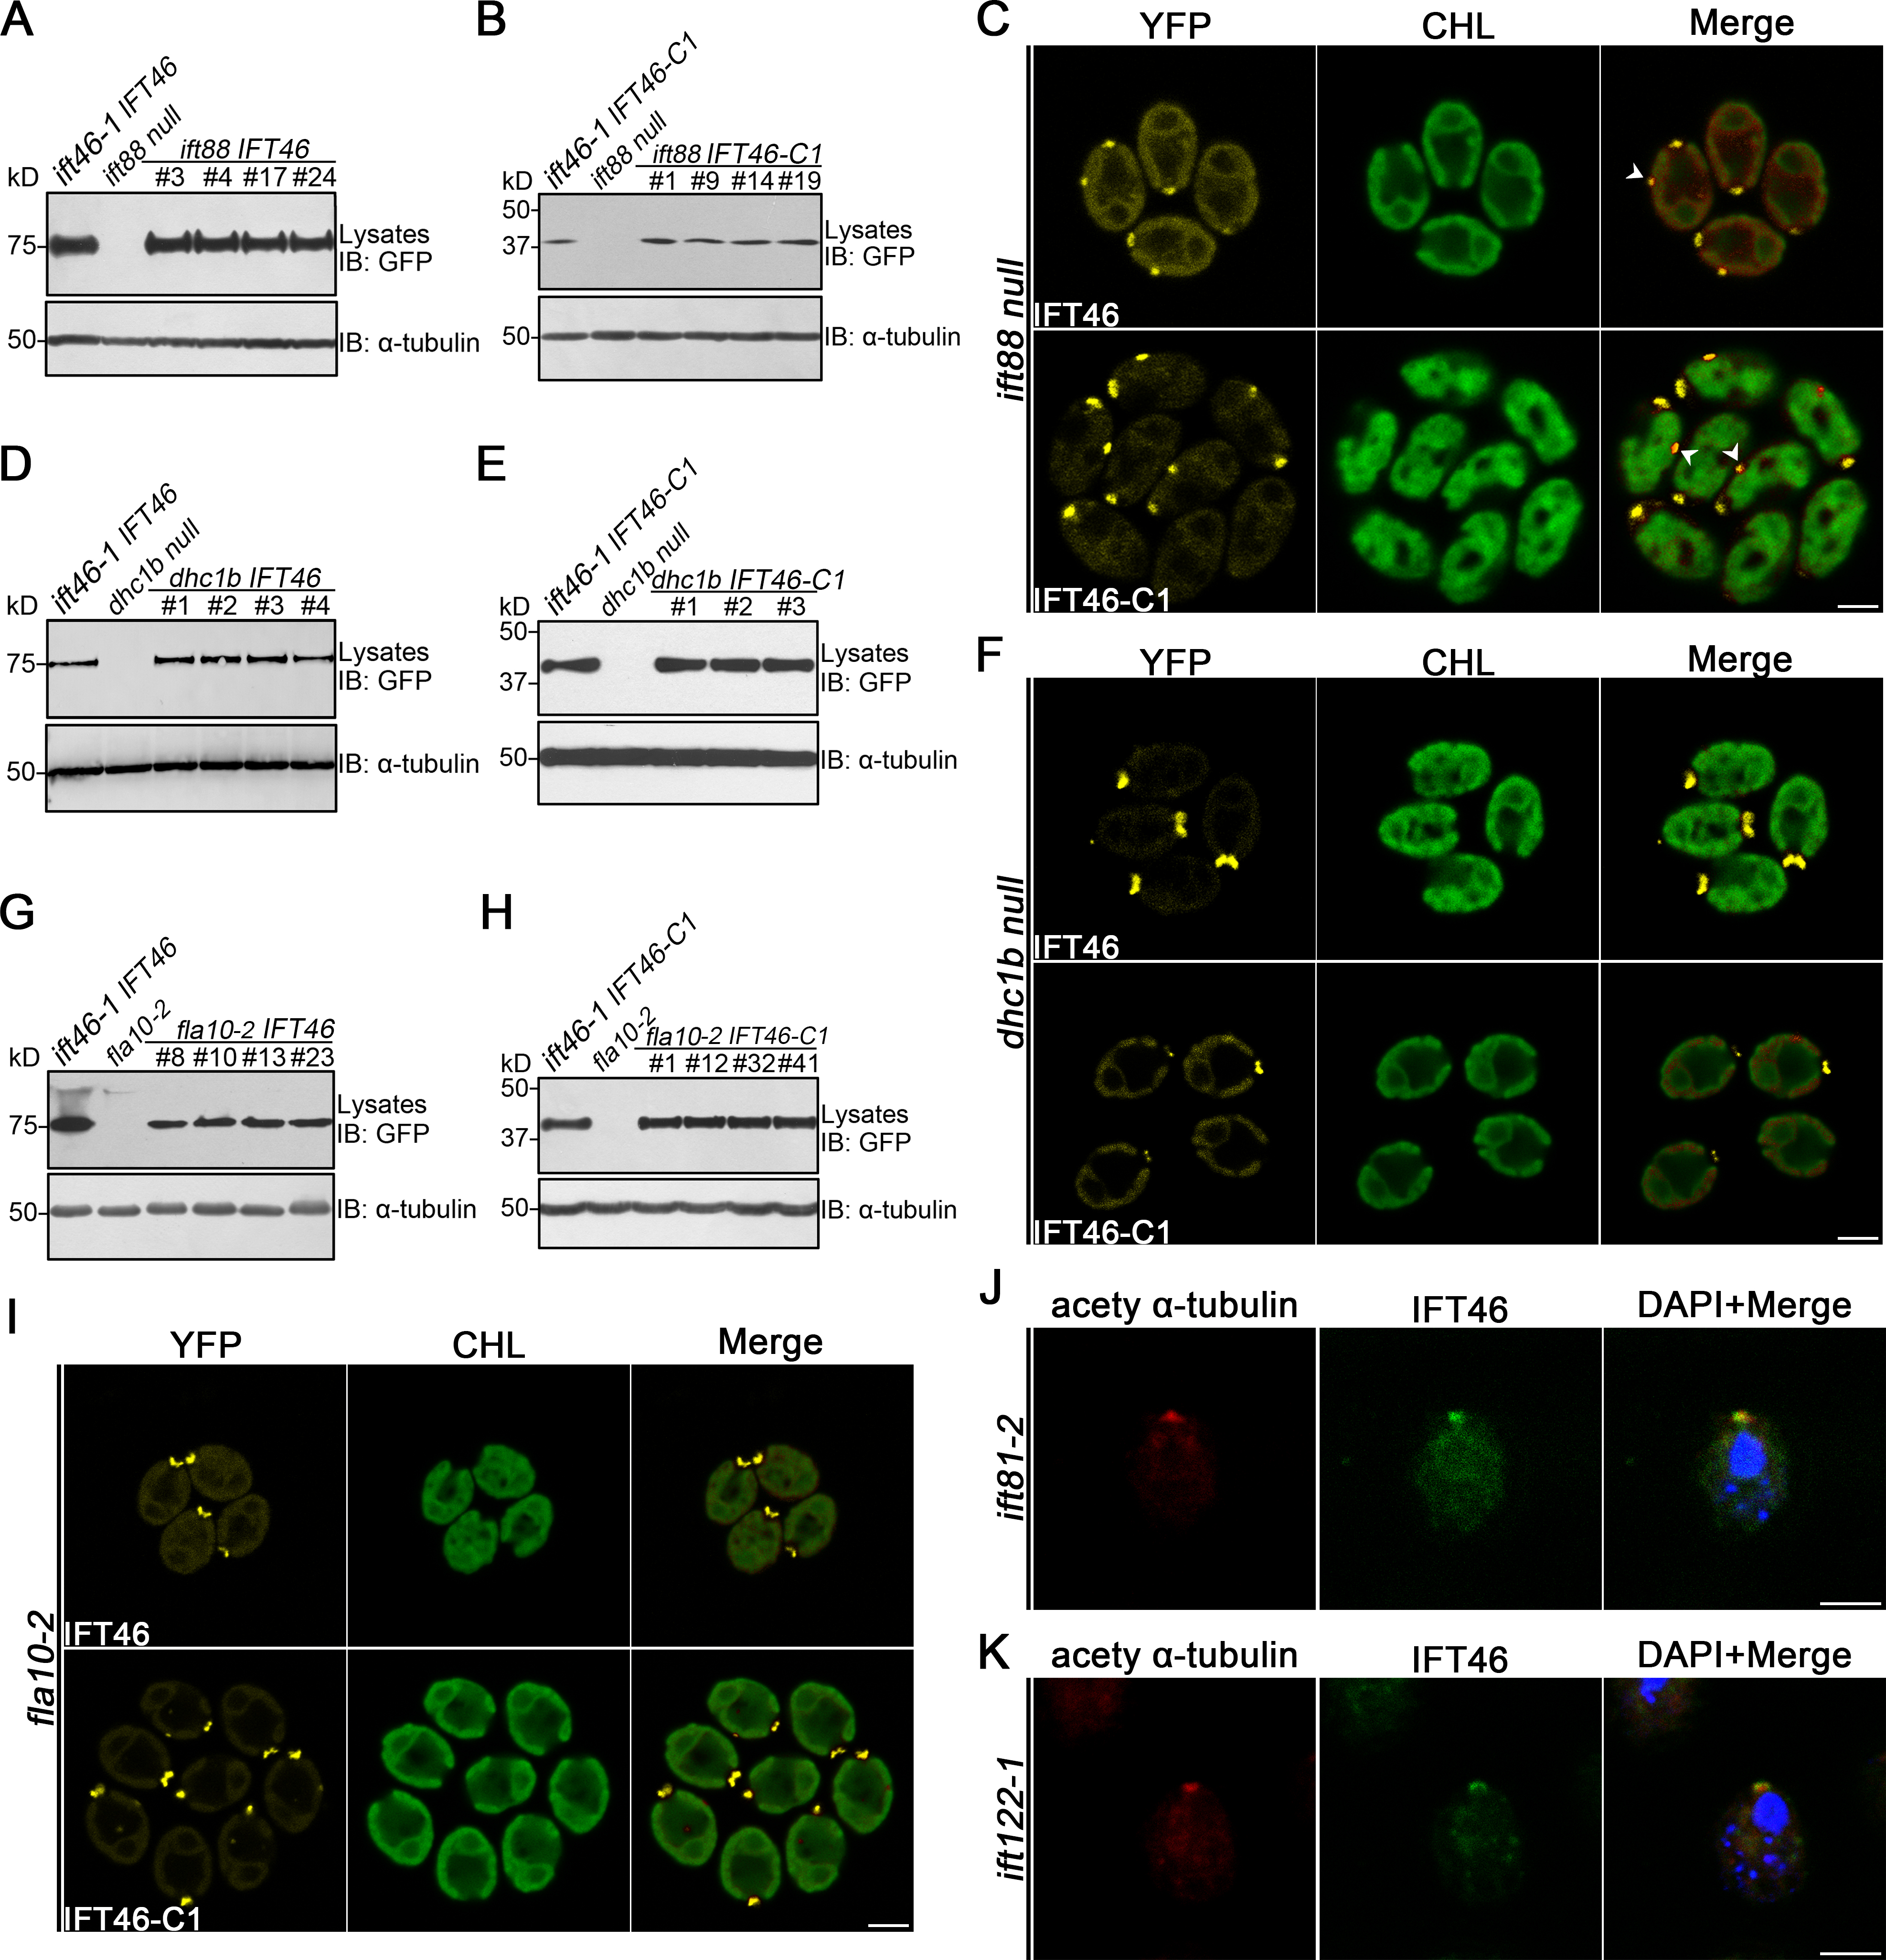
\includegraphics[width=\textwidth]{fig5-3.jpg}
%生成中英双语标题
{\setstretch{1.45}
\bicaption[fig:5.3]{图}{IFT46\ 的基体定位不依赖\ IFT122, IFT88, IFT81, FLA10\ 或\ DHC1b。(A,B,D,E,G,H)全细胞裂解物免疫印迹分析。(C,F,I)藻株的共聚焦成像分析。白色箭头标示眼点。(J,K)藻株\ \textit{ift81-2}\ (J)和\ \textit{ift122-1}\ (K)的免疫荧光成像。
\textcolor{red}{红色}为乙酰化\ $\upalpha$-tubulin,\textcolor{green}{绿色}为\ IFT46,\textcolor{blue}{蓝色}为标示细胞核的\ DAPI。 在\ A、B、D、E、G\ 和\ H\ 中,每个泳道的上样量为\ \SI{5}{\ug}。CHL\ 代表叶绿色。IB\ 代表免疫印迹。在\ C、F、I、J\ 和\ K\ 中,标尺代表\ \SI{5}{\um}.}{Figure}{The basal body localization of IFT46 is independent of IFT122, IFT88, IFT81, FLA10 or DHC1b. (A, B, D, E, G, H) Western blots of whole-cell lysates of indicated strains. (C, F, I) Confocal imaging of indicated strains. White arrows mark the eyespots. (J, K) Immunofluorescence microscopy of \textit{ift81-2} (J) and ift122-1 (K) using anti-acetylated $\upalpha$-tubulin antibody (red), anti-IFT46 antibody (green) and DAPI (blue). In A, B, D, E, G, and H, five micrograms of protein were loaded into each lane. IB means immunoblot. In C, F, I, J, and K, scale bars represent 5 $\upmu$m. CHL means chlorophyll.}
\par}
%结束图片浮动体环境
\end{figure}

\subsection{IFT46\ 的基体定位不依赖\ IFT122、IFT88、IFT81、FLA10\ 或\ DHC1b}
根据已发表的结果,我们知道\ IFT46\ 至少与\ ODA16、IFT88、IFT81、IFT74、IFT70\ 和\ IFT52\ 存在相互作用\
\citep{Lucker2005,Lucker2010,Taschner2014,Taschner2011,Fan2010}。我们的问题是\ IFT46\ 的基体定位是否依赖其他\ IFT\ 组分。为解决这一问题,我们拟在\ IFT\ 相关的缺失突变体中表达\ IFT46::YFP\ 或\ IFT46-C1::YFP。 如果\ IFT46\ 的基体定位依赖某个组分,那么\ IFT46::YFP\ 或\ IFT46-C1::YFP\ 将无法继续定位在基体。

据此,我们在\ \textit{ift88}、\textit{fla10-2}\ 和\ \textit{dhc1b}\ 中表达了\ IFT46::YFP\ 或\ IFT46-C1::YFP
(图\ \ref{fig:5.3}A,B,D,E,G,H)。 这些藻株分别是\ IFT88、FLA10\ 和\ DHC1b\ 的缺失突变体。使用抗\ GFP\ 的抗体通过免疫印迹我们筛选到了阳性克隆(图
\ref{fig:5.3}A,B,D,E,G,H)。同时我们也通过免疫荧光观察了\ IFT46\ 在\ \textit{ift81-2}\ 和\ \textit{ift122-1}\ 中的亚细胞定位(图\ \ref{fig:5.3}J,K)。观察结果显示,IFT46::YFP\ 或\ IFT46-C1::YFP\ 仍然定位在\
\textit{ift88}、\textit{fla10-2}\ 或\ \textit{dhc1b}\ 的基体(图\ \ref{fig:5.3}C,F,I)。这表明\ IFT46\ 的基体定位不依赖\ IFT88、FLA10\ 或\ DHC1b。 在\ \textit{ift81-2}\ 或\ \textit{ift122-1} 中,IFT46\ 与乙酰化\ $\upalpha$\ 微管蛋白共定位,后者主要定位在突变体的基体和短小鞭毛中(图\ \ref{fig:5.3}J,K)。这些结果意味着\ IFT46\ 的基体定位在\ \textit{ift81-2}\ 或\
\textit{ift122-1}\ 中并未受到影响,其基体定位也不依赖\ IFT81\ 或\ IFT122。

\subsection{IFT46\ 的基体定位依赖\ IFT52}
%开始图片浮动体环境,其中!表示取消严谨限制,h表示在此处插入,t表示在本页或下一页顶部插入
\begin{figure}[h!tbp]
%居中对齐
\centering
%设置图片搜索路径,每个路径用{}括起来
\graphicspath{{figures/}}
%插入图片并设置图片宽度为文本宽度减10mm
\includegraphics[width=\textwidth]{fig5-4.jpg}
%生成中英双语标题
{\setstretch{1.55}
\bicaption[fig:5.4]{图}{IFT46\ 的基体定位依赖\ IFT52。(A) \textit{bld1}, CC-125\ 和
\textit{bld1} \textit{IFT46::YFP}\ 全细胞裂解物免疫印迹分析。IB\ 代表免疫印迹。(B) \textit{ift46-1} \textit{IFT46-C1::YFP}, \textit{bld1}\ 和\ \textit{bld1} \textit{IFT46-C1::YFP}\ 全细胞裂解物免疫印迹分析。IB\ 代表免疫印迹。(C)表达\ IFT46::YFP\ 或\ IFT46-C1::YFP\ 的\ \textit{bld1}\ 藻株的共聚焦成像分析。(D)\textit{bld1} \textit{IFT52::3HA}, \textit{bld1}\ 和\ \textit{bld1} \textit{IFT46::YFP IFT52::3HA}\ 全细胞裂解物免疫印迹分析。IB\ 代表免疫印迹。(E)\textit{bld1} \textit{IFT52::3HA}, \textit{bld1}\ 和\ \textit{bld1} \textit{IFT46-C1::YFP IFT52::3HA}\ 全细胞裂解物免疫印迹分析。IB\ 代表免疫印迹。(F)表达\ IFT46::YFP IFT52::3HA\ 或\ IFT46-C1::YFP IFT52::3HA\ 的\ \textit{bld1}\ 藻株的共聚焦成像分析。在\ C\ 和\ F\ 中标尺代表\ \SI{5}{\um}。}{Figure}{The basal body localization of IFT46 depends on IFT52. (A) Western blots of whole-cell lysates of \textit{bld1}, CC-125, and \textit{bld1} \textit{IFT46::YFP} probed with the anti-GFP antibody and anti-$\upalpha$-tubulin antibody. IB: immunoblot. (B) Western blots of whole-cell lysates of \textit{ift46-1} \textit{IFT46-C1::YFP}, \textit{bld1}, and \textit{bld1} \textit{IFT46-C1::YFP} probed with the indicated antibodies. IB: immunoblot. (C) Confocal imaging of \textit{bld1} expressing IFT46::YFP or IFT46-C1::YFP. (D) Western blots of whole-cell lysates of \textit{bld1} \textit{IFT52::3HA}, \textit{bld1}, and \textit{bld1} \textit{IFT46::YFP IFT52::3HA} probed with the indicated antibodies. IB: immunoblot. (E) Western blots of whole-cell lysates of \textit{bld1} \textit{IFT52::3HA}, \textit{bld1}, and \textit{bld1} \textit{IFT46-C1::YFP IFT52::3HA} probed with the indicated antibodies.IB: immunoblot. (F) Confocal imaging of \textit{bld1} expressing IFT46::YFP IFT52::3HA or IFT46-C1::YFP IFT52::3HA. In panel C and F, CHL means chlorophyll. Scale bars represent 5 $\upmu$m.}
\par}
%结束图片浮动体环境
\end{figure}

同样的,我们也在\ \textit{IFT52}\ 的缺失突变体\ \textit{bld1}\ 中表达了\ IFT46\ 或\ IFT46-C1 (图
\ref{fig:5.4}\allowbreak A,B)。对阳性克隆的观察结果显示\ IFT46\ 无法继续定位在\ \textit{bld1} \ 的基体周围(图
\ref{fig:5.4}C)。IFT52\ 处于\ IFT-B\ 复合物的核心,它与\ IFT-B1\ 和\ IFT-B2\ 的多个亚基之间均存在相互作用\
\citep{Taschner2016a,Lucker2005,Lucker2010,Taschner2011,Taschner2014,Katoh2016}。IFT52\ 的缺失可导致\ IFT-B\ 其他亚基的表达量下降\ \citep{Zhang2016,Deane2001,Collet1998,Brazelton2001}。然而,\ IFT46\ 或\ IFT46-C1\ 无法定位在\
\textit{bld1}\ 的基体不太可能是由表达量下降造成的。因为我们观察的阳性克隆是通过免疫印迹筛选到的高表达株(图\ \ref{fig:5.4}A,B)。总之,IFT46\ 的基体定位依赖\ IFT52。

如果\ IFT52\ 的缺失能够破坏\ IFT46\ 的基体定位,那么理论上重新表达\ IFT52\ 应该能够恢复\ IFT46\ 的基体定位。为了验证这一点,我们在\ \textit{bld1} \textit{IFT46::YFP}\ 或\ \textit{bld1} \textit{IFT46-C1::YFP} 中表达了\ IFT52::3HA (图
\ref{fig:5.4}C,D)。通过对筛选到的阳性克隆进行共聚焦成像,我们发现在\ \textit{bld1} \textit{IFT46::YFP IFT52::3HA}\ 或\ \textit{bld1} \textit{IFT46-C1::YFP IFT52::3HA}\ 中\ IFT46\ 又重新定位到了基体(图
\ref{fig:5.4}E)。这些结果进一步说明\ IFT46\ 的基体定位确实依赖\ IFT52。

然而,IFT46\ 的基体定位依赖\ IFT52\ 还是存在两种可能性。一种是二者的依赖是相互的,它们共同作用从而靶向基体。另一种是\ IFT52\ 作用在\ IFT46\ 的上游,IFT52\ 将\ IFT46\ 招募到基体。为了排除其中一种可能性,我们在\ \textit{IFT46}\ 的缺失突变体\
\textit{ift46-1}\ 中表达了\ IFT52::YFP(图
\ref{fig:5.5}A)。使用抗\ GFP\ 的抗体通过免疫印迹我们筛选到了阳性克隆。活细胞成像结果显示\ IFT52\ 能够正常定位到\
\textit{ift46-1}\ 的基体(图\ \ref{fig:5.5}B)。这表明\ IFT52\ 的基体定位并不依赖\ IFT46,IFT52\ 作用在\ IFT46\ 的上游。

%开始图片浮动体环境,其中!表示取消严谨限制,h表示在此处插入,t表示在本页或下一页顶部插入
\begin{figure}[ht]
%居中对齐
\centering
%设置图片搜索路径,每个路径用{}括起来
\graphicspath{{figures/}}
%插入图片并设置图片宽度为文本宽度减10mm
\includegraphics[width=\textwidth]{fig5-5.jpg}
%生成中英双语标题
{\setstretch{1.667}
\bicaption[fig:5.5]{图}{IFT52\ 的基体定位不依赖\ IFT46。(A)\textit{ift46-1} \textit{IFT46::YFP}, \textit{ift46-1}\ 和\ \textit{ift46-1} \textit{IFT52::YFP}\ 全细胞裂解物免疫印迹分析。每个泳道的上样量为\ \SI{5}{\ug}。IB\ 代表免疫印迹。(B)表达\ IFT52::YFP\ 的
\ \textit{ift46-1}\ 藻株的共聚焦成像分析。标尺代表\ \SI{5}{\um}。}{Figure}{The basal body localization of IFT52 does not depend on IFT46. (A) Western blots of whole-cell lysates of \textit{ift46-1} \textit{IFT46::YFP}, \textit{ift46-1}, and \textit{ift46-1} \textit{IFT52::YFP} probed with the indicated antibodies. Five micrograms of protein were loaded per lane. IB means immunoblot. (B) Confocal imaging of \textit{ift46-1} expressing IFT52::YFP. CHL means chlorophyll. Scale bar represents 5 $\upmu$m.}
\par}
%结束图片浮动体环境
\end{figure}

\subsection{IFT52\ 结合并招募\ IFT46\ 至基体}
IFT52\ 和\ IFT46\ 之间的相互作用已经在体外实验中得到验证\
\citep{Taschner2016a,Lucker2005,Lucker2010,Taschner2011,Taschner2014,Katoh2016}。这里我们发现\ IFT46\ 的基体定位依赖\ IFT52。因而我们猜测二者之间的相互作用可能介导了\ IFT46\ 的基体定位。使用抗\ HA\ 的抗体对\ \textit{bld1} \textit{IFT46-C1::YFP IFT52::3HA}\ 的全细胞裂解液进行免疫共沉淀分析,结果显示\ IFT46\ 或\ IFT46-C1\ 富集在沉淀物中(图
\ref{fig:5.6}A)。这表明\ IFT46-C1\ 与全长\ IFT46\ 一样也能够与\ IFT52\ 相互作用。

%开始图片浮动体环境,其中!表示取消严谨限制,h表示在此处插入,t表示在本页或下一页顶部插入
\begin{figure}[h!btp]
%居中对齐
\centering
%设置图片搜索路径,每个路径用{}括起来
\graphicspath{{figures/}}
%插入图片并设置图片宽度为文本宽度减10mm
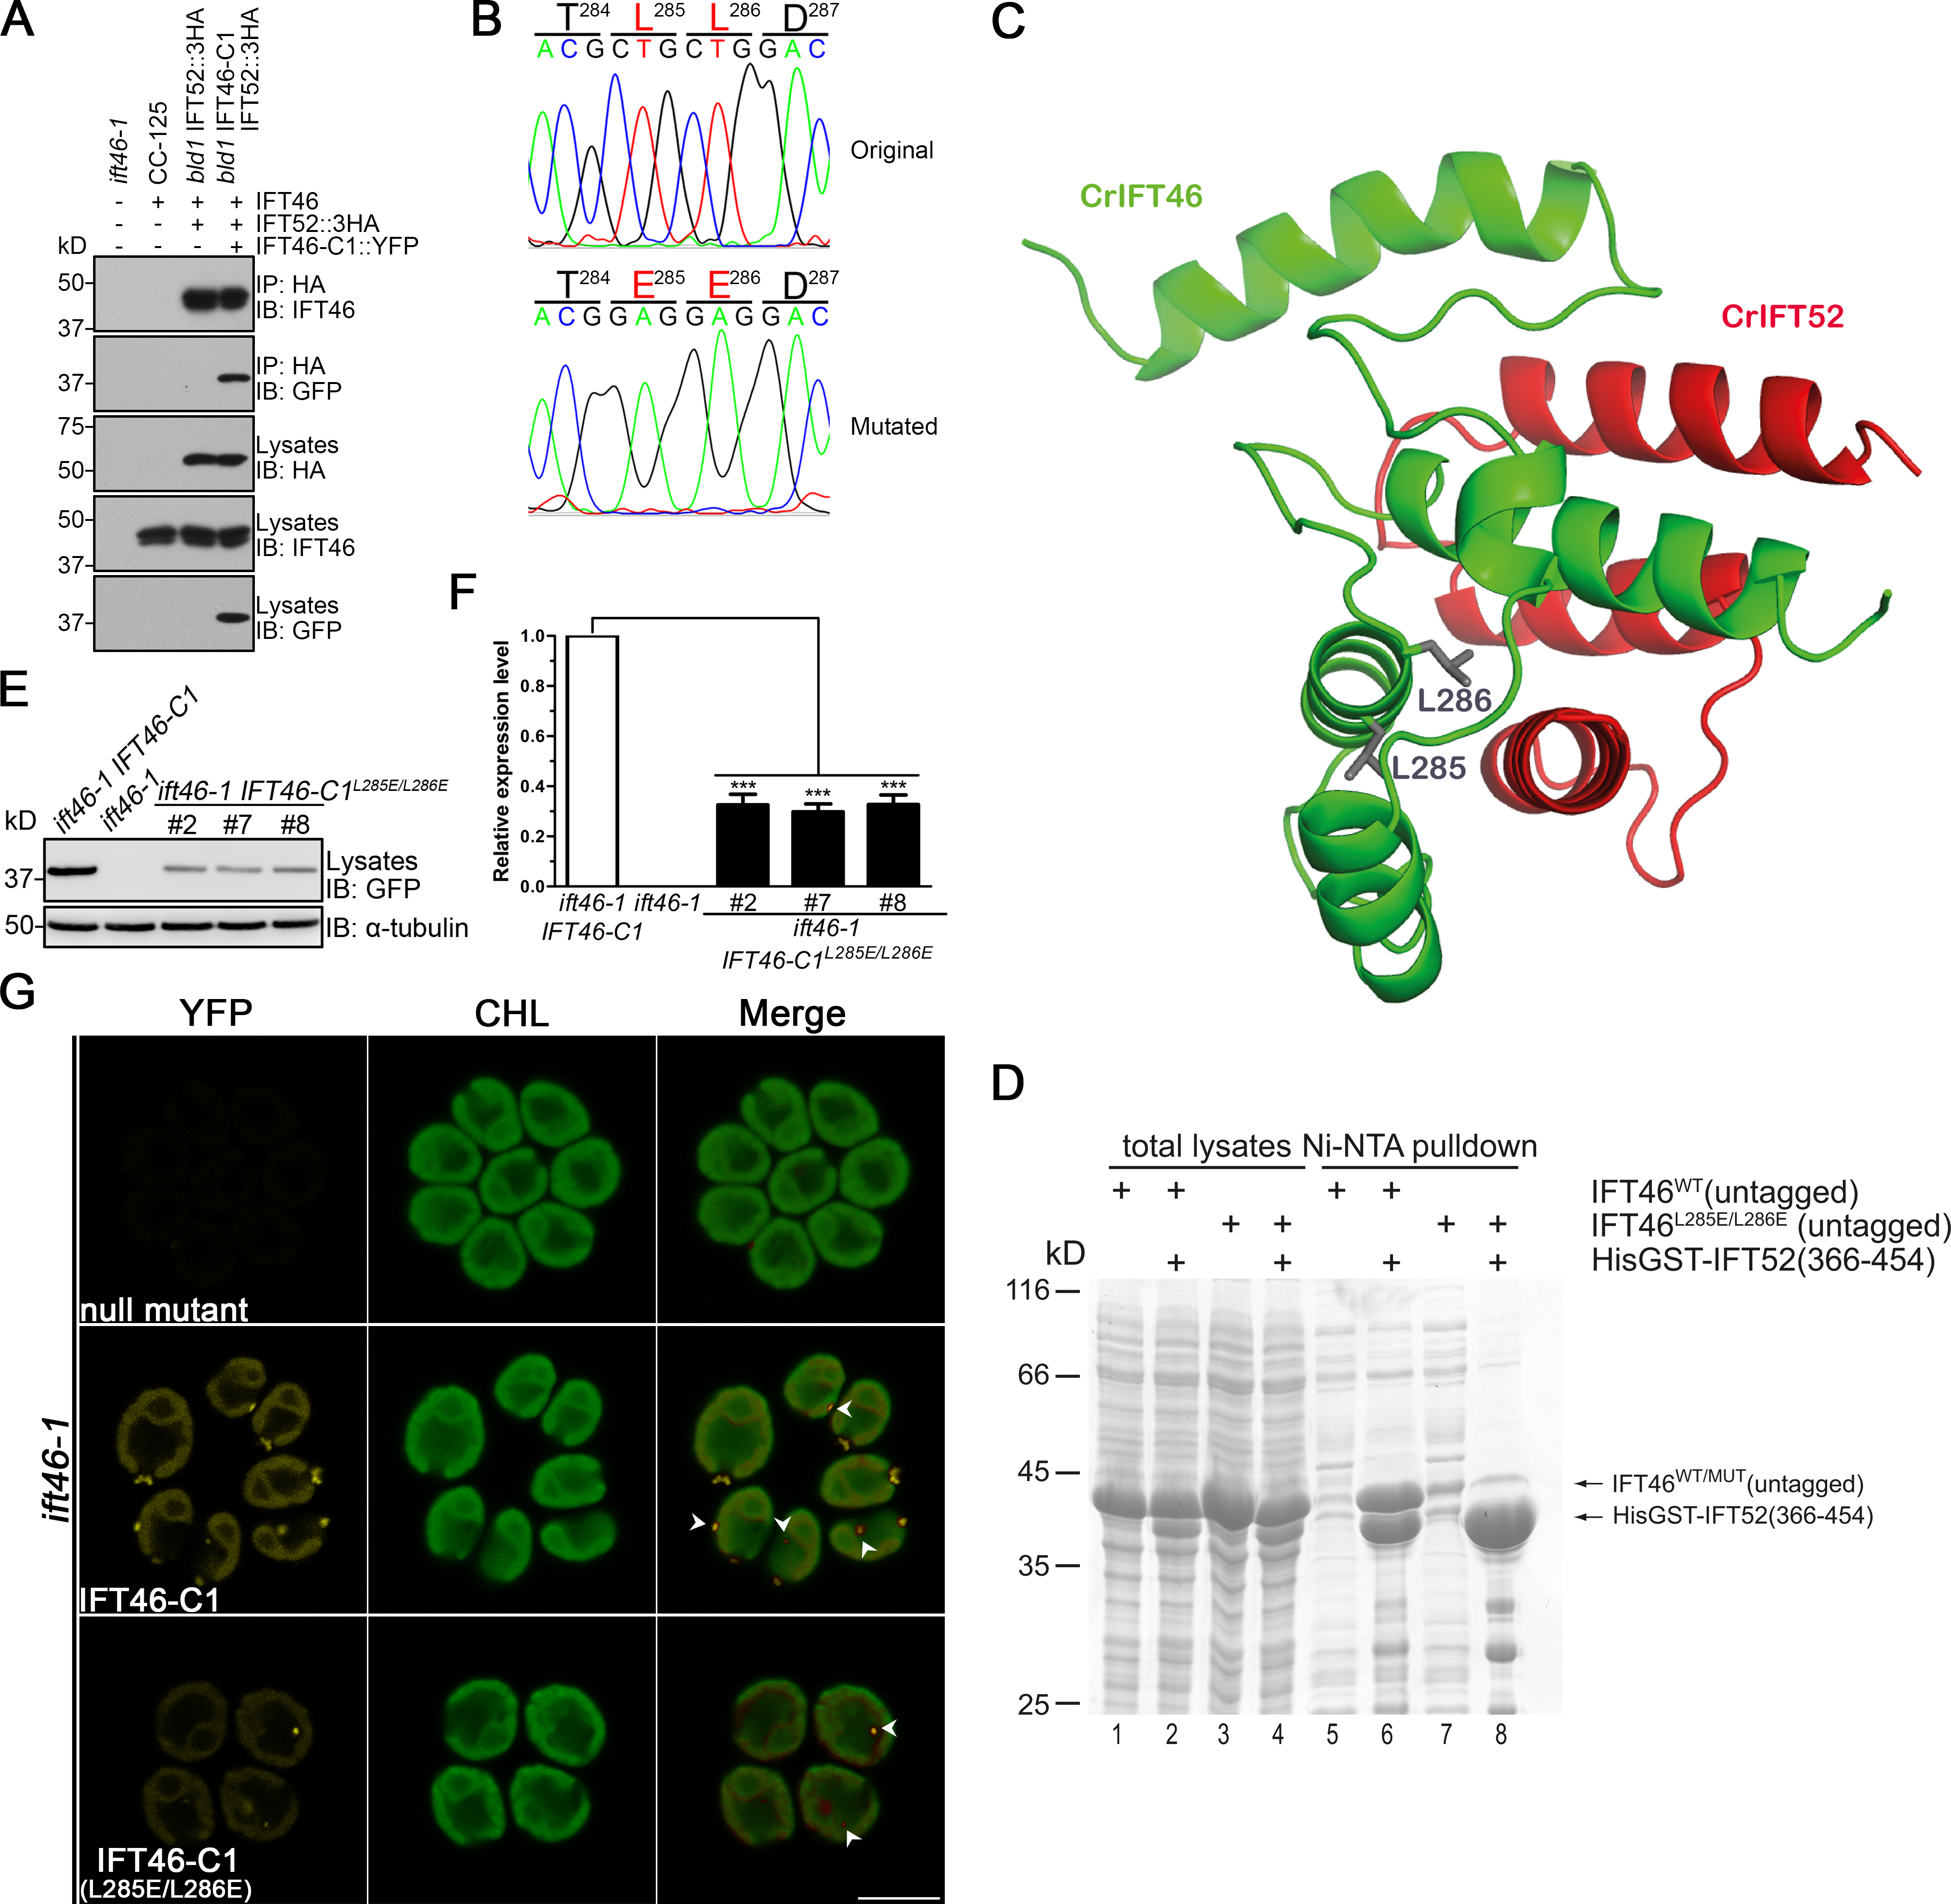
\includegraphics[width=\textwidth]{fig5-6.jpg}
%生成中英双语标题
{\setstretch{1.4}
\bicaption[fig:5.6]{图}{IFT52\ 结合并招募\ IFT46\ 至基体。(A)\ 用抗\ HA\ 的抗体对\ CC-125, \textit{bld1} \textit{IFT52::3HA}\ 和\ \textit{bld1} \textit{IFT46-C1 IFT52::3HA}\ 全细胞裂解液进行免疫共沉淀分析。(B)\ IFT46\ 定点突变示意图。(C)\ 基于\ TtIFT52C/46C\ 模拟的\ CrIFT52C/46C\ 的晶体结构。(D)\ Pull-down\ 分析显示\ GST-IFT52C\ 与\ IFT46$^{WT}$\ 相互作用,但不与\ IFT46$^{L285E/L286E}$\ 相互作用。(E)\ 全细胞裂解物免疫印迹分析。(F)\ IFT46-C1$^{L285E/L286E}$\ 相对于\ IFT46-C1\ 表达量显著下降。(G)\ 藻株的共聚焦成像分析。白色箭头表示眼点。CHL\ 代表叶绿素。标尺代表\ \SI{10}{\um}。}{Figure}{IFT52 binds and recruits IFT46 to the basal body. (A) Anti-HA antibody was used to immunoprecipitate HA-tagged IFT52. (B) Schematic diagram of site-directed mutagenesis of \textit{IFT46} gene. (C) The crystal structure of CrIFT52C/46C modeled based on TtIFT52C/46C. The two residues for mutagenesis were highlighted as grey sticks. (D) Pull-down of His-tagged GST-IFT52(366-454) with untagged IFT46$^{WT}$ or IFT46$^{L285E/L286E}$. (E) Western blots of whole-cell lysates (\SI{3}{\ug} protein per lane) of indicated strains. (F) Relative expression level of IFT46-C1$^{L285E/L286E}$ compared to the expression level of IFT46-C1. (G) Confocal imaging of indicated strains. White arrows, eyespots; CHL, chlorophyll; Scale bar, 10 $\upmu$m.}
\par}
%结束图片浮动体环境
\end{figure}

为了进一步测试\ IFT52\ 与\ IFT46\ 之间的相互作用是否是\ IFT46\ 基体定位所必须的,我们将\ IFT46-C1\ 上的两个关键的疏水亮氨酸突变为谷氨酸(图\ \ref{fig:5.6}B)。这两个亮氨酸在进化上高度保守(图\ \ref{fig:4.10})。从\ CrIFT52C/46C\ 的晶体结构(依据\ TtIFT52C/46C\ 的晶体结构模拟产生)上可以看到二者位于\ IFT52C\ 和\ IFT46C\ 的结合界面上
(图\ \ref{fig:5.6}C)\citep{Taschner2014}。将\ IFT52C\ 与突变后的\ IFT46\ 共表达在大肠杆菌中,结果显示\ IFT46$^{L285E/L286E}$\ 无法继续结合\ IFT52C(图\ \ref{fig:5.6}D)。与野生型\ IFT46-C1\ 相比,表达在\ \textit{ift46-1}\ 中的\ IFT46-C1$^{L285E/L286E}$\ 的表达量下降至约\ 32\%(
图\ \ref{fig:5.6}E,F)。由于\ IFT46$^{L285E/L286E}$\ 无法与\ IFT52\ 相互作用形成复合物,这种表达量的下降很可能是由于游离的\ IFT46-C1$^{L285E/L286E}$\ 被降解造成的。如图\ \ref{fig:5.6}G\ 所示,IFT46-C1\ 中第\ 285\ 和\ 286\ 号残基的突变破坏了其基体定位。由于\ IFT46-C1\ 和\ BBTS3\ 在表达量下降至约\ 30\%\ 时仍然能够定位到基体(图\ \ref{fig:4.9},\ref{fig:4.8}),IFT46-C1$^{L285E/L286E}$\ 的基体定位消失应该不是由于表达量下降造成的。这些结果表明\ IFT46-C1\ 与\ IFT52\ 之间的相互作用对\ IFT46\ 的基体定位至关重要。IFT52\ 结合并招募\ IFT46\ 至基体。

\subsection{构建表达\ IFT52C::YFP::NLS\ 的载体}
%开始图片浮动体环境,其中!表示取消严谨限制,h表示在此处插入,t表示在本页或下一页顶部插入
\begin{figure}[ht]
%居中对齐
\centering
%设置图片搜索路径,每个路径用{}括起来
\graphicspath{{figures/}}
%插入图片并设置图片宽度为文本宽度减10mm
\includegraphics[width=\textwidth]{fig5-X.jpg}
%生成中英双语标题
{\setstretch{1.667}
\bicaption[fig:5.X]{图}{构建表达\ IFT52C::YFP::NLS\ 的载体\ pHK473。(A)\ 菌液\ PCR\ 筛选阳性克隆后的电泳结果。(B)\ 对图\ A\ 中的三个阳性克隆进行酶切验证。}{Figure}{The construction of pHK473 which can express IFT52C::YFP::NLS. (A) agarose gel electrophoresis of bacteria colony polymerase chain reaction product to screen positive clones. (B) Agarose gel electrophoresis of restriction enzyme digestion product of three representative positive clones.}
\par}
%结束图片浮动体环境
\end{figure}

IFT46-C1\ 是\ IFT46\ 的基体和纤毛定位序列。IFT52\ 结合并招募\ IFT46\ 至基体。根据已有的报道我们还知道衣藻中部分\ IFT46\ 与胞质囊泡关联并被转运到基体\ \citep{Wood2014}。然而,关于\ IFT46\ 基体定位的分子机制仍然存在两种可能性。一种是\ IFT52\ 和\ IFT46\ 独立定位基体并在基体中发生相互作用形成复合物。另一种是新合成的\ IFT46\ 和\ IFT52\ 在胞质中预组装成亚复合物并定位到基体。这两种途径的关键差别在于\ IFT46\ 和\ IFT52\ 发生相互作用形成复合物的位置。在第一种途径中,二者在基体发生相互作用。而在第二种途径中二者在胞质或\ TGN\ 中形成亚复合物。为了排除其中一种可能性,我们拟将\ IFT52C\ 异位表达在衣藻细胞核并检查\ IFT46\ 是否跟随\ IFT52C\ 富集在细胞核。

为了构建表达\ IFT52C::YFP::NLS\ 的\ pHK473,我们以\ pHK470\ 为模板,利用引物\ IFT52C-F\ 和\ IFT52C-R\ 进行扩增,扩增产物经纯化后利用\ In-Fusion\ 方法重组克隆。随机挑选二十四个单克隆进行进行菌液\ PCR\ 检测,电泳结果显示其中十七个克隆可扩增出目的条带
(图\ \ref{fig:5.X}A)。 从这十七个疑似阳性克隆中选择三个扩大培养,抽提质粒进行酶切验证。电泳结果显示\ \#1\ 号和\ \#4\ 号克隆为阳性(图\ \ref{fig:5.X}B)。选定酶切大小正确的克隆进行测序验证,没有发生错义突变的\ \#4\ 号克隆用于后续实验。

\subsection{融合\ NLS\ 标签的\ IFT52C\ 可将\ IFT46\ 招募到细胞核}
%开始图片浮动体环境,其中!表示取消严谨限制,h表示在此处插入,t表示在本页或下一页顶部插入
\begin{figure}[h!tbp]
%居中对齐
\centering
%设置图片搜索路径,每个路径用{}括起来
\graphicspath{{figures/}}
%插入图片并设置图片宽度为文本宽度减10mm
\includegraphics[width=\textwidth]{fig5-7.jpg}
%生成中英双语标题
{\setstretch{1.52}
\bicaption[fig:5.7]{图}{带\ NLS\ 标签的\ IFT52C\ 将\ IFT46\ 招募至细胞核。(A)\ 全细胞裂解物免疫印迹分析。(B)\ 表达\ YFP, YFP::NLS\ 和\ IFT52C::YFP::NLS\ 的\ CC-125\ 藻株的共聚焦成像分析。(C)\ CC-125, CC-125 \textit{YFP}, CC-125 \textit{YFP::NLS}, \textit{bld1} \textit{IFT52::YFP}\ 和\ CC-125 \textit{IFT52C::YFP::NLS}\ 核裂解物免疫印迹分析。(D)\ 藻株\ CC-125 \textit{YFP::NLS}\ 和\ CC-125 \textit{IFT52C::YFP::NLS}\ 免疫荧光成像。\textcolor{red}{红色}为\ YFP::NLS\ 或\ IFT52C::YFP::NLS,\textcolor{green}{绿色}为\ IFT46,\textcolor{blue}{蓝色}为标示细胞核的\ DAPI。(E)\ 使用抗\ GFP\  的抗体针对带\ YFP\ 标签的\ IFT52C::YFP::NLS\ 对\ CC-125 \textit{IFT52C::YFP::NLS}\ 细胞核裂解液进行免疫共沉淀分析。沉淀产物用图示抗体进行检测。}{Figure}{NLS-tagged IFT52C recruits IFT46 to nuclei. (A) Western blots of whole-cell lysates (\SI{5}{\ug} protein per lane) of indicated strains. (B) Live cell imaging of CC-125 and CC-125 expressing YFP, YFP::NLS and IFT52C::YFP::NLS. CHL, chlorophyll. (C) Western blots of nuclear lysates (\SI{2}{\ug} protein per lane) of indicated strains. (D) Immunofluorescence microscopy of CC-125 \textit{YFP::NLS} and CC-125 \textit{IFT52C::YFP::NLS} using anti-GFP antibody (red), anti-IFT46 antibody (green) and 4, 6-diamidino-2-phenylindole (DAPI, blue). (E) Anti-GFP antibody was used to immunoprecipiate IFT52C::YFP::NLS from the nuclei of CC-125 \textit{IFT52C::YFP::NLS}. mIgG, IgG; IB, immunoblot; Scale bars, \SI{5}{\um}.}
\par}
%结束图片浮动体环境
\end{figure}

在植物、动物和病毒中存在多种核定位信号\ \citep{Lange2007,Rasala2014,Kropat2005,Kalderon1984}。 然而关于核定位信号在衣藻中的报道并不多\ \citep{Rasala2014,Lauersen2015}。本实验室前期的工作表明\ 4xSV40 NLS\ 能够有效的将\ YFP\ 带至衣藻细胞核(Wan et al., unpublished data)。为简便起见,后文所称\ NLS\ 均指的是\ 4xSV40 NLS。根据已有报道,IFT52\ 通过其\ C\ 端与\ IFT46\ 相互作用\
\citep{Taschner2016a,Lucker2005,Lucker2010,Taschner2011,Taschner2014,Katoh2016}。此外,在\ MDCK\ 细胞中过表达\ MmIFT52C\ 对初级纤毛的形成具有极强的显性负效应\ \citep{Taschner2014}。这可能是由其他\ IFT-B\ 蛋白的错误定位导致的\
\citep{Taschner2014}。以上事实表明将\ NLS\ 融合在\ IFT52C\ 上来研究\ IFT\ 蛋白的定位非常合适。

在野生型\ CC-125\ 细胞中,我们使用抗\ GFP\ 的抗体通过免疫印迹筛选出表达\ IFT52C::YFP::NLS\ 的阳性克隆(图\ \ref{fig:5.7}A)。通过共聚焦显微成像我们发现\ IFT52C::YFP::NLS\ 能够有效定位到衣藻细胞核(图\ \ref{fig:5.7}B)。对\ CC-125 \textit{IFT52C::YFP::NLS}\ 的细胞核的裂解液进行免疫印迹分析也证实\ IFT52C::YFP::NLS\ 确实成功在核内表达
(图\ \ref{fig:5.7}C)。与此同时,我们在\ CC-125 \textit{IFT52C::YFP::NLS}\ 的细胞核中也检测到了\ IFT46 (图\ \ref{fig:5.7}C)。免疫荧光实验的结果显示\ IFT46\ 除定位在基体和鞭毛外,在基体下方还与\ DAPI\ 共定位(图\ \ref{fig:5.7}D)。这表明\ IFT46\ 跟随\ IFT52C\ 进入了细胞核。使用抗\ GFP\ 的抗体对\ CC-125 \textit{IFT52C::YFP::NLS}\ 的核裂解液进行免疫共沉淀,结果显示\ IFT52C\ 与\ IFT46\ 均富集在沉淀物中(图\ \ref{fig:5.7}E)。这些数据表明\ IFT46\ 能够被融合了\ NLS\ 标签的\ IFT52C\ 招募到细胞核。这意味着二者在细胞质中已经预组装成亚复合物。

\section{讨论}
%开始图片浮动体环境,其中!表示取消严谨限制,h表示在此处插入,t表示在本页或下一页顶部插入
\begin{figure}[htbp]
%居中对齐
\centering
%设置图片搜索路径,每个路径用{}括起来
\graphicspath{{figures/}}
%插入图片并设置图片宽度为文本宽度减10mm
\includegraphics[width=\textwidth-80mm]{fig5-8.jpg}
%生成中英双语标题
{\setstretch{1.667}
\bicaption[fig:5.8]{图}{IFT46\ 基体定位的模型。核糖体上合成的\ IFT46\ 和\ IFT52\ 在胞质或高尔基体上预组装成亚复合物并经过囊泡或非囊泡介导的途径定位到基体。TGN\ 为反式高尔基体网络,BB\ 为基体。}{Figure}{Model for basal body localization of IFT46. Preassembled IFT52/46 subcomplex is targeted to basal body region through the vesicle-mediated or non-vesicle-mediated ways. TGN, trans-Golgi network; BB, basal body.}
\par}
%结束图片浮动体环境
\end{figure}

IFT46\ 的\ C\ 端是\ IFT46\ 的基体和纤毛定位序列\ \citep{Lv2017}。IFT52\ 结合并招募\ IFT46\ 至基体\ \citep{Lv2017}。同时\ IFT46\ 能够被含\ NLS\ 标签的\ IFT52C\ 招募到细胞核\ \citep{Lv2017}。这表明\ IFT46\ 和\ IFT52\ 是在胞质或\ TGN\ 中预组装而非在基体中才组装\ \citep{Lv2017}。在衣藻鞭毛再生过程中,IFT46\ 出现在来自\ TGN\ 的囊泡上\ \citep{Wood2014}。因而有可能\ IFT46\ 和\ IFT52\ 是在\ TGN\ 中预组装并通过囊泡介导的途径定位到基体(图\ \ref{fig:5.8})。然而,在\ IFT\ 蛋白中仅\ IFT20\ 曾被观察到定位在高尔基体,大部分\ IFT\ 蛋白均与膜没有关联\
\citep{Richey2012,Follit2006}。 因此我们无法排除这样一种可能性,即预组装的\ IFT46\ 和\ IFT52\ 通过非囊泡介导的途径定位到基体(图\ \ref{fig:5.8})。

与\ Lucker\ 和\ Richey\ 等人提出的关于\ IFT\ 复合物\ B\ 的组装模型相比,三者均认为\ IFT\ 复合物\ B\ 中的亚基预组装成亚复合物,这些亚复合物再组装成完整的复合物\ B\ \citep{Lucker2010,Richey2012,Lv2017}。 不同之处在于我们提供了有力的证据显示\ IFT52\ 作用在\ IFT46\ 的上游,发挥类似“种子”的作用\ \citep{Lv2017}。除了能够结合并招募\ IFT46,我们认为\ IFT52\ 很可能还招募了其他亚基。然而受限于相应的抗体和突变体,这种假设需要通过其他途径进行验证。此外,三个模型中关于复合物组装的位置有差异。Lucker\ 等人的模型未明确指出组装发生的地点\ \citep{Lucker2010}。这可能是由于他们的大部分结果均通过生化方法获得,缺少体内实验的验证。Richey\ 等人的模型则认为\ IFT\ 复合物\ B\ 的核心复合物可能在基体近端组装然后转移到过渡纤维\ \citep{Richey2012}。这种转变过程需要\ IFT88\ 和\ IFT\ 复合物\ B\ 外周亚基的参与\ \citep{Richey2012}。这一模型虽然信息完善,但大多属于猜测,可靠性有待进一步证实。根据我们的实验结果,我们认为\ IFT52\ 和\ IFT46\ 在胞质中预先组装成亚复合物然后再定位到基体(图\ \ref{fig:5.8})。当然,这里还有很多问题有待解决。比如还有哪些亚基参与了预组装,亚复合物定位到基体的什么部位等。一种可行的研究策略是异位表达\ IFT52,然后通过亲和纯化分离特定细胞器并通过质谱鉴定哪些蛋白跟随\ IFT52\ 发生了转位。

前面我们发现\ IFT46-C1\ 是\ IFT46\ 的基体定位序列。这里我们检测到\ IFT46-C1\ 直接与\ IFT52\ 相互作用(图\ \ref{fig:5.6})。通过突变\ IFT46-C1\ 上的关键残基来破坏\ IFT46-C1\ 与\ IFT52\ 之间的相互作用可阻断\ IFT46-C1\ 的基体定位(图\ \ref{fig:5.6})。这表明\ IFT52\ 直接介导了\ IFT46\ 的基体定位。然而,IFT46\ 的相互作用对象仍然是一个\ IFT\ 蛋白,IFT52。 这使得\ IFT46-C1\ 有别于其他的经典定位序列\
\citep{Malicki2014,Bhogaraju2013,McIntyre2015,Dishinger2010,Berbari2008,Hurd2011,Santos2014}。 在接下来的工作中我们需要在\ IFT52\ 或其他上游\ IFT\ 蛋白中鉴定到\ IFT\ 蛋白通用的定位序列。

\section{小结}
通过在\ IFT\ 相关蛋白的缺失突变体中表达\ IFT46\ 或\ IFT46-C1,我们发现\ IFT46\ 的基体定位不依赖\ IFT122、IFT88、IFT81、FLA10\ 或\ DHC1b,但是依赖\ IFT52。同时\ IFT52\ 的基体定位并不依赖\ IFT46。 这说明\ IFT52\ 作用在\ IFT46\ 的上游。进一步研究发现\ IFT52\ 能够结合并招募\ IFT46\ 至基体。通过在细胞核中表达\ IFT52C,我们成功将\ IFT46\ 招募到细胞核。这些结果表明\ IFT46\ 和\ IFT52\ 在细胞质或\ TGN\ 中预组装成亚复合物然后定位到基体(图\ \ref{fig:5.8})。 
%调入第X章,不要加拓展名tex。最后版本中删除。
%input和include命令均能够调入子文档,但include会重启一页
%\include{chapterx}
%%%%%%%%%%%%%%%%%%%%%%%%%%%%%%%%%%%%%%%%%%%%%%%%%%%%%%%%%%%%%%%%%%%%%%%%%%%%%%%%%%%%%%%%%%%%%%%%%%%%%%%%
%开始后文区。
\backmatter
%调入总结,不要加拓展名tex
%input和include命令均能够调入子文档,但include会重启一页
\chapter{总\quad 结}
\renewcommand{\leftmark}{总\quad 结}

\Blindtext

\Blindtext

\Blindtext
%调入参考文献,不要加拓展名tex。
%input和include命令均能够调入子文档,但include会重启一页
%空行代表重启一个段落。
%如果这里采用chapter插入参考文献会产生两页空白,因为\bibliography{library1}命令又会重启一章
%\chapter{参考文献}
%如果使用article文类请使用\clearpage命令,该命令可以解决手动添加目录到目录中页码不一致的问题
\cleardoublepage
%如果使用了Hyperref宏包生成书签,还需要使用命令,否则书签中显示不正常
\phantomsection
\addcontentsline{toc}{chapter}{参考文献}
%直接在奇数页页眉中显示章标题会多处一些章标题内部编号,这里重新定义\leftmark,后续所有章节都要重新定义
\renewcommand{\leftmark}{参考文献}
%%%%%%%%%%%%%%%%%%%%%%%%%%%%%%%%%%%%%%%%%%%%%%%%%%%%%%%%%%%%%%%%%%%%%%%%%%%%%%%%%%%%%%%%%%%%%%%%%%%%%%%
%     可用的引文插入命令。这些命令有natbib宏包提供。了解更多请谷歌一下。
%     \cite{jon90} =) Jones et al. (1990)
%     \citet{jon90} =) Jones et al. (1990)
%     \citet[Chap.2]{jon90} =) Jones et al. (1990, Chap. 2)
%     \citet*{jon90} =) Jones, Baker, and Williams (1990)
%     \citep{jon90} =) (Jones et al., 1990)
%     \citep*{jon90} =) (Jones, Baker, and Williams, 1990)
%%%%%%%%%%%%%%%%%%%%%%%%%%%%%%%%%%%%%%%%%%%%%%%%%%%%%%%%%%%%%%%%%%%%%%%%%%%%%%%%%%%%%%%%%%%%%%%%%%%%%%%%
%缩小参考文献列表字号
\small
%调整条目从第二行开始的缩进
\setlength{\bibhang}{0pt}
%重定义文献条目编号。理论上默认的的应该就有,不知为何需要重写一遍才出来。
\makeatletter
\renewcommand\@biblabel[1]{[#1]}
\makeatother
%调入参考文献格式文档,不需要拓展名bst。doctor.bst文档放在主tex文档文件夹中。
\bibliographystyle{doctor}
%\bibliographystyle{google1}
%调入参考文献库文档,不需要拓展名bib。多个文献库名之间用逗号分开且没有空格。PHD.bib文档放在主tex文档文件夹中。
\bibliography{PHD}
%恢复后文字号
\normalsize
%调入附录A,不要加拓展名tex。
%input和include命令均能够调入子文档,但include会重启一页
%空行代表重启一个段落。
%开始插入附录
%\appendix
\chapter{附录A\quad 本研究所用仪器信息}\label{appen:A}
%直接在奇数页页眉中显示章标题会多处一些章标题内部编号,这里重新定义\leftmark,后续所有章节都要重新定义
\renewcommand{\leftmark}{附录A\quad 本研究所用仪器信息}
%将章节号计数器设置为1
\setcounter{chapter}{1}
%将插图序号计数器设置为1
\setcounter{figure}{0}
%将表格序号计数器设置为1
\setcounter{table}{0}
\renewcommand{\thechapter}{\Alph{chapter}}
%改变图表标题的编号形式(该命令有ccaption宏包提供)
\makeatletter
\@removefromreset{table}{chapter}
\renewcommand{\thetable}{\arabic{table}}
\@removefromreset{figure}{chapter}
\renewcommand{\thefigure}{\arabic{figure}}
\makeatother
%重定义图表标题形式(LaTeX中的计数器本身可以通过这种方式加前缀或后缀)
\renewcommand{\thetable}{\thechapter\arabic{table}}
\renewcommand{\thefigure}{\thechapter\arabic{figure}}
%利用左右盒子为长表添加标题。不推荐用这种方法,但是目前还没有找到能用的手段。
\makebox[\textwidth][c]{\small 表A1 本研究所用仪器信息。}
%这里必须空一行。

\makebox[\textwidth][c]{\small Table A1 List of instruments used in this study.}
%调整字号
\small
%插入表格但是最多有一种语言的标题。如果需要双语标题就留空然后在PDF中编辑。
\LTXtable{\textwidth}{appendagesAcode.tex}
%调整字号
\normalsize





%调入附录B,不要加拓展名tex。
%input和include命令均能够调入子文档,但include会重启一页
\chapter{附录B\quad 本研究所用试剂信息}
\renewcommand{\leftmark}{附录B\quad 本研究所用试剂信息}
\setcounter{chapter}{2}
\setcounter{figure}{0}
\setcounter{table}{0}

\blindtext

\blindtext

\blindtext
%调入附录C,不要加拓展名tex。附录C已经调试好,暂时不调入!!!
%input和include命令均能够调入子文档,但include会重启一页
%空行代表重启一个段落。
%开始插入附录
%\appendix
\chapter{附录C\quad 本研究所用培养基}\label{appen:C}
%直接在奇数页页眉中显示章标题会多处一些章标题内部编号,这里重新定义\leftmark,后续所有章节都要重新定义
\renewcommand{\leftmark}{附录C\quad 本研究所用培养基}
%将章节号计数器设置为3
\setcounter{chapter}{3}
%将插图序号计数器设置为1
\setcounter{figure}{0}
%将表格序号计数器设置为1
\setcounter{table}{0}

%开始表格浮动体环境,其中!表示取消严谨限制,h表示在此处插入,t表示在本页或下一页顶部插入
\begin{table}[htbp]
%调整字号
\small
%居中对齐
\centering
%生成中英双语标题
{\setstretch{1.667}
\bicaption[tab:tableC1]{表}{TAP\ 培养基配方。}{Table}{Formulation of the TAP medium.}
\par}
%开始绘制表格
\begin{tabular*}{\textwidth}[c]{@{\extracolsep{\fill}}lll}
%绘制一条水平线
\toprule
编号\ (Number) & 母液\ (Stock Solution) & 体积或质量\ (Volume or Mass)\\
\midrule
1 & 100xTris* & 10 mL\\
2 & 100xTAP salts** & 10 mL\\
3 & Phosphate salts** & 1 mL\\
4 & Trace metals** & 1 mL\\
5 & Glacial acetic acid & 1 mL\\
6 & Agar (for solid medium only) & 15 g\\
7 & ddH$_2$O & To 1 L\\
\bottomrule
\multicolumn{2}{l}{*Dissolve 24.2g Tris in 100 mL water.}\\
\multicolumn{2}{l}{**See below for detailed information.}
%结束绘制表格
\end{tabular*}
%结束表格浮动体环境
\end{table}

\vspace{35pt}

%开始表格浮动体环境,其中!表示取消严谨限制,h表示在此处插入,t表示在本页或下一页顶部插入
\begin{table}[htbp]
%调整字号
\small
%居中对齐
\centering
%生成中英双语标题
{\setstretch{1.667}
\bicaption[tab:tableC2]{表}{100x TAP salts\ 配方。}{Table}{Formulation of 100x TAP salts used for the TAP medium.}
\par}
%开始绘制表格
\begin{tabular*}{\textwidth}[c]{@{\extracolsep{\fill}}lll}
%绘制一条水平线
\toprule
编号\ (Number) & 试剂\ (Reagents) & 质量或体积\ (Mass or Volume)\\
\midrule
1 & NH$_4$Cl & 37.5 g\\
2 & MgSO$_4$$\cdot$7H$_2$O & 10 g\\
3 & CaCl$_2$$\cdot$H$_2$O & 5 g\\
4 & ddH$_2$O & To 1 L\\
\bottomrule
%结束绘制表格
\end{tabular*}
%结束表格浮动体环境
\end{table}

\vspace{35pt}

%开始表格浮动体环境,其中!表示取消严谨限制,h表示在此处插入,t表示在本页或下一页顶部插入
\begin{table}[htbp]
%调整字号
\small
%居中对齐
\centering
%生成中英双语标题
{\setstretch{1.667}
\bicaption[tab:tableC3]{表}{Phosphate salts\ 配方。}{Table}{Formulation of Phosphate salts used for the TAP medium.}
\par}
%开始绘制表格
\begin{tabular*}{\textwidth}[c]{@{\extracolsep{\fill}}lll}
%绘制一条水平线
\toprule
编号\ (Number) & 试剂\ (Reagents) & 质量或体积\ (Mass or Volume)\\
\midrule
1 & K$_2$HPO$_4$ & 54 g\\
2 & KH$_2$PO$_4$ & 27 g\\
3 & ddH$_2$O & To 500 mL\\
\bottomrule
%结束绘制表格
\end{tabular*}
%结束表格浮动体环境
\end{table}

%开始表格浮动体环境,其中!表示取消严谨限制,h表示在此处插入,t表示在本页或下一页顶部插入
\begin{table}[htbp]
%调整字号
\small
%居中对齐
\centering
%生成中英双语标题
{\setstretch{1.667}
\bicaption[tab:tableC4]{表}{Trace metals\ 配方*。}{Table}{Formulation of Trace metals used for the TAP medium.}
\par}
%开始绘制表格
\begin{tabular*}{\textwidth}[c]{@{\extracolsep{\fill}}llll}
%绘制一条水平线
\toprule
编号\ (Number) & 试剂\ (Reagents) & 质量\ (Mass)  & 去离子水体积\ (Volume of ddH$_2$O)\\
\midrule
1 & EDTA disodium salt   & 50 g  & 250 mL\\
2 & ZnSO$_4$$\cdot$7H$_2$O           &22 g   & 100 mL\\
3 & H$_3$BO$_3$                &11.4 g & 200 mL\\
4 & MnCl$_2$$\cdot$4H$_2$O           &5.06 g & 50 mL\\
5 & CoCl$_2$$\cdot$6H$_2$O           &1.61 g & 50 mL\\
6 & CuSO$_4$$\cdot$5H$_2$O           &1.57 g & 50 mL\\
7 & (NH$_4$)$_6$Mo$_7$O$_{24}$$\cdot$4H$_2$O    &1.1 g  & 50 mL\\
8 & FeSO$_4$$\cdot$7H$_2$O           &4.99 g & 50 mL\\
\bottomrule
%结束绘制表格
\end{tabular*}
%结束表格浮动体环境
\end{table}
*Dissolve each compound in the volume of water indicated. The EDTA disodium salt should be dissolved in boiling water, and the FeSO$_4$ should be prepared last to avoid oxidation. Mix all solutions except EDTA disodium salt. Bring this mixture to boil and add EDTA disodium salt solution. The mixture should turn green. When everything is dissolved, cool to \SI{70}{\degreeCelsius}. Keeping temperature at \SI{70}{\degreeCelsius}, adjust the pH to 6.7 with 50 mL KOH (20\%). Remember to standardize the pH meter with buffer at the same temperature. Do not use NaOH to adjust the pH value. Bring the final solution to 1 liter. It should be clear green initially. Stopper the flask with a cotton plug and let it stand for 1-2 weeks, shaking it once a day. The solution should eventually turn purple and leave a rust-brown precipitate, which can be removed by filtering through two layers of Whatman \#1 filter paper, repeating the filtration if necessary until the solution is clear. It can be stored refrigerated or frozen in convenient aliquots.

\vfill

%开始表格浮动体环境,其中!表示取消严谨限制,h表示在此处插入,t表示在本页或下一页顶部插入
\begin{table}[htbp]
%调整字号
\small
%居中对齐
\centering
%生成中英双语标题
{\setstretch{1.667}
\bicaption[tab:tableC5]{表}{MI\ 培养基配方*。}{Table}{Formulation of the MI medium.}
\par}
%开始绘制表格
\begin{tabular*}{\textwidth}[c]{@{\extracolsep{\fill}}lll}
%绘制一条水平线
\toprule
母液\ (Stock Solution) & 浓度\ (Concentration)     & 体积或质量\ (Volume or Mass)\\
\midrule
C$_6$H$_5$Na$_3$O$_7$$\cdot$2H$_2$O& 500 g/L  &1 mL       \\
 FeCl$_3$$\cdot$6H$_2$O             &10 g/L    &1 mL       \\
 CaCl$_2$$\cdot$2H$_2$O             & 53 g/L   &1 mL       \\
 MgSO$_4$$\cdot$7H$_2$O             & 300 g/L  &1 mL       \\
 NH$_4$NO$_3$                       & 450 g/L  &1 mL       \\
K$_2$HPO$_4$                       & 200 g/L  &0.5 mL     \\
 KH$_2$PO$_4$                       & 200 g/L  &0.5 mL     \\
 Trace elements                     & No       &1 mL       \\
 H$_3$BO$_3$                        & 1 g/L    &No         \\
 ZnSO$_4$$\cdot$7H$_2$O             & 1 g/L    &No         \\
 MnSO$_4$$\cdot$H$_2$O              & 0.3 g/L  &No         \\
 CoCl$_2$$\cdot$6H$_2$O             & 0.2 g/L  &No         \\
Na$_2$MoO$_4$$\cdot$2H$_2$O        & 0.2 g/L  &No         \\
CuSO$_4$$\cdot$5H$_2$O             & 0.04 g/L &No         \\
 Agar (for solid medium only)       & No       & 15 g      \\
 ddH$_2$O                           & No       & To 1 L    \\
\bottomrule
\multicolumn{3}{l}{*Adjust pH value to 6.9 before bring the final solution to 1 L.}
%结束绘制表格
\end{tabular*}
%结束表格浮动体环境
\end{table}


%开始表格浮动体环境,其中!表示取消严谨限制,h表示在此处插入,t表示在本页或下一页顶部插入
\begin{table}[htbp]
%调整字号
\small
%居中对齐
\centering
%生成中英双语标题
{\setstretch{1.667}
\bicaption[tab:tableC6]{表}{LB\ 培养基配方。}{Table}{Formulation of the LB medium.}
\par}
%开始绘制表格
\begin{tabular*}{\textwidth}[c]{@{\extracolsep{\fill}}lll}
%绘制一条水平线
\toprule
编号\ (Number) & 试剂\ (Reagents) & 质量或体积\ (Mass or Volume)\\
\midrule
1 & Tryptone                     & 10 g\\
2 & Yeast Extract                & 5 g\\
3 & NaCl                         & 10 g\\
4 & Agar (for solid medium only) & 15 g\\
5 & ddH$_2$O                     & To 1 L\\
\bottomrule
%结束绘制表格
\end{tabular*}
%结束表格浮动体环境
\end{table}

%开始表格浮动体环境,其中!表示取消严谨限制,h表示在此处插入,t表示在本页或下一页顶部插入
\begin{table}[htbp]
%调整字号
\small
%居中对齐
\centering
%生成中英双语标题
{\setstretch{1.667}
\bicaption[tab:tableCX]{表}{SOB\ 培养基配方。}{Table}{Formulation of the SOB medium.}
\par}
%开始绘制表格
\begin{tabular*}{\textwidth}[c]{@{\extracolsep{\fill}}lll}
%绘制一条水平线
\toprule
编号\ (Number) & 试剂\ (Reagents) & 质量或体积\ (Mass or Volume)\\
\midrule
1 & Tryptone                     & 10 g\\
2 & Yeast Extract                & 2.5 g\\
3 & NaCl                         & 0.25 g\\
4 & KCl                          & 0.093 g\\
5 & ddH$_2$O                     & To 500 mL\\
\bottomrule
%结束绘制表格
\end{tabular*}
%结束表格浮动体环境
\end{table}

%开始表格浮动体环境,其中!表示取消严谨限制,h表示在此处插入,t表示在本页或下一页顶部插入
\begin{table}[htbp]
%调整字号
\small
%居中对齐
\centering
%生成中英双语标题
{\setstretch{1.667}
\bicaption[tab:tableC7]{表}{培养基中各种抗生素的浓度。}{Table}{The concentration of antibiotics used in various media in this study.}
\par}
%开始绘制表格
\begin{tabular*}{\textwidth}[c]{@{\extracolsep{\fill}}lll}
%绘制一条水平线
\toprule
抗生素\ (Antibiotics) & 母液浓度\ (Stock Concentration) & 工作液浓度\ (Work Concentration) \\
\midrule
氨苄青霉素   & \SI{100}{\mg/\mL} & \SI{100}{\ug/\mL}  \\
巴龙霉素     & \SI{10}{\mg/\mL}  & \SI{10}{\ug/\mL}   \\
潮霉素B      & \SI{50}{\mg/\mL}  & \SI{12.5}{\ug/\mL} \\
盐酸博来霉素 & \SI{100}{\mg/\mL} & \SI{2.5}{\ug/\mL}  \\
\bottomrule
\multicolumn{3}{l}{*不同来源的盐酸博来霉素中有效成分差别很大,请通过预实验调整浓度!}
%结束绘制表格
\end{tabular*}
%结束表格浮动体环境
\end{table}

%\vspace{\fill}
%\phantom{nothing}

%调入附录D,不要加拓展名tex。
%input和include命令均能够调入子文档,但include会重启一页
%空行代表重启一个段落。
%开始插入附录
%\appendix
\chapter{附录D\quad 本研究所用溶液}\label{appen:D}
%直接在奇数页页眉中显示章标题会多处一些章标题内部编号,这里重新定义\leftmark,后续所有章节都要重新定义
\renewcommand{\leftmark}{附录D\quad 本研究所用溶液}
%开始列表环境,要更换标志符号请在TeXFriend中选择
\begin{compactitem}[\FourClowerSolid]
\item 1xAnnealing buffer for DNA oligos: 10 mM Tris, 1 mM EDTA, 50 mM NaCl (pH 8.0)\ 或\ 100 mM sodium phosphate, 150 mM NaCl, 1 mM EDTA (pH 7.5)。注意这里是\ 1x\ 的浓度,配置时请根据需要加倍。也可以直接使用\ HiFi(TRANSGEN)中的\ 10xBuffer II。
%ex代表当前字体设置下字母X的高度
\vspace{2ex}
\item 1x\ 电泳缓冲液(1 L):取\ 100 mL 10xTris-甘氨酸缓冲液,加入\ 10 mL 10\%SDS\ 后用去离子水定容至\ 1 L,混匀后室温保存。
\vspace{2ex}
\item 1x\ BSN\ 转膜缓冲液(1 L):取\ \SI{5.82}{\g}\ Tris、\SI{2.93}{\g}\ 甘氨酸和\ \SI{0.375}{\g}\ SDS\ 溶解在\ \SI{500}{\mL}\ 去离子水中,加入\ \SI{200}{\mL}\ 甲醇后定容至\ \SI{1}{\L}。可先配置母液,实际使用时再稀释。
\vspace{2ex}
\item 1xHMDEK:20 mM HEPES,5 mM MgCl$_2$,1 mM EDTA,1 mM DTT。
\vspace{2ex}
\item \SI{100}{\milli\nauticalmile}\ IPTG:取\ \SI{2.4}{\g}\footnote{使用\ GraphPad\ 的\ Molarity Calculator (http://www.graphpad.com/quickcalcs/Molarityform.cfm)\ 计算所需的质量。}\ IPTG\ 溶解在\ \SI{100}{\mL}\ 水中,使用\ \SI{0.22}{\um}\ 的滤膜过滤除菌,分装后\ \SI{-20}{\degreeCelsius}\ 保存备用。
\vspace{2ex}
\item 10\% SDS(W/V)(50 mL):取\ 5 g SDS,加入\ 30 mL\ 去离子水后在微波炉中用小火加热溶解,定容至\ 50 mL\ 后混匀,室温保存。
\vspace{2ex}
\item 1xTAE:取\ 20 mL\ 的\ 50xTAE\ 缓冲液,加去离子水混匀后定容至\ 1 L。
\vspace{2ex}
\item 1xTAPS(0.4\% PEG6000):取\ 0.4 g PEG6000\ 溶解在\ 90 mL\ TAP中,用\ 0.22 $\upmu$m\ 的滤器过滤到无菌的蓝盖瓶中,加入\ 10 mL\ 的\ 10xTAPS\ 后混匀室温保存。
\vspace{2ex}
\item 1xTAPS:取\ 10 mL\ 的\ 10xTAPS\ 加入到\ 90 mL\ TAP中,混匀后室温保存。
\vspace{2ex}
\item 10xTAPS:取\ 10.93 g D-Sorbitol\ 溶解在\ 100 mL\ TAP\ 中,用\ 0.22 $\upmu$m\ 的滤器过滤到无菌的蓝盖瓶中,室温保存。
\vspace{2ex}
\item 10\%\ 过硫酸铵溶液(W/V)(10 mL):取\ 1 g\ 过硫酸铵用少量去离子溶解后定容到\ 10 mL,用\ 1.5 mL\ 离心管\ 500 $\upmu$L\ 分装后于\ \SI{4}{\degreeCelsius}\ 保存。
\vspace{2ex}
\item 10x\ 丽春红染色液:取\ 2 g\ 丽春红\ S、30 g\ 三氯乙酸和\ 30 g\ 磺基水杨酸,加少量去离子水溶解后定容至\ 100 mL,混匀后室温保存。使用前用水稀释十倍。
\vspace{2ex}
\item 10xTBS:取\ 87.6 g NaCl、30 g Tris\ 和\ 2 g KCl,加\ 950 mL\ 去离子水溶解后用浓盐酸调\ pH\ 值为\ 8.0,去离子水定容至\ 1 L,混匀后室温保存。
\vspace{2ex}
\item 10xTris-甘氨酸缓冲液(2 L):取\ Tris 60.58 g,甘氨酸\ 288.4 g,用少量去离子水溶解后定容至\ 2 L,混匀后室温保存。
\vspace{2ex}
\item 2xLaemmli\ 上样缓冲液:取\ 4 mL\ 10\%SDS(W/V),2 mL\ 甘油,1.2 mL 1 M Tris-Cl (pH 6.8)\ 混匀,加入溴酚蓝粉末至其终浓度为\ 0.02\%(W/V),最后用去离子水定容至\ 10 mL。混匀后室温保存。
\vspace{2ex}
\item 20\%\ 淀粉溶液:取\ 4 g\ 淀粉加入到\ 50 mL\ 离心管中,加入\ 20 mL\ 无水乙醇,涡旋混匀后\ 1000 g\ 室温离心一分钟弃上清。用\ 20 mL\ 无菌水洗涤两次,最后用\ 70\%\ 酒精定容到\ 20 mL。
\vspace{2ex}
\item 20\%\ 吐温\ 20:取\ 20 mL\ 吐温\ 20\ 加入\ 80 mL\ 去离子水,混匀后室温保存。
\vspace{2ex}
\item 20 mg/mL X-gal:使用\ DMF\footnote{Dimethylformamide,二甲基甲酰胺}\ 配制\ X-gal,分装后\ \SI{-20}{\degreeCelsius}\ 保存备用。
\vspace{2ex}
\item 30\%\ 凝胶贮液(W/V)(Acr$\cdot$Bis, 291):Bio-Rad\ 原液。该试剂有一定毒性,使用时请注意防护。
\vspace{2ex}
\item 5x样品缓冲液(50 mL):3 mL 1 mol/L Tris-HCl(pH 6.8),25 mL 50\% 甘油,10 mL10\% SDS,2.5 mL $\upbeta$-巯基乙醇,5 mL 1\%\ 溴酚蓝,4.5 mL\ 去离子水。混匀后\ \SI{4}{\degreeCelsius}\ 保存。
\vspace{2ex}
\item 50xTAE:称取\ Tris base 242 g、Na$_2$EDTA$\cdot$2H$_2$O 37.2 g,加入\ 800 mL\ 的去离子水充分搅拌溶解。加入\ 57.1 mL\ 的冰醋酸并充分混匀。加去离子水定容至\ 1 L,室温保存备用。
\vspace{2ex}
\item 氨基黑溶液:取\ 0.5 g\ 氨基黑\ 10B,加入\ 100 mL\ 洗涤缓冲液,混匀后过滤两次,最后用洗涤缓冲液定容到\ 100 mL。
\vspace{2ex}
\item CaCl$_2$$\cdot$甘油溶液:配置\ 0.2 M\ 的\ CaCl$_2$\ 溶液,过滤除菌。将其与\ 20\%\ 的甘油等体积混合。
\vspace{2ex}
\item 分离胶缓冲液(pH 8.8):取\ Tris 181.65 g,加入少量去离子水溶解后再加水至总体积约\ 950 mL,用浓盐酸调\ pH\ 值为\ 8.8\ 后定容至\ 1 L,室温保存。
\vspace{2ex}
\item GST pull-down\ 裂解液:50 mM Phosphate buffer pH 7.5,150 mM NaCl,10\% glycerol
\vspace{2ex}
\item 考马斯亮蓝\ G250\ 染色液(1 L):取\ 100 mg\ 考马斯亮蓝\ G250\ 溶解在少量去离子水中,缓慢加入\ 250 mL\ 异丙醇并搅拌,加入\ 100 mL\ 冰醋酸搅拌混匀后用去离子水定容至\ 1 L。混匀后用普通滤纸过滤室温保存。
\vspace{2ex}
\item Kodak RP X-OMAT\ 显影液:取\ 500 mL\ A\ 液,各加入\ 20 mL\ B\ 液和\ C\ 液,用去离子水定容至\ 1.5 L,混匀后用棕色试剂瓶分装\ \SI{4}{\degreeCelsius}\ 保存。
\vspace{2ex}
\item Millipore\ 化学发光\ HRP\ 底物:使用前取等体积的两种试剂混匀。
\vspace{2ex}
\item MgCl$_2$$\cdot$CaCl$_2$\ 溶液\ (\SI{500}{\mL}):取\ MgCl$_2$$\cdot$6H$_2$O 8.13 g,加入少量去离子水溶解后再加入\ 1.11 g CaCl$_2$,用去离子水定容至\SI{500}{\mL}。MgCl$_2$\ 和\ CaCl$_2$\ 的终浓度分别为\ 80 mM\ 和\ 20 mM。
\vspace{2ex}
\item 浓缩胶缓冲液(pH 6.8):取\ Tris 181.65 g,加入少量去离子水溶解后再加水至总体积约\ 950 mL,用浓盐酸调\ pH\ 值为\ 6.8\ 后定容至\ 1 L,室温保存。
\vspace{2ex}
\item RNaseA (\SI{1}{\ug}/\uL):取\ 35 mg RNaseA\ 粉末加入至含\ 3.2 mL\ 的\ 0.01 M\ 醋酸钠(pH 5.3)的\ 5 mL\ 离心管内。沸水煮十五分钟,室温静置冷却。加入\ 0.1\ 倍体积即\ 0.32 mL\ 的\ Tris-Cl(1 M, pH 8.0)调\ pH\ 至\ 7.4。\SI{-20}{\degreeCelsius}\ 保存备用。
\vspace{2ex}
\item SBA\ 溶液:取\ 1 M DTT\ 和\ 1 M\ 碳酸钠各\ \SI{100}{\uL}\ 至洁净的\ 2 mL\ 离心管内,加入\
\SI{800}{\uL}\ 双蒸水和\
\SI{17}{\uL}\ 的\ 100x\ 蛋白酶抑制剂,混匀后立即使用。
\vspace{2ex}
\item SBB\ 溶液:取\ 5 g SDS\ 粉末,30 g\ 蔗糖,加水溶解并定容至\ 100 mL。如\ SDS\ 不能立即溶解可室温静置过夜再定容。
\vspace{2ex}
\item 山羊血清封闭液:5\% BSA,1\% cold water fish gelatin,10\%\ 山羊血清
\vspace{2ex}
\item TBST\ 溶液:取\ 100 mL 10xTBS,加入\ 2.5 mL 20\%\ 吐温\ 20,用去离子水定容至\ 1 L,混匀后室温保存。
\vspace{2ex}
\item TEMED(四乙基乙二胺):原液。该试剂易燃,有腐蚀性和强神经毒性,操作时请穿实验服并佩戴一次性口罩和手套在通风橱中进行。使用结束后请及时盖紧瓶盖并放回\ \SI{4}{\degreeCelsius}\ 冰箱。
\vspace{2ex}
\item 脱色液(1 L):冰醋酸\ 100 mL,乙醇\ 50 mL,去离子水定容至\ 1 L,混匀后室温保存。
\vspace{2ex}
\item 洗涤缓冲液:取甲醇\ 450 mL,加入\ 50 mL\ 冰醋酸混匀后室温保存。
\vspace{2ex}
\item 医用\ X\ 光胶片定影液:按照产品的操作说明依次将两种粉末溶解在去离子水中并定容至\ 3.5 L,混匀后用棕色试剂瓶分装\ \SI{4}{\degreeCelsius}\ 保存。
\vspace{2ex}
\item 转膜缓冲液:取\ 100 mL 10xTris-甘氨酸缓冲液,加入\ 200 mL\ 无水乙醇,用去离子水定容至\ 1 L,混匀后室温保存。
%结束列表环境
\end{compactitem}
%调入附录E,不要加拓展名tex。附录E已经调试好,暂时不调入!!!
%input和include命令均能够调入子文档,但include会重启一页
%空行代表重启一个段落。
%开始插入附录
%\appendix
\chapter{附录E\quad 本研究所用藻株}\label{appen:E}
%直接在奇数页页眉中显示章标题会多处一些章标题内部编号,这里重新定义\leftmark,后续所有章节都要重新定义
\renewcommand{\leftmark}{附录E\quad 本研究所用藻株}
%将章节号计数器设置为5
\setcounter{chapter}{5}
%将插图序号计数器设置为1
\setcounter{figure}{0}
%将表格序号计数器设置为1
\setcounter{table}{0}
%利用左右盒子为长表添加标题。不推荐用这种方法,但是目前还没有找到能用的手段。
\makebox[\textwidth][c]{\small 表E1 本研究所用藻株。}
%这里必须空一行。

\makebox[\textwidth][c]{\small Table E1 \textit{Chlamydomonas} strains used in this study.}
%调整字号
\small
%插入表格但是最多有一种语言的标题。如果需要双语标题就留空然后在PDF中编辑。
\LTXtable{\textwidth}{appendagesEcode.tex}
$^a$CRC, \textit{Chlamydomonas} Resource Center
%调整字号
\normalsize
%调入附录F,不要加拓展名tex。附录F已经调试好,暂时不调入!!!
%input和include命令均能够调入子文档,但include会重启一页
%空行代表重启一个段落。
%开始插入附录
%\appendix
\chapter{附录F\quad 本研究所用质粒}\label{appen:F}
%直接在奇数页页眉中显示章标题会多处一些章标题内部编号,这里重新定义\leftmark,后续所有章节都要重新定义
\renewcommand{\leftmark}{附录F\quad 本研究所用质粒}
%将章节号计数器设置为6
\setcounter{chapter}{6}
%将插图序号计数器设置为1
\setcounter{figure}{0}
%将表格序号计数器设置为1
\setcounter{table}{0}
%开始表格浮动体环境,其中!表示取消严谨限制,h表示在此处插入,t表示在本页或下一页顶部插入
\begin{table}[!ht]
%调整字号
\small
%居中对齐
\centering
%生成中英双语标题
\bicaption[tab:tableH]{表}{本研究所用质粒。}{Table}{Plasmids used in this study.}
%开始绘制表格
\begin{tabular}[c]{*{3}{l} @{}}
%绘制一条水平线
\toprule
\textbf{Plasmid Number} & \textbf{Relevant Genotype or usage}\textbf{$^a$} & \textbf{Source}\\
\midrule
pGEM-T Easy-\textit{IFT46} & pIFT46, \textit{AMP}$^R$ & Dr. Joel Rosenbaum\\
pHK212 & pIFT46::YFP, \textit{AMP}$^R$ & this study\\
pHK214 & pIFT46::YFP, \textit{AMP}$^R$ \textit{PRM}$^R$ & this study\\
pHK231 & pIFT46-N1::YFP, \textit{AMP}$^R$ \textit{PRM}$^R$ & this study\\
pHK232 & pIFT46-N::YFP, \textit{AMP}$^R$ \textit{PRM}$^R$ & this study\\
pHK233 & pIFT46$\Updelta$C1::YFP, \textit{AMP}$^R$ \textit{PRM}$^R$ & this study\\
pHK242 & pIFT46-C1::YFP, \textit{AMP}$^R$ \textit{HYG}$^R$ & this study\\
pHK243 & pIFT46$\Updelta$N1::YFP, \textit{AMP}$^R$ \textit{PRM}$^R$ & this study\\
pHK244 & pIFT46-C::YFP, \textit{AMP}$^R$ \textit{PRM}$^R$ & this study\\
pHK245 & pIFT46-C1::YFP, \textit{AMP}$^R$ \textit{PRM}$^R$ & this study\\
pHK265 & \textit{AMP}$^R$ \textit{HYG}$^R$ & this study\\
pHK266 & pIFT46::YFP, \textit{AMP}$^R$ \textit{HYG}$^R$ & this study\\
pHK267 & pIFT46-C1$^{L285E/L286E}$::YFP, \textit{AMP}$^R$ \textit{HYG}$^R$ & this study\\
pHK268 & pIFT52::YFP, \textit{AMP}$^R$ \textit{HYG}$^R$ & this study\\
pHK281 & pYFP, \textit{AMP}$^R$ \textit{PRM}$^R$ & this study\\
pHK308 & pBBTS1::YFP, \textit{AMP}$^R$ \textit{PRM}$^R$ & this study\\
pHK309 & pBBTS2::YFP, \textit{AMP}$^R$ \textit{PRM}$^R$ & this study\\
pHK310 & pBBTS3::YFP, \textit{AMP}$^R$ \textit{PRM}$^R$ & this study\\
pHK311 & pBBTS4::YFP, \textit{AMP}$^R$ \textit{PRM}$^R$ & this study\\
pHK312 & pBBTS5::YFP, \textit{AMP}$^R$ \textit{PRM}$^R$ & this study\\
pHK313 & pBBTS6::YFP, \textit{AMP}$^R$ \textit{PRM}$^R$ & this study\\
pHK409 & pIFT52::3HA, \textit{AMP}$^R$ \textit{PRM}$^R$ & this study\\
pHK464 & pYFP::NLS, \textit{AMP}$^R$ \textit{PRM}$^R$ & this study\\
pHK473 & pIFT52C::YFP::NLS, \textit{AMP}$^R$ \textit{PRM}$^R$ & this study\\
pHK86 & pGFP-YFP, \textit{AMP}$^R$ \textit{PRM}$^R$ & (Long and Huang, 2012)\\
pHK87 & pGFP-CFP, \textit{AMP}$^R$ \textit{PRM}$^R$ & (Long and Huang, 2012)\\
pHK250 & pIFT52::YFP, \textit{AMP}$^R$ \textit{PRM}$^R$ & this study\\
pHK469 & pYFP::YFP, \textit{AMP}$^R$ \textit{PRM}$^R$ & this study\\
pHK470 & pIFT52::YFP::NLS, \textit{AMP}$^R$ \textit{PRM}$^R$ & this study\\
pHyg3 & \textit{HYG}$^R$ & Dr. Wolfgang Mages\\
pMD18-T & for TA cloning, \textit{AMP}$^R$ & TaKaRa Bio Inc.\\
\bottomrule
%结束绘制表格
\end{tabular}
%结束表格浮动体环境
\end{table}
$^a$\textit{AMP}$^R$, ampicillin resistance;

\makebox[2mm]{}\textit{PRM}$^R$, paromomycin resistance;

\makebox[2mm]{}\textit{HYG}$^R$, hygromycin B resistance 
%调入附录G,不要加拓展名tex。附录G已经调试好,暂时不调入!!!
%input和include命令均能够调入子文档,但include会重启一页
%空行代表重启一个段落。
%开始插入附录
%\appendix
\chapter{附录G\quad 本研究所用引物}\label{appen:G}
%直接在奇数页页眉中显示章标题会多处一些章标题内部编号,这里重新定义\leftmark,后续所有章节都要重新定义
\renewcommand{\leftmark}{附录G\quad 本研究所用引物}
%将章节号计数器设置为7
\setcounter{chapter}{7}
%将插图序号计数器设置为1
\setcounter{figure}{0}
%将表格序号计数器设置为1
\setcounter{table}{0}
%利用左右盒子为长表添加标题。不推荐用这种方法,但是目前还没有找到能用的手段。
\makebox[\textwidth][c]{\small 表G1 本研究所用引物。}
%这里必须空一行。

\makebox[\textwidth][c]{\small Table G1 Primers used in this study.}
%调整字号
\small
%插入表格但是最多有一种语言的标题。如果需要双语标题就留空然后在PDF中编辑。
\LTXtable{\textwidth}{appendagesGcode.tex}
%调整字号
\normalsize





%调入附录H,不要加拓展名tex。附录H已经调试好,暂时不调入!!!
%input和include命令均能够调入子文档,但include会重启一页
%空行代表重启一个段落。
%开始插入附录
%\appendix
\chapter{附录H\quad 本研究所用抗体}\label{appen:H}
%直接在奇数页页眉中显示章标题会多处一些章标题内部编号,这里重新定义\leftmark,后续所有章节都要重新定义
\renewcommand{\leftmark}{附录H\quad 本研究所用抗体}
%将章节号计数器设置为8
\setcounter{chapter}{8}
%将插图序号计数器设置为1
\setcounter{figure}{0}
%将表格序号计数器设置为1
\setcounter{table}{0}
%开始表格浮动体环境,其中!表示取消严谨限制,h表示在此处插入,t表示在本页或下一页顶部插入
\begin{table}[!ht]
%调整字号
\small
%居中对齐
\centering
%生成中英双语标题
\bicaption[tab:tableH]{}{本研究所用抗体。}{Table}{Antibodies used in this study.}
%开始绘制表格
\begin{tabular}[c]{*{4}{l} @{}}
%绘制一条水平线
\toprule
%注意这里使用了表格内换行命令,该命令的说明在commands.tex文件中。不推荐用这种方式换行。
\textbf{Immunogen} & \tabincell{l}{\textbf{Biological}\\\textbf{source}} & \tabincell{l}{\textbf{Dilution}\\\textbf{Factor}} & \textbf{Note and Source}\\
\midrule
\tabincell{l}{acetylated\\$\upalpha$-tubulin} & mouse & 1:1000 & Sigma, \#T6793\\
GFP & mouse & 1:1000 & Roche, \#11814460001\\
GFP & mouse & 1:5000 & Abmart, \#M20004\\
HA & rabbit & 1:5000 & Roche, \#11867423001\\
histone H3 & rabbit & 1:5000 & Agrisera, \#AS10710\\
IFT46 & rabbit & 1:5000 & \tabincell{l}{Prepared by Genscript using the N-terminal\\20 amino-acids peptide and purified using the\\same peptide}\\
IFT52 & rabbit & 1:250 & (Deane et al, 2001)\\
IFT74 & rabbit & 1:2500 & (Qin et al, 2004)\\
IFT81 & mouse & 1:250 & (Lucker et al, 2005)\\
mIgG & goat & 1:500 & \tabincell{l}{Alexa Fluor 488 conjugated, Life technologies,\\A-11029}\\
mIgG & goat & 1:5000 & HRP conjugated, Sigma-Aldrich, \#A4416\\
rIgG & goat & 1:500 & \tabincell{l}{Alexa Fluor 594 conjugated, Life technologies,\\\#A-11037}\\
rIgG & goat & 1:5000 & HRP conjugated, Life technologies, \#G21234\\
rIgG & goat & 1:5000 & HRP conjugated, Sigma-Aldrich, \#6154\\
$\upalpha$-tubulin & mouse & 1:200000 & Sigma-Aldrich, \#T9026\\
\bottomrule
%结束绘制表格
\end{tabular}
%结束表格浮动体环境
\end{table}
%调入附录I,不要加拓展名tex。附录I已经调试好,暂时不调入!!!
%input和include命令均能够调入子文档,但include会重启一页
%空行代表重启一个段落。
%开始插入附录
%\appendix
\chapter{附录I\quad 本研究所用部分载体的图谱}\label{appen:I}
%直接在奇数页页眉中显示章标题会多处一些章标题内部编号,这里重新定义\leftmark,后续所有章节都要重新定义
\renewcommand{\leftmark}{附录I\quad 本研究所用部分载体的图谱}
%将章节号计数器设置为9
\setcounter{chapter}{9}
%将插图序号计数器设置为1
\setcounter{figure}{0}
%将表格序号计数器设置为1
\setcounter{table}{0}
%开始图片浮动体环境,其中!表示取消严谨限制,h表示在此处插入,t表示在本页或下一页顶部插入
\begin{figure}[!ht]
%居中对齐
\centering
%设置图片搜索路径,每个路径用{}括起来
\graphicspath{{figures/}}
%插入图片并设置图片宽度为文本宽度减10mm
\includegraphics[width=\textwidth]{figI.jpg}
%生成中英双语标题
\bicaption[fig:I]{}{本研究所用部分载体的图谱。(A)pGEM-T Easy\ 的载体图谱。(B)pMD 18T\ 的载体图谱。(C)pHK85\ 的载体图谱。(D)pHK86\ 的载体图谱。(E)pHK87\ 的载体图谱。在\ C、D\ 和\ E\ 中,GFP\ 代表绿色荧光蛋白,YFP\ 代表黄色荧光蛋白,CFP\ 代表青色荧光蛋白。所有载体图谱均
使用\ pDRAW32\protect\footnotemark\ 绘制。在所有载体图谱中,Amp\ 代表氨苄青霉素,PRM\ 代表巴龙霉素,r\ 代表这是一个对应抗生素的抗性基因。}{Figure}{Plasmid map of some vectors constructed in this study. (A) The plasmid map of pGEM-T Easy. (B) The plasmid map of pMD 18T. (C) The plasmid map of pHK85. (D) The plasmid map of pHK86. (E) The plasmid map of pHK87. In panel C, D, and E, GFP is the green fluorescent protein. YFP represents yellow fluorescent protein. CFP indicates cyan fluorescent protein. All plasmid maps are drawn with pDRAW32. In all panels, Amp means Ampicillin. PRM is the abbreviation of paromomycin. The letter r means it is a antibiotic resistance gene.}
%结束图片浮动体环境
\end{figure}
\footnotetext{http://acaclone.com/}  
%调入附录J,不要加拓展名tex。附录J已经调试好,暂时不调入!!!
%input和include命令均能够调入子文档,但include会重启一页
%空行代表重启一个段落。
%开始插入附录
%\appendix
\chapter{附录J\quad 本研究中部分基因的核酸和蛋白序列}\label{appen:J}
%直接在奇数页页眉中显示章标题会多处一些章标题内部编号,这里重新定义\leftmark,后续所有章节都要重新定义
\renewcommand{\leftmark}{附录J\quad 本研究中部分基因的核酸和蛋白序列}
\noindent $>$The DNA and protein sequence of the Linker used in this study
\vspace{2mm}

%这里采用插入图片的方式对其序列。如果用xeLaTeX编译可以尝试TeXshade package。
\graphicspath{{figures/}}
%插入图片并设置图片宽度为文本宽度减10mm
\noindent \includegraphics[width=\textwidth-45mm]{figJ-3.jpg}

\noindent $>$The DNA sequence of \textit{yfp} used in this study
\vspace{2mm}

%这里采用插入图片的方式对其序列。如果用xeLaTeX编译可以尝试TeXshade package。
\graphicspath{{figures/}}
%插入图片并设置图片宽度为文本宽度减10mm
\noindent \includegraphics[width=\textwidth]{figJ-1.jpg}

\noindent $>$The protein sequence of YFP used in this study
\vspace{2mm}

\graphicspath{{figures/}}
%插入图片并设置图片宽度为文本宽度减10mm
\noindent \includegraphics[width=\textwidth]{figJ-2.jpg}

\noindent $>$The DNA and protein sequence of the HA\footnote{Human influenza hemagglutinin} tag used in this study
\vspace{2mm}

%这里采用插入图片的方式对其序列。如果用xeLaTeX编译可以尝试TeXshade package。
\graphicspath{{figures/}}
%插入图片并设置图片宽度为文本宽度减10mm
\noindent \includegraphics[width=\textwidth-55mm]{figJ-4.jpg}

\noindent $>$The DNA and protein sequence of the SV40\footnote{Simian vacuolating virus 40} large T antigen NLS used in this study
\vspace{2mm}

%这里采用插入图片的方式对其序列。如果用xeLaTeX编译可以尝试TeXshade package。
\graphicspath{{figures/}}
%插入图片并设置图片宽度为文本宽度减10mm
\noindent \includegraphics[width=\textwidth-65mm]{figJ-5.jpg}

%调入索引,不要加拓展名tex。
%input和include命令均能够调入子文档,但include会重启一页
%%空行代表重启一个段落。
%开始插入附录
%\appendix
%如果这里采用chapter插入参考文献会产生两页空白,因为\printindex命令又会重启一章
%\chapter{附录J\quad 索引}\label{appen:J}
%如果使用article文类请使用\clearpage命令,该命令可以解决手动添加目录到目录中页码不一致的问题
\cleardoublepage
%如果使用了Hyperref宏包生成书签,还需要使用命令,否则书签中显示不正常
\phantomsection
\addcontentsline{toc}{chapter}{索\quad 引}
%直接在奇数页页眉中显示章标题会多处一些章标题内部编号,这里重新定义\leftmark,后续所有章节都要重新定义
\renewcommand{\leftmark}{索\quad 引}
%生成索引
\printindex




%调入个人简历,不要加拓展名tex。
%input和include命令均能够调入子文档,但include会重启一页
\chapter{作者简历及攻读学位期间发表的学术论文与研究成果}
\renewcommand{\leftmark}{作者简历及攻读学位期间发表的学术论文与研究成果}

\blindtext

\blindtext

\blindtext




%正文环境结束。
\end{document}
%%%%%%%%%%%%%%%%%%%%%%%%%%%%%%%%%%%%%%%%%%%%%%%%%%%%%%%%%%%%%%%%%%%%%%%%%%%%%%%%%%%%%%%%%%%%%%%%%%%%%%%%